\documentclass[letterpaper,twocolumn,10pt]{article}
\usepackage{usenix2019_v3}
\usepackage{authblk}

\pagestyle{plain} % removes running headers
\makeatletter
% Affiliations on same line
\renewcommand\AB@affilsepx{, \protect\Affilfont}
\makeatother


%\usepackage{pifont}
\usepackage{booktabs} % For formal tables
\usepackage{subcaption}

%\usepackage{usenix, graphicx, multirow, times}
\usepackage{graphicx, multirow, times}

%\usepackage{mathptmx}
\usepackage{xurl}
\usepackage{tikz}
\usepackage{amsfonts, verbatim, mathtools, color, xspace, caption, amsmath}
\setlength{\abovecaptionskip}{3pt plus 3pt minus 2pt}
%\usepackage{booktabs}
\usepackage{listings}
\usepackage{color}
\usepackage{xcolor}
\usepackage{array}
\usepackage{colortbl}
%\usepackage{balance}
\usepackage{alltt}
%\usepackage[mathcal]{euscript}
%\usepackage{cite}
\usepackage[small,compact]{titlesec}
%\usepackage[font={small}]{caption}
\usepackage[labelfont=bf]{caption}
\renewcommand{\ttdefault}{cmtt}
\usepackage{mdwlist}

\pagenumbering{gobble}

\newcommand{\eg}{{\it e.g.,}\xspace}
\newcommand{\ie}{{\it i.e.,}\xspace}
\newcommand{\commentt}[1]{{\small\texttt{#1}}}
\usepackage{natbib}
%\bibliographystyle{named}


\newcommand{\myparashort}[1]{\vspace{0.07cm}\noindent{\bf {#1}}~}
\newcommand{\mypara}[1]{\vspace{0.07cm}\noindent{\bf {#1}:}~}
\newcommand{\myparaq}[1]{\vspace{0.07cm}\noindent{\bf {#1}?}~}

%\setlength{\intextsep}{9pt}  
%\setlength{\floatsep}{0.7em plus 0.3em minus 0.3em} % space left b/w floats 
\setlength{\textfloatsep}{0.7em plus 0.3em minus 0.3em} % space left on top and bottom of an in-text float. 

\usepackage{listings}
%\usepackage{color}
%\usepackage{xcolor}
%\usepackage{booktabs} % For formal tables
%\usepackage{diagbox}
\usepackage{subcaption}
\usepackage{upgreek}
\usepackage[ruled,vlined,linesnumbered]{algorithm2e}
%\usepackage{hyperref}

\usepackage[normalem]{ulem}


\SetKw{KwBy}{by}
\SetKwInOut{Input}{Input}  

\newcommand\mycommfont[1]{\footnotesize\ttfamily\textcolor{blue}{#1}}
\SetCommentSty{mycommfont}

\newlength\mylen
\newcommand\myinput[1]{%
	\settowidth\mylen{\KwIn{}}%
	\setlength\hangindent{\mylen}%
	\hspace*{\mylen}#1\\}

%\usepackage[sort]{cite}
 
% ----------------- Macros: ---------------------
\newcommand{\tbd}[1]{{\bf [[TBD: {#1}]]}}
\newcommand{\eat}[1]{}
\newcommand{\name}{{\tt Ekya}\xspace}
\newcommand{\xref}[1]{\S\ref{#1}}
\newcommand{\fair}{uniform\xspace}
\newcommand{\Fair}{Uniform\xspace}

% ---------------- Notes: -----------------------
\newcommand{\num}[1]{{\color{red}\bf {#1}}}
%\newcommand{\num}[1]{#1}

\newcommand{\red}[1]{{\color{red}{#1}}}



\newcommand{\junchen}[1]{{\color{red} [Junchen: {#1}]}}
\newcommand{\junchenedit}[1]{{\color{red} {#1}}}
\newcommand{\ga}[1]{{\color{orange} Ganesh: {#1}}}
\newcommand{\gaa}[1]{{\color{orange} {#1}}}
\newcommand{\ys}[1]{{\color{cyan}\bf Yuanchao: {#1}}}
\newcommand{\ysedit}[1]{\color{cyan}\bf {#1}}
\newcommand{\zhengxu}[1]{{\color{purple} Zhengxu: {#1}}}
\newcommand{\romil}[1]{{\color{green} Romil: {#1}}}
\newcommand{\romilc}[1]{{\color{green}\bf {#1}}}
\newcommand{\revtext}[1]{{{#1}}}
\newcommand{\cameratext}[1]{{{#1}}}
%\newcommand{\cameratext}[1]{{\color{blue}{#1}}}
%\newcommand{\revtext}[1]{{\color{blue}{#1}}}
\newcommand{\ion}[1]{{\color{red} Ion: {#1}}}
\newcommand{\kh}[1]{{\color{magenta} {#1}}}


\newcommand{\fillme}{{\bf XXX}\xspace}

\baselineskip=12pt
\sloppy

\newcounter{packednmbr}
\newenvironment{packedenumerate}{\begin{list}{\thepackednmbr.}{\usecounter{packednmbr}\setlength{\itemsep}{0.5pt}\addtolength{\labelwidth}{-4pt}\setlength{\leftmargin}{2ex}\setlength{\listparindent}{\parindent}\setlength{\parsep}{1pt}\setlength{\topsep}{0pt}}}{\end{list}}
\newenvironment{packeditemize}{\begin{list}{$\bullet$}{\setlength{\itemsep}{0.5pt}\addtolength{\labelwidth}{-4pt}\setlength{\leftmargin}{2ex}\setlength{\listparindent}{\parindent}\setlength{\parsep}{1pt}\setlength{\topsep}{0pt}}}{\end{list}}
\newenvironment{packedpackeditemize}{\begin{list}{$\bullet$}{\setlength{\itemsep}{0.5pt}\addtolength{\labelwidth}{-4pt}\setlength{\leftmargin}{\labelwidth}\setlength{\listparindent}{\parindent}\setlength{\parsep}{1pt}\setlength{\topsep}{0pt}}}{\end{list}}
\newenvironment{packedtrivlist}{\begin{list}{\setlength{\itemsep}{0.2pt}\addtolength{\labelwidth}{-4pt}\setlength{\leftmargin}{\labelwidth}\setlength{\listparindent}{\parindent}\setlength{\parsep}{1pt}\setlength{\topsep}{0pt}}}{\end{list}}



\begin{document}

\author[1,2]{Romil Bhardwaj}
\author[3]{Zhengxu Xia}
\author[1]{Ganesh Ananthanarayanan}
\author[3]{Junchen Jiang}
\author[1]{Yuanchao Shu}
\author[1]{Nikolaos Karianakis}
\author[1]{Kevin Hsieh}
\author[1]{Paramvir Bahl}
\author[2]{Ion Stoica}
\affil[1]{Microsoft}
\affil[2]{UC Berkeley}
\affil[3]{University of Chicago}

% \author{
% {\rm Romil Bhardwaj}\\
% UC Berkeley
% \and
% {\rm Zhengxu Xia}\\
% Second Institution
% % copy the following lines to add more authors
% % \and
% % {\rm Name}\\
% %Name Institution
% } % end author


\date{}
\title{\Large \bf Ekya: Continuous Learning of Video Analytics Models on Edge Compute Servers}

\maketitle

\begin{abstract}
Video analytics applications use edge compute servers for processing videos.  
Compressed models that are deployed on the edge servers for inference suffer from {\em data drift} where the live video data diverges from the training data. Continuous learning handles data drift by periodically retraining the models on new data. Our work addresses the challenge of jointly supporting inference and retraining tasks on edge servers, which requires navigating the fundamental tradeoff between the retrained model's accuracy and the inference accuracy. 
%because during retraining, resources are diverted away from inference tasks. %thereby lowering their accuracy. %We design a scheduling solution {\name} that balances this tradeoff, across multiple video streams simultaneously, and optimizes for the inference accuracy over the retraining window's duration. 
Our solution \name balances this tradeoff across multiple models and uses a micro-profiler to identify the models most in need of retraining. {\name}'s accuracy gain compared to a baseline scheduler is $29\%$ higher, and the baseline requires $4\times$ more GPU resources to achieve the same accuracy as \name.
\end{abstract}

%!TEX root = main.tex

\section{Introduction}
\label{sec:ekya_intro}

%\romil{Call it redistillation instead of continous learning. ML folks have a different conception of continous learning.}
%DNNs enable ML applications; we focus on vision applications; edge deployments of DNNs (reasons of bandwidth & privacy)
%Deep neural network (DNN) models are central to modern machine learning applications. We focus on on 
Video analytics applications, such as for urban mobility \revtext{\cite{rocket-blog, learn2compress}}  % https://techcommunity.microsoft.com/t5/internet-of-things/live-video-analytics-with-microsoft-rocket-for-reducing-edge/ba-p/1522305 uses tinyolo
and smart cars \cite{bellevue-report}, are being powered by deep neural network (DNN) models %. Vision DNNs 
for object detection and classification, e.g., Yolo \cite{yolo9000-1}, ResNet \cite{deepresidual-2} and EfficientNet \cite{efficientnet-3}. %, are crucial to detect traffic and road signs on live videos. 
Video analytics deployments stream the videos to {\em edge servers} \cite{azure-ase, aws-outposts} placed on-premise \cite{ieee-computer, edgevideo-1, edgevideo-2, getmobile}. Edge computation is preferred for video analytics as it does not require expensive network links to stream videos to the cloud \cite{getmobile}, while also ensuring privacy of the videos (e.g., many European cities mandate against streaming their videos to the cloud \cite{sweden-data, azure-data}).

%Data drift; provide example
%\romil{More techinical term needed here - distriution/covariate shift?}
%\gaa{Techniques like model compression \cite{compression-4, compression-5, compression-6} have improved DNN efficiency and enabled their deployment on the resource-constrained edge servers (e.g., with weak GPUs).} 
Edge compute is provisioned with limited resources (e.g., with weak GPUs \cite{aws-outposts, azure-ase}). This limitation is worsened by the mismatch between the growth rate of the compute demands of models and the compute cycles of processors \cite{ion-blog, openai-blog}. As a result, edge deployments rely on {\em model compression} \cite{compression-4, compression-5, compression-6}. % to obtain efficient DNNs.  
The compressed DNNs are initially trained on representative data from each video stream, but while in the field, they are affected by {\em data drift}, i.e., the live video data diverges significantly from the data that was used for training \cite{datadrift-7, datadrift-8, datadrift-a, datadrift-b}. Cameras in streets and smart cars encounter  %vastly 
varying scenes over time, e.g., lighting, crowd densities, %lighting conditions, object angles, and crowd densities over time, in addition to 
and changing object mixes. %encountering new object classes (like segway scooters). 
It is difficult to exhaustively cover all these variations in the training, especially since even subtle variations affect the accuracy. As a result, there is a sizable drop in the accuracy of edge DNNs due to data drift (by 22\%; \S\ref{subsec:continuous-measurement}). %On the Cityscapes \cite{cityscapes} and Waymo \cite{waymo} datasets, we see that the ResNet18 classifier's accuracy drops by $28\%$ due to data drift (\S\ref{subsec:continuous-measurement}). 
In fact, %Even if one could exhaustively cover all the variations in the training data upfront, 
the fewer weights and shallower architectures of compressed DNNs often make them unsuited to provide high accuracy when trained with large variations in the data.%, and usually perform better when trained with a limited amount of variations.
%While compressed models are efficient for edge servers, their accuracies are more susceptible to data drift.

%Continuous learning; overview; motivational numbers
%{\em Continuous learning} techniques address the problem of data drift \cite{compressiondrift-11, continuous-12}. 
\noindent{\bf Continuous model retraining.} A promising approach to address data drift is continuous learning. The edge DNNs are incrementally {\em retrained} on new video samples even as some earlier knowledge is retained \cite{compressiondrift-11, continuous-12}. Continuous learning techniques retrain the DNNs periodically %\gaa{every tens of seconds to few minutes} 
%to avoid data drift 
\cite{distribution-20, mullapudi2019}; we refer to the period between two retrainings as the ``retraining window'' and use a sample of the data that is accumulated during each window for retraining. 
Such ongoing learning \cite{incremental-13, icarl-14, incremental-15} %have been shown to %developed for both {\em sample incremental} (i.e., learning on new samples of known classes) and {\em class incremental} (i.e., learning on samples of new classes) training. These techniques 
helps the compressed models maintain high accuracy.% even with changing data characteristics.
%effectively copes with changing data characteristics and maintains high accuracy of the models. 

%Resource challenge of doing it on edge; both inference and training can take up entire edge; going to the cloud is undesirable (bandwidth, privacy)
%\noindent{\bf Objective and Challenge.}
%\romil{Isn't our objective to maximize inference accuracy under the presence of datadrift?}. Our objective is to enable continuous training of DNNs on edge servers. 
%Our objective is to maximize accuracy of DNNs on edge servers in the face of data drift. 
Edge servers use their GPUs \cite{azure-ase} for DNN inference on many live video streams (e.g., traffic cameras in a city).  %(typically, each edge server handles inference for tens of video streams).
Adding continuous training to edge servers presents a tradeoff between the live inference accuracy and drop in accuracy due to data drift. Allocating more resources to the retraining job allows it to finish faster and provide a more accurate model sooner. At the same time, during the retraining, taking away resources from the inference job lowers its accuracy (because it may have to sample the frames of the video to be analyzed).%allocating fewer resources to the inference leads to lower accuracy of its outputs (because it may sample the frames of the video that are analyzed). 

%The main challenge in deploying techniques for continuous learning on the edge is the {\em compute constraint of the edge servers}. Edge servers typically contain a small number of GPUs to handle the inference for live video analytics (typically, each edge server handles tens of video streams). Since retraining is periodic \ion{Cite something to support the statement that retraining is periodic}, its compute demands are bursty. Further, the compute demands of training are considerably higher than the demands of inference, thus static provisioning of compute resources on the edge for retraining leads to wasted utilization and increased costs (by \gaa{XXX}). The same reasons that drove the need for inference on the edge servers -- bandwidth and privacy -- also makes transferring the data to the cloud for retraining to be less suited. 

Central to the resource demand and accuracy of the jobs %of {\em both} retraining and inference 
are their {\em configurations}. For retraining jobs, configurations refer to the hyperparameters, e.g., number of training epochs, that substantially impact the resource demand and accuracies (\S\ref{subsec:profiles}). The improvement in accuracy due to retraining also depends on {\em how much} the characteristics of the live videos have changed. For inference jobs, configurations like frame sampling and resolution impact the accuracy and resources needed to keep up with analyzing the live video \cite{chameleon, noscope}. 
%\ys{Do we implicitly assume all data from a retaining windows is used for retraining? The amount of data used for retraining/retraining frequency is also a key factor on resource-accuracy tradoff, and I feel we could be more clear on this setting. }

%Central to the resource demand and accuracy of the outputs of {\em both} inference and retraining are their {\em configurations}. For retraining, the choice of hyperparameter configurations, e.g., number of epochs or the number of layers that are retrained, can lead to an order of magnitude variation in their resource demands (\S\ref{subsec:profiles}). Further, the {\em change} in accuracy of the retrained model depends on the change in data characteristics of the live videos. Likewise, for inference, the frame sampling rate or resolution influences the accuracy and resources needed to keep up with analytics on the live video \cite{chameleon, noscope}. 

%Resource-accuracy profiles of training and inference; configurations allow us the decision space
%\noindent{\bf Resource-accuracy relationship.} 
%\romil{Explicitly state that this is the tradeoff space}
%While both DNN inference and retraining on their own can consume the compute resource on the edge server, a key characteristic is the tradeoff presented by the choice of their {\em configuration}, that influences their resource demand as well as accuracy of the outputs. For the retraining, the choice of hyperparameter configurations, e.g., number of epochs or the number of layers whose weights are retrained, can lead to an order of magnitude variation in their resource demands. Further, the {\em change} in accuracy of the retrained model depends on the change in data characteristics of the live videos. Likewise, for inference, the frame sampling rate or frame resolution downsizing dramatically influences the accuracy and resources needed to keep up with the analytics on the live video stream \cite{videostorm, chameleon}. 

%Problem statement: Objective & decisions. TODOs. Optimize for inference accuracy (explain it), allocate resources smartly, and obtain training profiles (difficult since we operate with constraints unlike prior work; contrast)
\noindent{\bf Problem statement.} %We enable continuous learning of DNN models on edge servers. 
We make the following decisions for retraining. %We focus on the following problem: 
($1$) in each retraining window, decide which of the edge models to retrain;  
($2$) allocate the edge server's GPU resources among the retraining and inference jobs, and 
($3$) select the configurations of the retraining and inference jobs. %,
We also constraint our decisions such that the inference accuracy {\em at any point in time} does not drop below a minimum value (so that the outputs continue to remain useful to the application). 
Our objective in making the above three decisions is to maximize the inference accuracy {\em averaged over the retraining window} (aggregating the accuracies during and after the retrainings). %across all the videos analyzed on the edge server. %This requires considering the inference accuracy prior to the retraining (with the old model), during the retraining (likely at a lower inference configuration), and after the retraining (with the improved model). 
%\ion{Why is the average interference the right metric? Why not the min interference for instance?}
Maximizing inference accuracy over the retraining window creates new challenges as it is different from $(i)$ video inference systems that optimize only the instantaneous accuracy \cite{videostorm, noscope, chameleon}, $(ii)$  model training systems that optimize only the eventual accuracy \cite{hyperparameter-16, DBLP:journals/jmlr/BergstraB12, snoek2012practical, Swersky_scalablebayesian, DBLP:conf/osdi/XiaoBRSKHPPZZYZ18, optimus}.% or training time \cite{DBLP:conf/osdi/XiaoBRSKHPPZZYZ18, optimus}.

%Optimize for inference accuracy (max accuracy hyperparameter won’t cut it). Balance between how soon it finishes, how much resources it needs, and how much improvement it provides.
%Our problem poses a 
Addressing the fundamental tradeoff between the retrained model's accuracy and the inference accuracy is computationally complex. %, \kh{and we need to consider inference and retraining {\em jointly}. 
%However, it is computationally complex to make such tradeoffs. 
First, the decision space is multi-dimensional consisting of a diverse set of retraining and inference configurations, and choices of resource allocations over time. %for retraining and inference among the models of {\em all} video streams. 
Second, it is difficult to know the performance of different configurations (in resource usage and accuracy) as it requires actually retraining using different configurations. Data drift exacerbates these challenges because a decision that works well in a retraining window may not do so in the future.
%On the one hand, to maximize the model's accuracy we want to retrain the model frequently and allocate it more resources. On the other hand, every time we retrain the model we divert resources away from the inference job which lowers its accuracy. 
%Our target metric of maximizing the {\em accuracy over the retraining window} is different from, $(i)$ video analytics systems that optimize only the instantaneous accuracy \cite{videostorm, noscope, chameleon}, $(ii)$  model training systems that optimize only the eventual accuracy \cite{hyperparameter-16, DBLP:journals/jmlr/BergstraB12, snoek2012practical, Swersky_scalablebayesian} or training time \cite{DBLP:conf/osdi/XiaoBRSKHPPZZYZ18, optimus}. Instead, we consider inference and retraining {\em jointly}, and balance between ($a$) the time taken for retraining and the resources required, and ($b$) the drop in inference accuracy during the retraining and its expected improvement after retraining. 
%The balancing is needed because, during the retraining, resources will be diverted away from inference and it will thus be running at a lower accuracy configuration. We have to carefully evaluate whether the accuracy improvement on the retrained model sufficiently offsets the drop in inference accuracy during the retraining.
%As a result, focusing only on retraining job time, like cluster schedulers do \cite{DBLP:conf/osdi/XiaoBRSKHPPZZYZ18, optimus}, also does not optimize for our goal.

%Maximizing the inference accuracy over the retraining window is {\em unlike}  objectives pursued by prior work. Video analytics systems optimize only for instantaneous inference accuracy \cite{videostorm, noscope, chameleon} while model training systems optimize only for the accuracy of the trained model \cite{many, prior, works}. Our work views inference and retraining {\em jointly}, and consequently we need to balance between ($a$) the time taken for retraining and the resources required, and ($b$) the improvement in inference accuracy after the retraining. The balancing is needed because, during the retraining, resources will be diverted away from inference and it will thus be running at a lower accuracy configuration. We have to carefully evaluate whether the accuracy improvement on the retrained model sufficiently offsets the drop in inference accuracy during the retraining.

%Allocate resources smartly (fair scheduling won’t cut it); search space pruning with the thief scheduler. And other features of Section 4.
%Intrinsic to the objective of maximizing the inference accuracy over the retraining window is resource allocation between the retraining and inference of the video streams being analyzed on the edge server. 
\noindent{\bf Solution components.} Our solution {\name} has two main components: a resource scheduler and a performance estimator. 

%Retraining decisions are made periodically, %(computer vision literature targets retraining every tens of seconds to few minutes \cite{yin2019, mullapudi2019}), 
%and at the beginning of each retraining window, 
In each retraining window, the {\bf resource scheduler} makes the three decisions listed above in our problem statement. %\ion{The natural question here is why periodically. At least, why not skip pretraining if no significant features changed in the data input.} 
In its decisions, {\name}'s scheduler prioritizes retraining the models of those video streams whose characteristics have changed the most because these models have been most affected by data drift. %because these retraining jobs will benefit the most and improve our target metric. 
The scheduler decides against retraining the models which do not improve our target metric.  %of inference accuracy over the retraining window. 
%In doing so it is also opts for configurations with cheaper resource demands. 
%These retraining jobs will likely have the highest improvement in accuracy after the retraining, and hence in our target metric of inference accuracy over the retraining window. %\ion{How do you predict the improvement in the accuracy?}
%Further, the scheduler prefers configurations with {\em lower resource demands} and may even pick configurations that do {\em not} lead to the highest accuracy improvement because of their lower demand. 
To prune the large decision space, the scheduler uses the following techniques. First, it simplifies the spatial complexity by considering GPU allocations only in coarse fractions (e.g., 10\%) that are  accurate enough for the scheduling decisions,  while also being mindful of the granularity achievable in modern GPUs \cite{nvidia-mps}. %that are no finer than what GPU isolation mechanisms \cite{nvidia-mps} support in practice. 
Second, it does not change allocations to jobs {\em during the retraining}, thus largely sidestepping the temporal complexity. Finally, our micro-profiler (described below) prunes the list of configurations to only the promising options.


%Profiling. 
To make efficient choices of configurations, the resource scheduler relies on estimates of accuracy after the retraining and the resource demands. We have designed a {\bf micro-profiler} that observes the accuracy of the retraining configurations on a {\em small subset} of the training data in the retraining window with {\em just a few epochs}. It uses these observations to extrapolate the accuracies when retrained on a larger dataset for many more epochs. Further, we restrict the micro-profiling to only a small set of {\em promising} retraining configurations. These techniques result in {\name}'s micro-profiler being $100\times$ more efficient than exhaustive profiling while still estimating accuracies with an error of $5.8\%$. To estimate the resource demands, the micro-profiler measures the retraining duration {\em per epoch} when $100\%$ of the GPU is allocated, and scales %out the training time 
for different allocations, epochs, and training data sizes. 
%Crucial to our scheduler is an estimator of accuracy (after the retraining) in each retraining window along with resource usages of the configurations. The estimate of the accuracy allows the scheduler to decide whether to retrain a model, and if so, how much resources to allocate. Our estimator uses a simple approach based on history and uses the accuracy of the retrained model from those past retraining windows whose distribution of classes are {\em similar} (in Euclidean distance) to the current window's class distribution. However, during the retraining, our scheduler deals with errors in the accuracy estimation by continuously monitoring the progress in accuracy of the retraining and adjusting its resource allocations. 

%System
\noindent{\bf Implementation and Evaluation.} We have evaluated {\name} using a system implementation and trace-driven simulation. We used video workloads from dashboard cameras of smart cars (Waymo \cite{waymo} and Cityscapes \cite{cityscapes}) as well as from traffic and building cameras over 24 hours. 
%We have built {\name} to allocate resources between continuous training and inference. %{\name} also enables run-time enhancements by {\em checkpointing} the models during the retraining (and providing more accurate models for inference sooner). 
%We have evaluated {\name} on %workloads constructed from 
%the video dataset of smart cars (Waymo \cite{waymo} and Cityscapes \cite{cityscapes}). Our evaluation shows that 
{\name}'s accuracy compared to competing baselines is $29\%$ higher. As a measure of {\name}'s efficiency, attaining the same accuracy as {\name} will require $4\times$ more GPU resources on the edge for the baseline. 

%Contributions 
\noindent{\bf Contributions:} Our work makes the following contributions. 

%\noindent{1)} We show the potential for continuous learning in video analytics, towards {\em joint retraining and inference} on edge servers.

\noindent{1)} We introduce the metric of {\em inference accuracy averaged over the retraining window} for continuous training systems.

\noindent{2)} We design an {\em efficient micro-profiler to estimate} the benefits and costs of retraining edge DNN models. 

\noindent{3)} We design a scalable resource scheduler for {\em joint retraining and inference} on edge servers. %{\em allocating resources between retraining and inference} on the edge server.
 
% \noindent{\bf This work does not raise any ethical issues.}
%!TEX root = main.tex

\section{Continuous training on edge compute}
\label{sec:background}

%We explain the edge computing setup for video analytics (\S\ref{subsec:edge}) and motivate continuous training of video DNNs (\S\ref{subsec:continuous}).


\subsection{Edge computing for video analytics}
\label{subsec:edge}

% edge computing setup: managed edge outposts & their specs, processing videos in a building or campus; typical video streams/edge
Video analytics deployments commonly analyze videos on edge servers placed on-premise (e.g., from AWS \cite{aws-outposts} or Azure \cite{azure-ase}). % or embedded compute with camera (e.g., \cite{DBLP:conf/mobisys/NaderipariziZPP17, DBLP:conf/edge/WangFCGBPYS18}).
%These include private servers that are managed by the enterprises themselves or rented from cloud providers \cite{aws-outposts, azure-ase}. 
%, managed edge boxes rented from cloud providers, or  %(who also update \& maintain these boxes) 
%Computation on the edge servers is typically using containers that are orchestrated by frameworks like Kubernetes \cite{kubernetes}. 
%%%Due to cost and energy constraints, compute efficiency is one of the key design goals of edge computing. 
%A recent study %of video analytics edge deployments 
%concludes that the setup of edge {\em servers} are more popular than cameras with compute on-board %due to ease of maintenance and amortization of cost when analyzing multiple video streams %\cite{getmobile}. %Video analytics applications are usually composed of a pipeline of one or more containers that work together \cite{rocket-github}. 
A typical edge server supports tens of video streams \cite{videoedge}, e.g., on the cameras in a building, with customized models for each stream \cite{rocket-github} (see Figure \ref{fig:edge}).%, that execute in parallel using video analytics pipelines \cite{rocket-github}. 
% bandwidth and privacy reasons; point to prior work
Video analytics applications adopt edge computing for the following reasons %of limited network bandwidth to the cloud, unreliability of the network, and privacy of the video content 
\cite{getmobile, edgevideo-1, ieee-computer}. 

$1)$ Edge deployments are often in locations where the {\em uplink network to the cloud is expensive} for shipping continuous video streams, %that cannot support continuous upload of video streams to the cloud for processing, 
e.g., in oil rigs with expensive satellite network or smart cars with data-limited cellular network. %, where the costs grow with the volume of data transfer. 
\footnote{The uplinks of LTE cellular or satellite links is $3-10$Mb/s \cite{39-getmobile, 57-getmobile}, which can only support a couple of $1080$p 30 fps HD video streams whereas a typical deployment has many more cameras \cite{getmobile}.}

$2)$ Network links out of the edge locations experience {\em outages} \cite{20-getmobile, getmobile}. % and assuming reliable connectivity to the cloud risks disrupting business operations \cite{37-getmobile}. 
Edge compute provides robustness against disconnection to the cloud \cite{chick-fill} and prevents disruptions \cite{37-getmobile}. 

$3)$ Videos often contain {\em sensitive and private data} that users do not want sent to the cloud (e.g., many EU cities legally mandate that traffic videos be processed on-premise \cite{sweden-data, azure-data}). % Overall, {\em edge deployments for video analytics is cost-effective, robust, and private}, as has been observed by several prior works \cite{edge, compute, references}. 
%\ion{Can we have some numbers about the the available bandwidth and some data about network reliability of the edge servers?}
%\subsection{Continuous Training}

 \begin{figure}[t!]
     \centering
     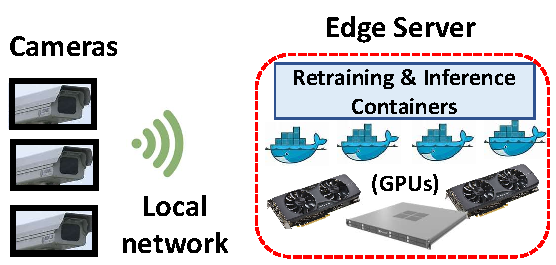
\includegraphics[width=0.6\columnwidth]{ekya/figures/xxx_cropped.pdf}
     \caption{Cameras connect to the edge server, with consumer-grade GPUs for DNN inference and retraining containers.%. We propose extending the workload to include continuous retraining of DNNs.
     }
     \label{fig:edge}
 \end{figure}

Thus, due to reasons of network cost and video privacy, it is preferred to run both inference and retraining on the edge compute device itself without relying on the cloud. In fact, with bandwidths typical in edge deployments, cloud-based solutions are slower and result in lower accuracies (\S\ref{subsec:eval-alternate}).

\subsection{Compressed DNN models and data drift}
\label{subsec:continuous}

Advances in computer vision research have led to high-accuracy DNN models that %surpass human-level accuracy on general images and videos. These DNN models 
achieve high accuracy with a large number of weights, deep architectures, and copious training data. While highly accurate, using these heavy and general DNNs for video analytics is both expensive and slow \cite{noscope, DBLP:conf/osdi/HsiehABVBPGM18}, which make them unfit for resource-constrained edge computing. The most common approach to addressing the resource constraints on the edge is to train and deploy \emph{specialized and compressed} DNNs \cite{compression-4, compression-5, compression-6, compression-17, compression-18, compression-19}, which consist of far fewer weights and shallower architectures. \revtext{For instance, Microsoft's edge video analytics platform ~\cite{rocket-blog} uses a compressed DNN (TinyYOLO~\cite{redmon2018yolov3}) for efficiency. Similarly, Google released Learn2Compress\cite{learn2compress} for edge devices to automate the generation of compressed models from proprietary models.} These compressed DNNs are trained to only recognize the limited objects and scenes specific to each video stream. In other words, to maintain high accuracy, they forego generality for improved compute efficiency \cite{noscope, DBLP:conf/osdi/HsiehABVBPGM18, mullapudi2019}. 

% use cases - connected smart cars, indexing on iphone, even stationary traffic cameras
%Advances in DNN efficiency, e.g., using model compression \cite{compression-4, compression-5, compression-6, compression-17, compression-18, compression-19}, have enabled the deployment of DNN models on resource-constrained edge servers. Efficient edge models drive video analytics applications in modern cars, urban mobility traffic control, and enterprise campuses \cite{bellevue-report}. %Video analytics in smart cars already provide safety assist features (e.g., lane drift alerts) and many more such features are expected in the near future \cite{smart-cars}. Camera streams in enterprise buildings are analyzed for security applications as well as for ubiquitous sensing applications, e.g., face recognition to authenticate building access \cite{smart-buildings}. %Mobile devices use DNN object classifiers to generate ``tags'' for the pictures and videos clicked by users, thus enabling search by keywords (e.g., find pictures with a party hat) \cite{iphone-indexing}. 
%\junchen{this para could be a good fit to a new subsection of ``DNN deployed at the edge''?}
%\junchen{i like the idea of starting with data drift, though maybe we should motivate why data drift is so damaging in the first place? }

%\begin{figure}[t!]
%  \centering
%  \begin{subfigure}[t]{0.5\linewidth}
%    \centering
%    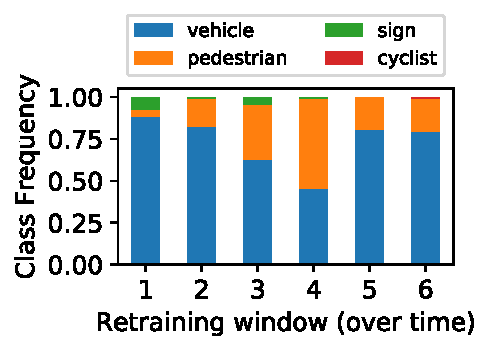
\includegraphics[width=\linewidth]{ekya/ekya/figures/motivation/incr_learn_motivation/motivation_waymo_distchange_classdist.pdf} 
%    \caption{Class distribution}
%    \label{fig:class-distrib-motivation}
%  \end{subfigure}
%  ~~~
%  \begin{subfigure}[t]{0.5\linewidth}
%    \centering
%    % \includegraphics[width=\linewidth]{ekya/figures/motivation/Class_Incrementality/class_distribution_change_sf_27.png}
%    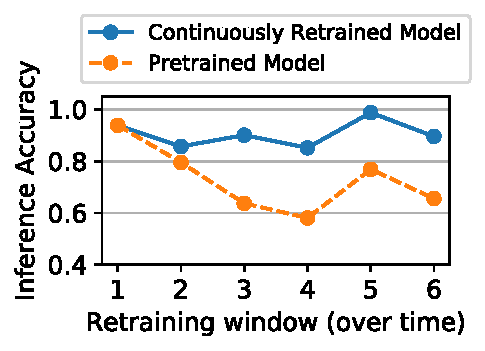
\includegraphics[width=\linewidth]{ekya/figures/motivation/incr_learn_motivation/motivation_waymo_distchange_acc.pdf}
%     \caption{Accuracy}
%    \label{fig:class-distrib-motivation-acc}
%  \end{subfigure}
%  \caption{Impact of changing class distribution (left) on model accuracy in the Waymo data. Continuous learning results in higher and steady accuracy over time (right). \kh{Update the figures to include the one trained with first half of the tasks}}
%  \label{fig:waymo-motivation-distrib}
%\end{figure}


\noindent{\bf Data drift.} As specialized edge DNNs have shallower architectures than general DNNs, they can only memorize limited amount of object appearances, object classes, and scenes. As a result, specialized edge DNNs are particularly vulnerable to {\em data drift} \cite{datadrift-7, datadrift-8, datadrift-a, datadrift-b}, where live video data diverges significantly from the initial training data. For example, variations in the object pose, scene density (e.g. rush hours), and lighting (e.g., sunny vs. rainy days) over time make it difficult for traffic cameras to accurately identify the objects of interest (cars, bicycles, road signs). Cameras in modern cars observe vastly varying scenes (e.g., building types, crowd sizes) as they move through different neighborhoods and cities. Further, the {\em distribution} of the objects change over time, which reduces the edge model's accuracy \cite{distribution-20, distribution-21}. Due to their ability to memorize limited amount of object variations, edge DNNs have to be continuously updated with recent data and changing object distributions to maintain a high accuracy.  %Finally, newer object classes may appear (e.g., segway scooters) which may not have been available in the initial training data \cite{incremental-24, icarl-14}.  

%\vspace{-.05in}\subsubsection{\bf Data drift.} %While model compression has considerably increased the inference efficiency of DNN models, it also results in their having lower ``capacity'' to learn from their training data. 
%While compressed models are initially trained on representative data, when they are out in the field, they suffer from {\em data drift} \cite{datadrift-7, datadrift-8, datadrift-a, datadrift-b}. Data drift refers to the live video data diverging significantly from the initial training data. For example, traffic cameras encounter many variations in the angles of objects, scene density, and lighting over time, thus making it difficult to accurately identify the objects of interest (cars, bicycles, road signs).  
%Cameras in modern cars observe vastly varying scenes (e.g., building colors, crowd sizes) as they move through different neighborhoods and cities. %\ion{Are we considering cameras in slefdriving cars? If yes, I'm not sure about it. First, cars can have very powerful processors. Second, I don't think that we can easily sell the point about degrading inference to do the training in such a mission critical app (just add a second processor for inference). Third, not sure we want to deploy a model in a self-driving car without careful validation.} 


%The problem of data drift is exacerbated in compressed models. Compression of DNNs makes them efficient in their compute and memory demands, and facilitates their deployment on resource-constrained edge servers. However, smaller DNNs can memorize less due to their relatively limited capacity. In other words, their efficiency comes at the expense of generalizability to the data distributions of live inference videos that are different than their training data \cite{compressiondrift-22, compressiondrift-23, efficientnet-3}. %It is generally difficult to provide an exhaustive training dataset with enough samples to cover all possible variations.
%It is difficult and often intractable to provide an exhaustive training dataset with enough samples to cover all possible variations, especially in open real-world deployments. 

%\ga{Model capacity drops due to compression?} \junchen{to Ganesh's comment on compression vs. capacity: totally agree this is what any (knowledgeable) reviewer may wonder as well. i believe there {\em is} a fundamental tradeoff between capacity (how much to compress) and generalizability (robustness to data drift).maybe just cite the ECCV paper Romil found and ask Nikolas for more.} \ys{+1 on this point. The large the model is, the higher capacity it has. However, a large model not only requires a huge amount of data and time for training, but also leads to a higher runtime cost (memory, latency etc.) during inference. Hence, an alternative of having a large well-trained model is to maintain a localized cheaper model, and retrain it on demand. }

\noindent{\bf Continuous training.} The preferred approach, that has gained significant attention, is for edge DNNs to {\em continuously learn} as they incrementally observe new samples over time \cite{incremental-13, icarl-14, incremental-15}. %while not fully forgetting the learnings from old samples. 
The high temporal locality of videos allows the edge DNNs to focus their learning on the most recent object appearances and object classes \cite{DBLP:conf/cvpr/ShenHPK17, mullapudi2019}.  
%Incremental learning techniques %retain snapshots of history for the retraining (not the entire historical dataset) and  avoid {\em catastrophic forgetting} of the learnings on historical data \cite{datadrift-8} even as they learn from new data. 
%In \name, we use a modified version of iCaRL \cite{icarl-14} though our techniques are generally applicable.
In \name, we use a modified version of iCaRL\cite{icarl-14} learning algorithm to on-board new classes, as well as adapt to the changing characteristics of the existing classes. %We also tune the balance distillation and cross-entropy losses. 
%We use the iCaRL \cite{icarl-14} incremental learning algorithm for our experiments though the techniques in our work are generally applicable.
%In our solution, 
Since manual labeling is not feasible for continuous training systems on the edge, \revtext{the labels for the retraining are obtained from a ``golden model'' - a highly accurate (87\% and 84\% accuracy on Cityscapes and Waymo datasets, respectively) but expensive model (deeper architecture with large number of weights)}. The golden model cannot keep up with inference on the live videos and we use it to label only a small fraction of the videos in the retraining window. %\revtext{We then use these labels from the golden model to train compressed models.} 
Our approach is essentially that of supervising a low-cost ``student'' model with a high-cost ``teacher'' model (or knowledge distillation \cite{44873}), and this has been broadly applied in computer vision literature \cite{incremental-13, mullapudi2019, incremental-15, distribution-20}. %The use of a golden model for labeling is consistent with prior work in computer vision literature \cite{incremental-13, mullapudi2019, incremental-15, distribution-20}. 


% data drift; class incremental; waymo graphs; app-level impact
\subsection{Accuracy benefits of continuous learning}
\label{subsec:continuous-measurement}

\begin{figure}[t!]
  \centering
  % Accuracy figure
  % Class distribution figure
  \begin{subfigure}[t]{0.42\linewidth}
    \centering
    % 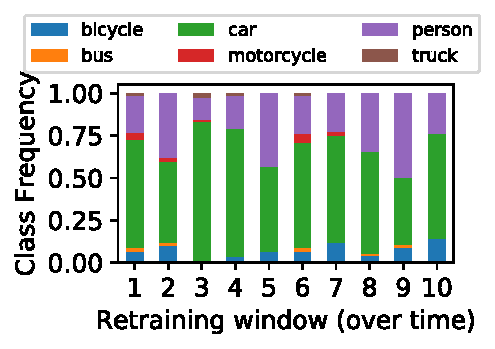
\includegraphics[width=\linewidth]{ekya/figures/motivation/incr_learn_motivation/motivation_jena_classdist.pdf}
    % 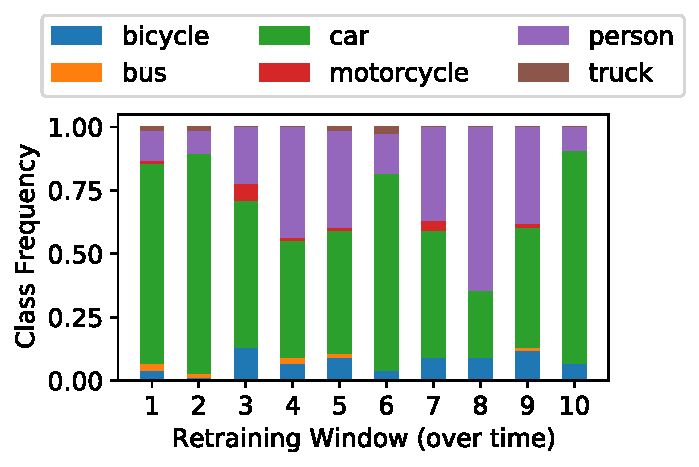
\includegraphics[width=\linewidth]{ekya/figures/motivation/incr_learn_motivation/motivation_cityscapes_jena_classdist.pdf}
    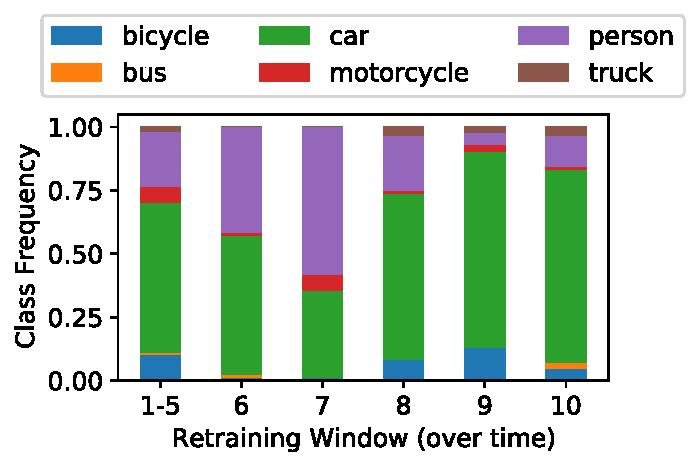
\includegraphics[width=\linewidth]{ekya/figures/motivation/incr_learn_motivation/motivation_cityscapes_zurich_classdist.pdf}
    \caption{Class Distribution}
    \label{fig:jena-classdist}
  \end{subfigure}
    ~~
  \begin{subfigure}[t]{0.42\linewidth}
    \centering
    % 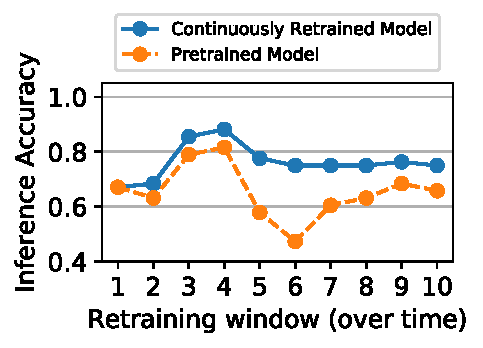
\includegraphics[width=\linewidth]{ekya/figures/motivation/incr_learn_motivation/motivation_jena_acc.pdf}
    % 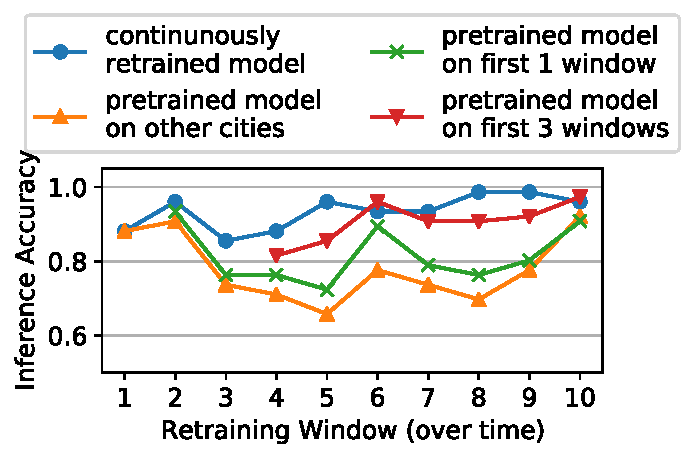
\includegraphics[width=\linewidth]{ekya/figures/motivation/incr_learn_motivation/motivation_cityscapes_jena_accuracy.pdf}
    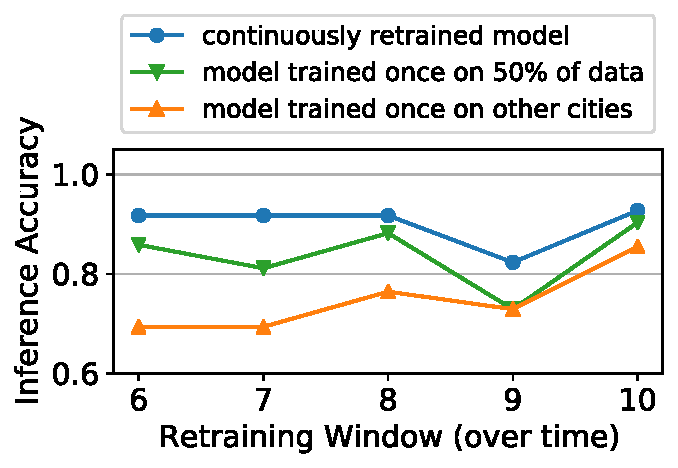
\includegraphics[width=\linewidth]{ekya/figures/motivation/incr_learn_motivation/new_motivation_cityscapes_zurich_accuracy.pdf}
    
    
    \caption{Accuracy}
    \label{fig:jena-motivation}
  \end{subfigure}
    \hspace*{\fill}
  ~~
  % Sample Image Task 1
  \begin{subfigure}[t]{0.41\linewidth}
    \centering
    % 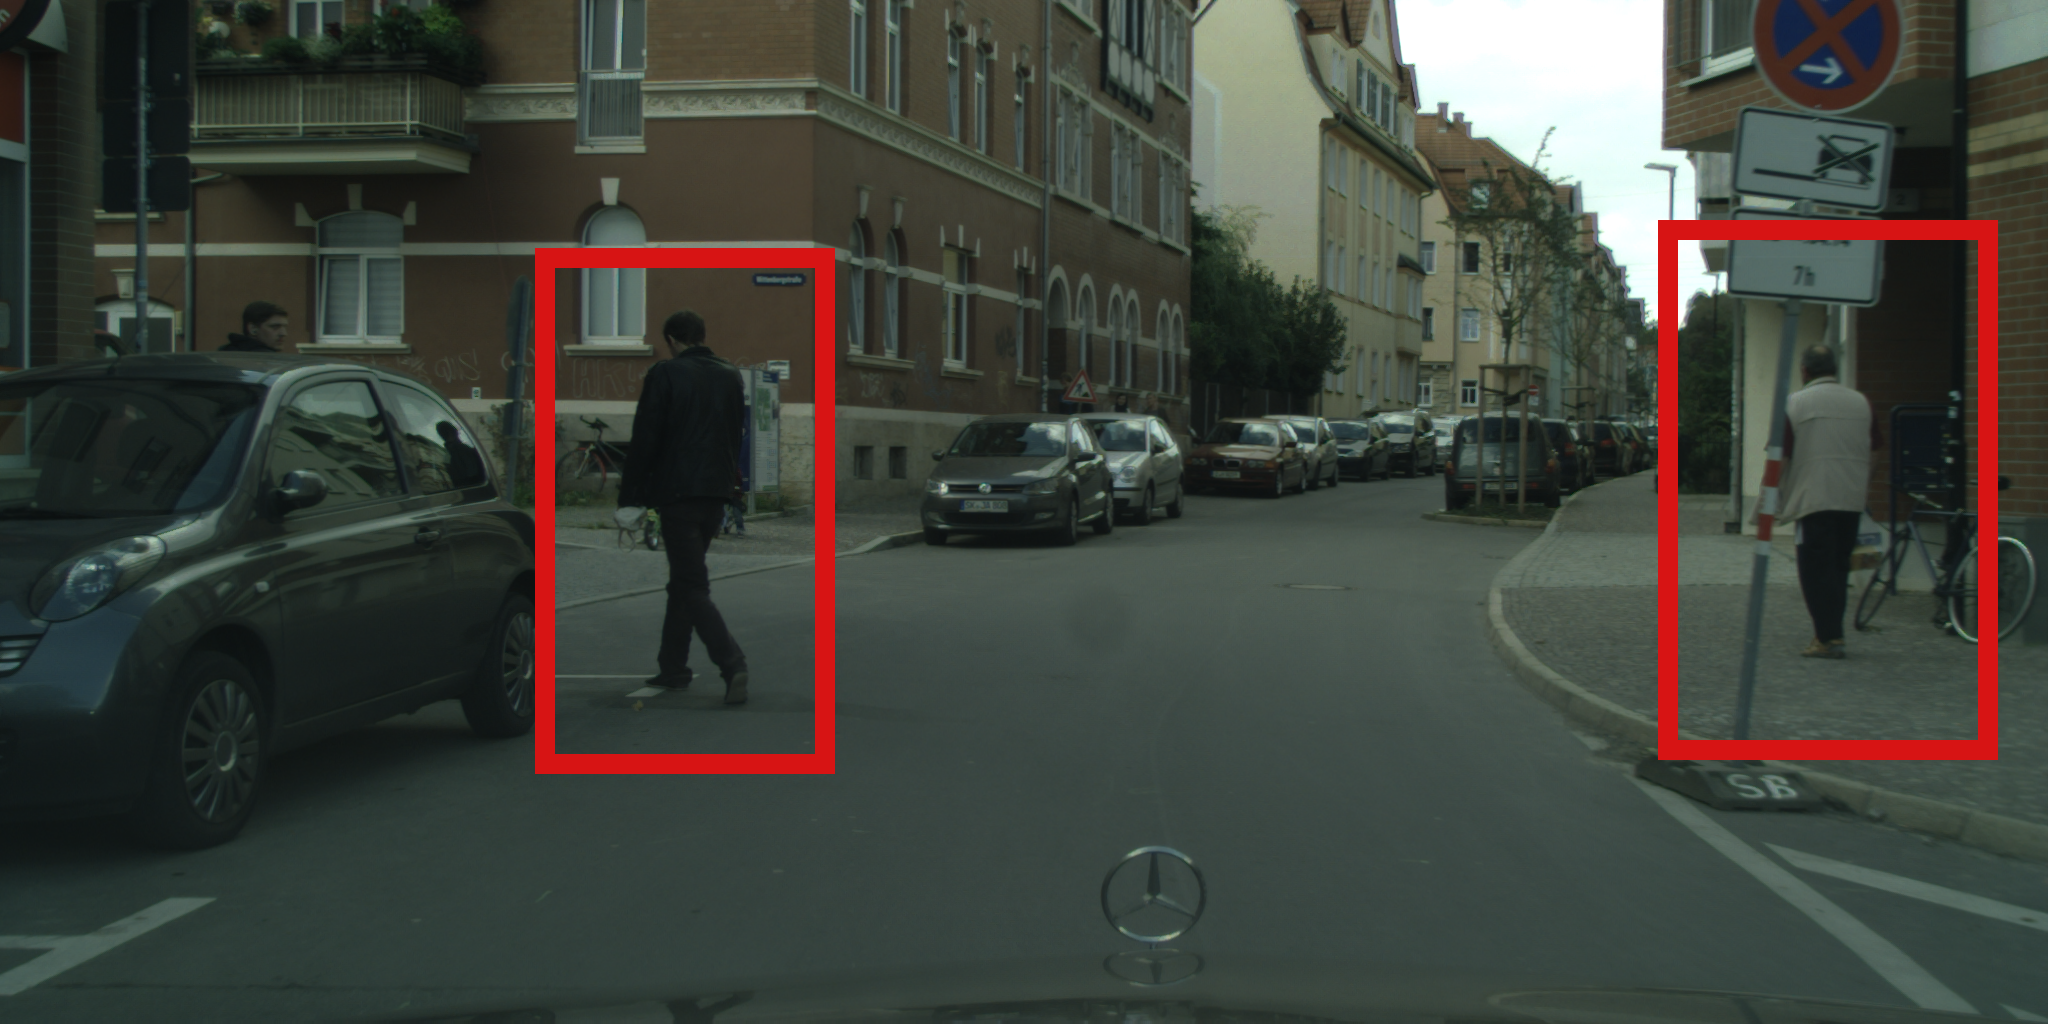
\includegraphics[width=\linewidth]{ekya/figures/motivation/incr_learn_motivation/t1_marked.png}
    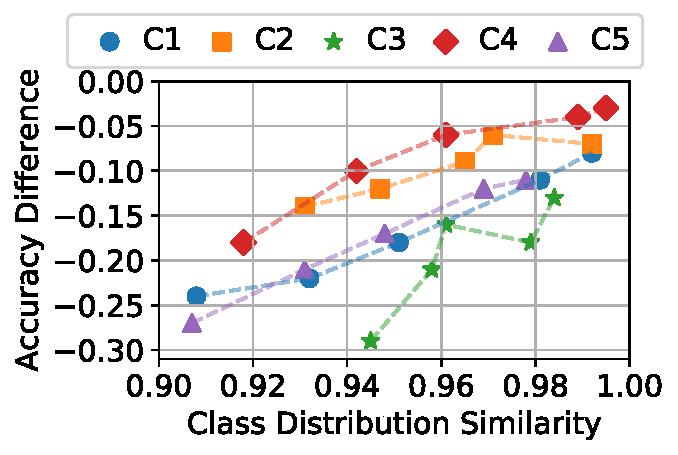
\includegraphics[width=\linewidth]{ekya/figures/motivation/incr_learn_motivation/motivation_datadrift_vs_acc.pdf}
     \caption{Accuracy vs data drift}
    \label{fig:acc-datadrift}
  \end{subfigure}
  ~~
  % Sample Image Task 6
  \begin{subfigure}[t]{0.41\linewidth}
    \centering
    % 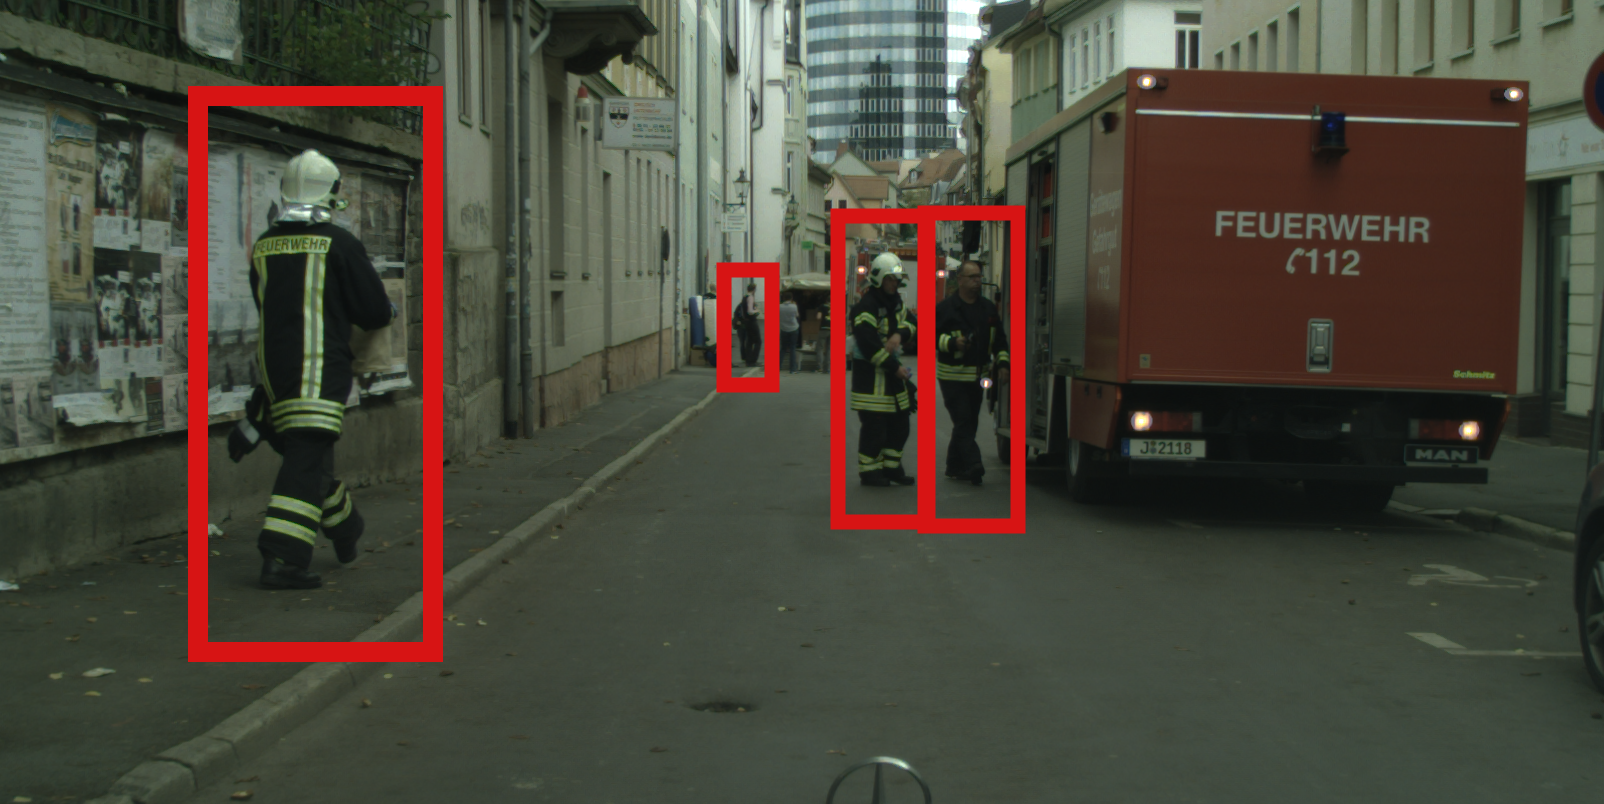
\includegraphics[width=\linewidth]{ekya/figures/motivation/incr_learn_motivation/t6_marked.png}
    % 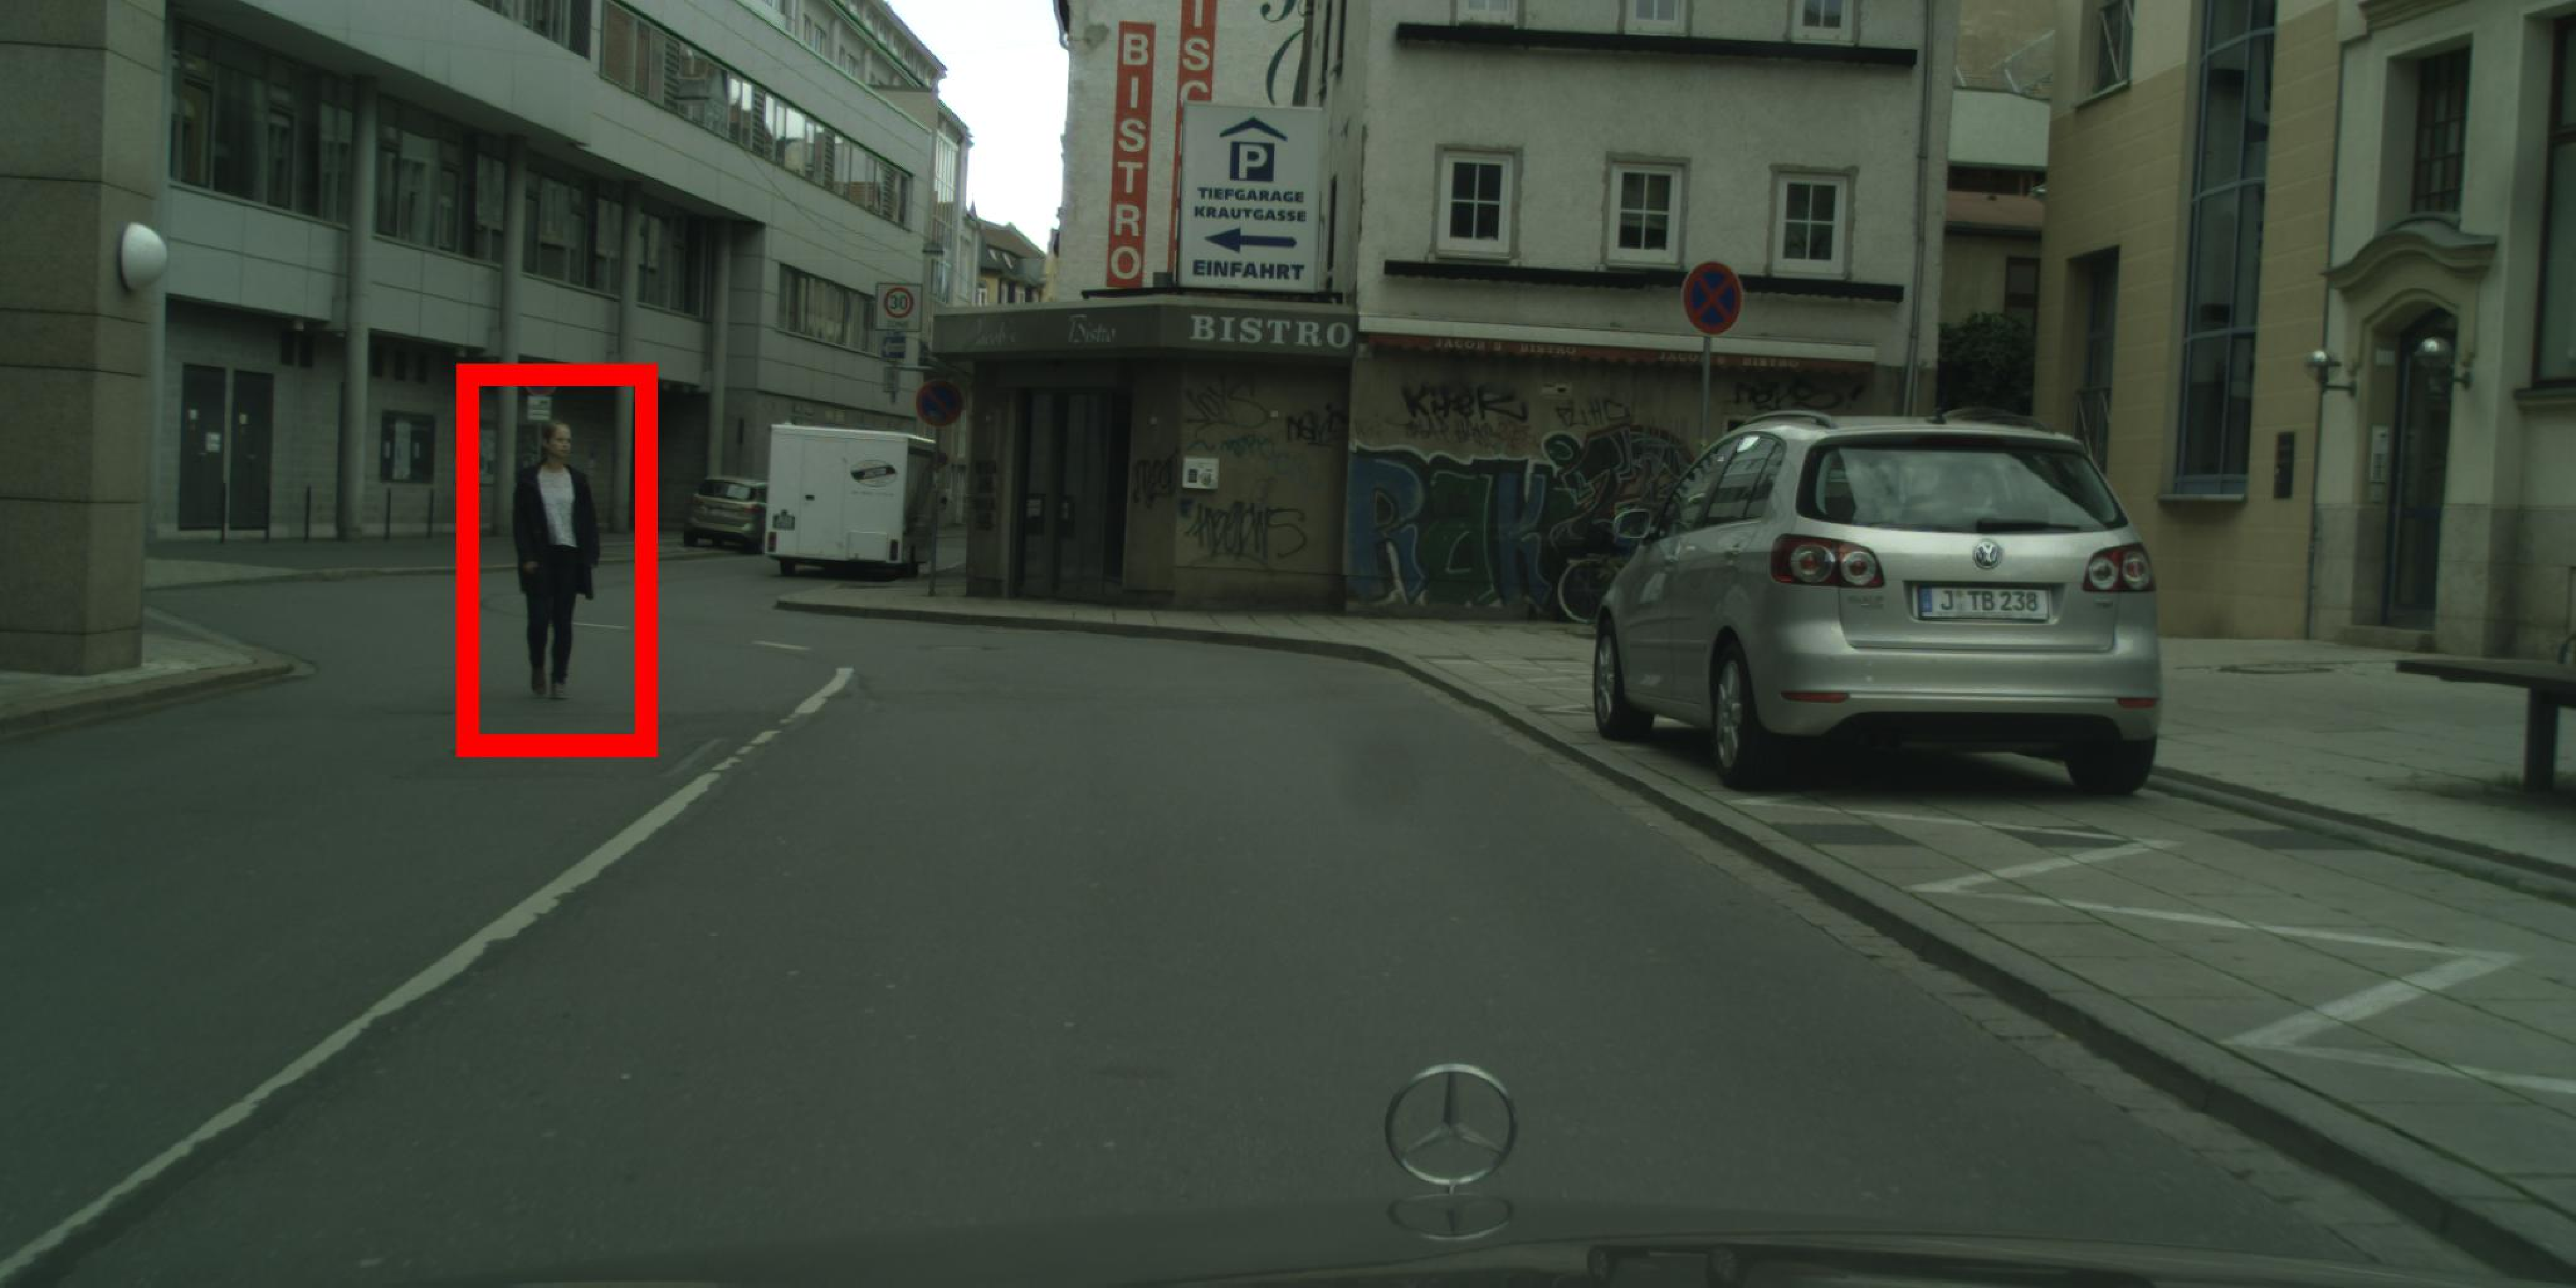
\includegraphics[width=\linewidth]{ekya/figures/motivation/incr_learn_motivation/motivation_cityscapes_jena_win5.pdf}
    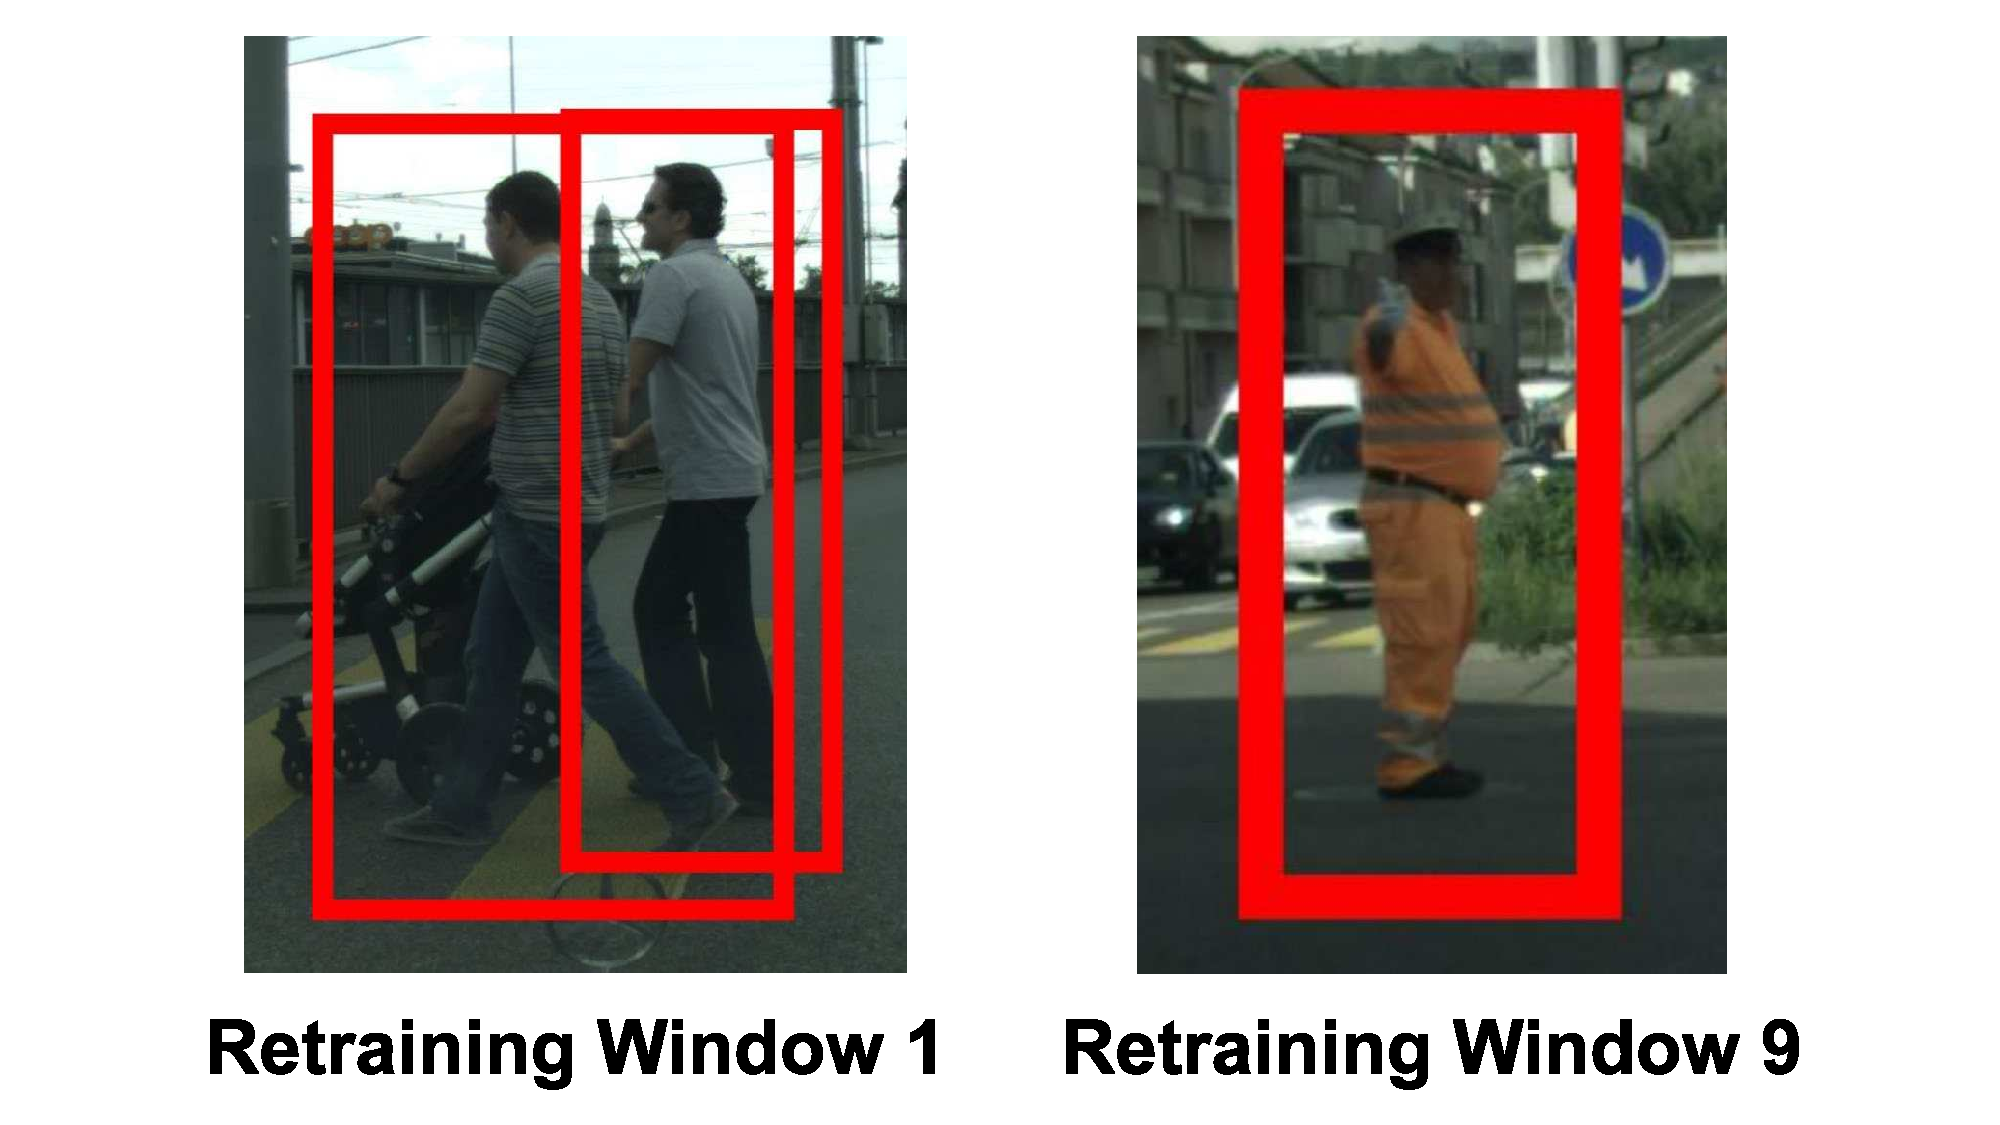
\includegraphics[width=\linewidth]{ekya/figures/motivation/incr_learn_motivation/person_classshift.pdf}
    \caption{Person class variations}
    \label{fig:personclass}
  \end{subfigure}
  
   \caption{\cameratext{Continuous learning in the Cityscapes dataset. Shift in class distributions (a) across windows necessitates continuous learning (b). Model accuracy is not only affected by class distribution shifts (c), but also by changes in object appearances (d).}}% As more data samples are made available to model for retraining, it achieves a higher accuracy compared to a pre-trained model which does not adapt to the new data samples. We evaluate the accuracy of the following classes -- 'person', 'car, 'truck', 'bus', 'bicycle', 'motorcycle'.}
  \label{fig:cityscapes-motivation}
\end{figure}



%To show the benefits of continuous learning, we use two video datasets that were collected from dashboard cameras in cars: Cityscapes \cite{cityscapes} in Europe and Waymo \cite{waymo} in the USA. These cameras collect data samples over time and at different locations. (Details of the datasets in \S\ref{subsec:eval-setup}). 

To show the benefits of continuous learning, we use the video stream from one example city in the Cityscapes dataset \cite{cityscapes} that consists of videos from dashboard cameras in many cities. %over time and at different locations. 
In our evaluation in \S\ref{sec:evaluation}, we use both moving dashboard cameras as well as static cameras over long time periods. 
We divide the video data in our example city into ten fixed \emph{retraining windows} (200s in this example). 


\noindent\cameratext{\textbf{Understanding sources of data drift.} Figure \ref{fig:jena-classdist} shows the change of object class distributions across windows. The initial five windows see a fair amount of persons and bicycles, but bicycles rarely show up in windows 6 and 7, while the share of persons varies considerably across windows $6-10$. Figure~\ref{fig:acc-datadrift} summarizes the effect of this data drift on model accuracy in five independent video streams, C1-C5. For each stream, we train a baseline model on the first five windows, and test it against five windows in the future and use cosine similarity to measure the class distribution shift for each window. Though accuracy generally improves when the model is used on windows with similar class distributions (high cosine similarity), the relationship is not guaranteed (C2, C3). This is because class distribution shift is not the only form of data drift. Illumination, pose and appearance differences also affect model performance (e.g. clothing and angles for objects in the person class vary significantly; Figure \ref{fig:personclass}).}

\noindent\cameratext{\textbf{Improving accuracy with continuous learning.}} Figure \ref{fig:jena-motivation} plots inference accuracy of an edge DNN (a compressed ResNet18 classifier) in the last five windows using different training options. 
%: (1) pretrain the model with representative data from \kh{10} other cities in the same dataset; (2) pretrain the model with recent history (the first five windows) in the same video; and (3) continuously retrain the model in every window. 
%$(1)$ Starting with an off-the-shelf ResNet18 model that was trained on the ImageNet dataset \cite{DBLP:journals/ijcv/RussakovskyDSKS15} and further tuned 
$(1)$ Training a compressed ResNet18 with video data on all other cities of the Cityscapes dataset does not result in good performance.
%Note that tuning off-the-shelf models using related datasets is common in deployments. 
$(2)$ Unsurprisingly, we observe that training the edge DNN once using data from the first five windows {\em of this example city} improves the accuracy. %by $9\%$ on average. 
$(3)$ %However,  
%We observe that the pretrained model using all data from \kh{4} other cities performs poorly. Similarly, using data from the first five windows to pretrain the edge DNN also suffers from accuracy drops in the next five windows. Both results show the limitation of pretraining edge DNNs with large and representative data.  
%In contrast, 
{\em Continuous retraining} using the most recent data for training achieves the highest accuracy consistently. Its accuracy is higher than the other options %first two offline training options 
by up to $22\%$.%$ $15\%$ and $6\%$, respectively.  %and its accuracy is much higher and more consistent. 
%Its accuracy is up to \kh{$25\%$} higher than the pretrained DNNs in one window. On average across all windows, continuous retraining leads to \kh{$10\%$ to $20\%$} higher accuracy over the pretrained DNNs. 

\revtext{Interestingly, using the data from the first five windows to train the larger ResNet101 DNN (not graphed) achieves better accuracy than the continuously retrained ResNet18.}  %While this gap indicates the %presence of data drift and the 
%benefit of using the most recent data for training, 
The substantially better accuracy of ResNet101 compared to ResNet18 when trained {\em on the same data} of the first five windows also shows that this training data was indeed fairly representative. But the lightweight ResNet18's weights and architecture limits its ability to learn and is a key contributor to its lower accuracy.
%This shows that the data in the first five windows is in fact fairly representative, but the ResNet18 model's cheaper weights and architecture is a key factor contributing to its lower accuracy. 
Nonetheless, ResNet101 %is unsuited for live video inference as it takes $50-260$ms per inference on edge class GPUs \cite{cnn-perf}, which 
is $13\times$ slower than the compressed ResNet18 \cite{cnn-perf}. % which makes the latter more suited for edge deployments.
%cost of $50-260$ms per inference on edge class GPUs 
%. 
This makes the efficient ResNet18 more suited for edge deployments and continuous learning enables it to maintain high accuracy even with data drift. Therefore, the need for continuous training of edge DNNs is ongoing and not just during a ``ramp-up'' phase. %We use the even more expensive \gaa{ResNext101} as our golden model for labeling, and we have verified that its results almost match manual labeling.
% Efficiency between ResNet101 and ResNet18 Ref: https://github.com/jcjohnson/cnn-benchmarks
% Our measured 
% is unable to memorize all the data.



%even though the edge DNN is pretrained with \kh{10$\times$} of data samples from the same dataset.  
%As Figure \ref{fig:jena-classdist} shows, class distribution changes quickly over time. The initial training samples are dominated by vehicles, but a lot more pedestrians and motorcycles show up at later time. 
%The appearance of objects also changes significantly, such as pedestrians show up in different clothing and angles at different time (Figure \ref{fig:jena-image-1} and \ref{fig:jena-image-6}).
%Figure \ref{fig:jena-motivation} shows that such data shift causes major accuracy drop for edge DNNs (ResNet18 in this example) that are pretrained with data from other cities. 
%We also see considerable accuracy drop even when the edge DNN is retrained with the same video in the first one and first three windows.


%Retraining window $6$ in Figure \ref{fig:cityscapes-motivation} highlights an interesting aspect. The distributions of classes in window \kh{$6$} and window \kh{$1$} are similar (Figure \ref{fig:jena-classdist}), yet the continuously retrained model achieves much higher accuracy than the model that is pretrained with data in window \kh{$1$} (Figure \ref{fig:jena-motivation}). Visual inspection suggests that this difference is likely due to the varying appearance and angles of objects (e.g., people with different clothing) between the two windows; see Figures \ref{fig:jena-image-1} and \ref{fig:jena-image-6}.% Thus, continuous learning is valuable even when the class

%Figure \ref{fig:waymo-motivation-distrib} illustrates how class distribution and DNN inference accuracy change over time in one city in the Waymo dataset, and the results are shown in fixed \emph{retraining windows} (\kh{xx} seconds in this example). 
%As Figure \ref{fig:class-distrib-motivation} shows, class distribution changes significantly over time. The initial training samples are dominated by vehicles, but a lot more pedestrians and road signs show up at later time. 
%As Figure \ref{fig:class-distrib-motivation-acc} shows, this data shift causes major accuracy drop for edge DNNs (ResNet18 in this example) that are pretrained with offline data in the same dataset. 
%We also see considerable accuracy drop even when the edge DNN is retrained with the \emph{first half} of the video in this camera.
%In contrast, the continuously retrained DNN keeps using recent data to cope with the changing distributions, and it achieves \kh{$xx\%$ and $yy\%$} higher accuracy over the DNNs that are pretrained with the offline and first half video data, respectively. We observe similar phenomenon in all other cities in the Waymo dataset, as continuously retrained edge DNNs achieve \kh{xx\%} higher accuracy over pretrained edge DNNs on average (up to \kh{yy\%}). \footnote{In Figures \ref{fig:waymo-motivation-distrib} and \ref{fig:cityscapes-motivation}, at each retraining window $i$ on the x-axis, the data from ($i-2, i-1$) is used for retraining the model, and the data from ($i-1, i$) is used for inference (testing), whose accuracy in turn is plotted on the y-axis.}

%Figure \ref{fig:class-distrib-motivation} demonstrates the impact of changes to the distribution of object classes in (a single city of the Waymo data) on the ResNet18 classifier. We compare the accuracies of a continuously updated ResNet18 classifier against the version of ResNet18 that was pre-trained only once initially (on a few samples from this video). 
%Further, continuous learning is also beneficial when the {\em distribution} of data samples of the object classes changes over time; Figure \ref{fig:class-distrib-motivation}. 
%While the initial training samples are dominated by vehicles, more examples of pedestrians  and road signs become available with time (Figure \ref{fig:class-distrib-motivation}). This is typical of video data in suburban cities where the pedestrian traffic is considerably lower than vehicular traffic. The changing distribution causes the once-trained ResNet18's accuracy to drop while the continuously trained model keeps retraining itself with the recent data, copes with the changing distributions, and achieves $28\%$ higher accuracy (Figure \ref{fig:class-distrib-motivation-acc}). \footnote{In Figures \ref{fig:waymo-motivation-distrib} and \ref{fig:cityscapes-motivation}, at each retraining window $i$ on the x-axis, the data from ($i-2, i-1$) is used for retraining the model, and the data from ($i-1, i$) is used for inference (testing), whose accuracy in turn is plotted on the y-axis.}




% sample incremental; jena and tubingen of cityscapes
%Figure \ref{fig:cityscapes-motivation} shows the benefits of {\em sample-incremental} training, i.e., improving the model with newer data samples over time. %We use two videos for this experiments from cars driving in two cities, Jena and Tubingen. 
%We compare the accuracies of the continuously updated ResNet18 convolutional classifier against the version of ResNet18 that was trained only once initially (on a few representative samples before the edge model was deployed). 

%Figure \ref{fig:cityscapes-motivation} shows the similar phenomenon of the impact of changing class distributions (Figure \ref{fig:jena-classdist}) with the Cityscapes data (again, a single city). 
%As Figure \ref{fig:jena-motivation} shows, continuously retrained DNN achieves much higher (by \kh{$zz\%$}) and more steady accuracy than the pretrained DNNs.
%Across all cities in the Cityscapes dataset, continuously retrained DNNs achieve \kh{xx\%} higher accuracy over pretrained edge DNNs on average (up to \kh{yy\%} higher).
%while the accuracies of the two models -- continuously-trained and once-trained -- are similar at the beginning, over time, continuous learning leads to the model's accuracy being higher (by $27\%$) and relatively steady. % they diverge over time to a difference of as much as $27\%$ in accuracy. Continuous learning results in relatively steady (and higher) accuracy over time. %We observe a similar trend in Figure \ref{fig:tubingen-motivation} where the divergence in accuracy due to not updating the model is observed immediately. (Note that in each of Figure \ref{fig:jena-motivation} and \ref{fig:tubingen-motivation} our experiments use new data samples over time obtained from a {\em single} city.)  
%Retraining window $6$ in Figure \ref{fig:cityscapes-motivation} highlights an interesting aspect. The distributions of classes in window \kh{$6$} and window \kh{$1$} are similar (Figure \ref{fig:jena-classdist}), yet the continuously retrained model achieves much higher accuracy than the model that is pretrained with data in window \kh{$1$} (Figure \ref{fig:jena-motivation}). Visual inspection suggests that this difference is likely due to the varying appearance and angles of objects (e.g., people with different clothing) between the two windows; see Figures \ref{fig:jena-image-1} and \ref{fig:jena-image-6}.% Thus, continuous learning is valuable even when the class distributions are similar.

%%Comparing against a version of the model that is trained on representative data initially is conservative because typical deployments use off-the-shelf models that are pre-trained on standard datasets (e.g., ImageNet \cite{imagenet} or MS-COCO \cite{coco}). 
%%%%%Our experiments, overall, demonstrate the value of improving the models with new data samples to cope with changing data distributions as well as changing conditions and appearances of the objects. 
%\junchen{hmm.. i do see the point that having more samples helps, but in any event, people will use a model (even a cheap one) trained offline with some {\em large} standard dataset (imagenet, coco, etc). i tend to believe the gain is due to fine-tuning the ResNet model to in-situ data from the Cityscape ``scene'' and more such data the better?}
%%Continuous learning also helps to learn altogether new object classes, whose examples may not have been included in the training data \cite{incremental-24, icarl-14}.
%\noindent{\bf Rate of change.} Finally, different videos change at different rates. Urban settings typically observe higher change in their data distributions and will benefit from more frequent retraining, while suburban settings will do with a relatively lower retraining frequency. Likewise, times of busy traffic see a faster change in their data distributions compared to off-peak periods. In addition, the data distributions are also significantly different {\em across cities} (even if they are neighboring) in both the Waymo and Cityscapes datasets. Models that are deployed in vehicles moving across neighboring cities at different times will benefit from learning on new data. 

%We observe similar phenomenon across a diverse set of videos (see \S\ref{sec:evaluation}). Edge DNNs that are pretrained only once experience significant accuracy drop over time, even if their training data is from the same video in the recent history. These sharp accuracy drops make the inference results inconsistent and unreliable.  In contrast, continuous training enables edge DNNs to adapt with the most recent and relevant data, and it leads to much higher and more steady accuracy. 



%\begin{figure}[t!]
%  \centering
%  \begin{subfigure}[t]{0.5\linewidth}
%    \centering
%    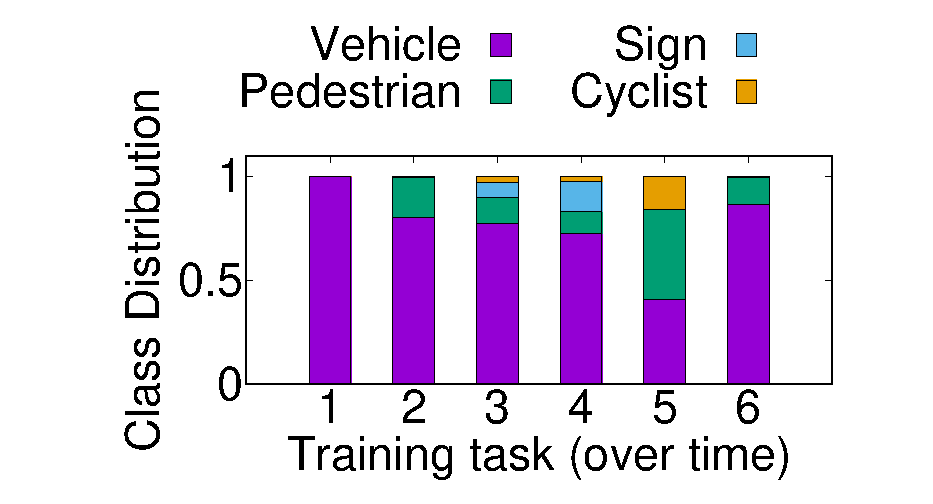
\includegraphics[width=\linewidth]{ekya/figures/motivation/Class_Incrementality/new_class.eps}
%    \caption{New classes over time}
%        \label{fig:class-inc-motivation}
%  \end{subfigure}
%  ~~
%  \begin{subfigure}[t]{0.5\linewidth}
%    \centering
%    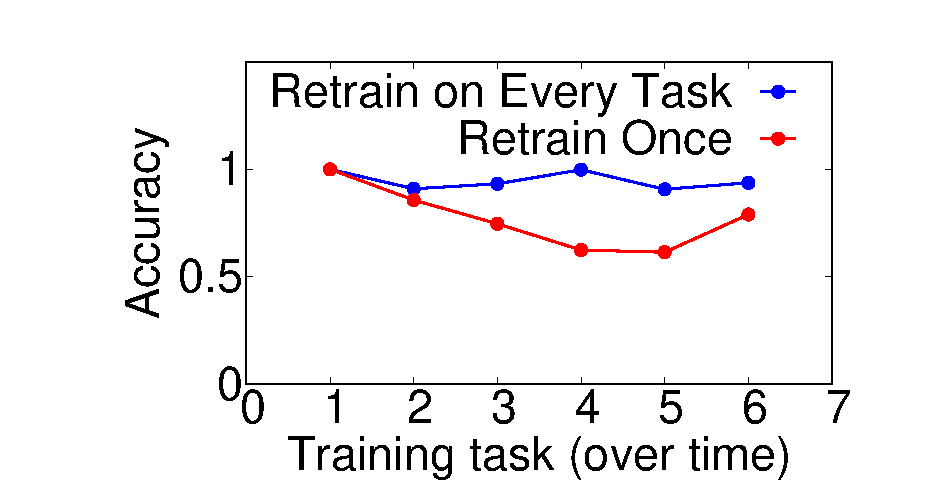
\includegraphics[width=\linewidth]{ekya/figures/motivation/Class_Incrementality/new_class_acc.eps}
%    \caption{Accuracy}
%        \label{fig:class-inc-motivation-acc}
%  \end{subfigure}
%   \hfill
%  ~~
%  \caption{Class incremental learning with Waymo.}
%  \label{fig:waymo-motivation}
%\end{figure}

%{\em Class-incremental} training refers to learning new object classes with time, thus expanding the model's classification targets. As shown in Figure \ref{fig:class-inc-motivation}, the initial training data only consists of samples of vehicles, but over time, pedestrians, road signs, and cyclists are added. Continuously updating the ResNet18 model to include these new classes results in consistently higher accuracy by as much as $37\%$ (Figure \ref{fig:class-inc-motivation-acc}). \ion{This example is a bit contrived. Why would you even consider deploying a model for video traffic that is trained only on cars in the first place?}


% impact of different retraining frequencies - show variation across two cities
%\ga{TODO paragraph.} \textbf{Retraining Frequency.} As a model specializes for a specific data distribution, its performance on general data decreases.  Moreover, frequent retraining requires more resources, which may not be available and thus the model may be trained only for a shorter duration \romil{The inference-resource-opportunity-cost argument can also be put here, but is not reflected in the plots}. Thus, a high retraining frequency can reduce the model accuracy.
%\junchen{Is retraining too frequently lowers the accuracy because of more frames being dropped or because of retraining ending prematurely for lack of resource? if so, please make it explicit. i was confused as reader..}
%This is observed in \cref{fig:cologne-motivation} and \cref{fig:erfurt-motivation}, where having just 2 tasks \romil{Explain what a task is} has a mean accuracy of 70.4\% over the entire dataset, but decreases to 69.8\% when retrained over 10 tasks. Similar behavior for Erfurt (82.9\% vs 82.2\%). 


% golden model; can retain more info but is expensive; edge model's capacity is less but is cheaper to execute
% show graph - golden, edge w/ retraining, edge w/o retraining (for one of the above cities); both sample and class incremental
% romilb: a third line in figure 1 - (showing continuously high accuracy?) 

%\noindent{\bf Golden model.}



% used for inference already; we propose running training too; storage isn't a concern but compute is limited; the network is also a worry, so we cannot access the infinite compute in the cloud
%\subsection{\bf Joint inference and retraining on edge servers.}
%Our proposal is to extend the edge servers, which already performs video DNN inferences, to {\em include continuous training of the edge DNN models}. Edge servers already have capacity to store the limited amount of recent video data that is required for continuous retraining. However, its compute capacity is a concern as the edge server's compute is already provisioned for the DNN inference on live video streams. Since retraining is periodic, i.e., its compute requirements are bursty in nature, provisioning compute resources for retraining will lead to wasted utilization and increased cost (by as much as \gaa{XXX} in our experiments). For the reasons explained in \S\ref{subsec:edge} regarding bandwidth constraints and privacy sensitivities, transmitting the videos to the cloud for retraining is not preferred. 
%As we describe next, we develop techniques to minimize disruption to the inference while smartly allocating resources for continuous retraining. %maximize the eventual inference accuracy. 


\section{Motivation}
\label{sec:motivation}

% Gandiva. Problems - conflicting policies, elastic scaling to more nodes, dynamic scheduling policy when jobs change, composable policies
%\name{} is motivated by the challenges faced by applications in exercising fine-grained control over scheduling of compute resources  in a distributed environment. Consider Gandiva\cite{gandiva}, a system for distributed training of machine learning jobs which builds on Kubernetes \cite{kubernetes} for task orchestration. Gandiva applies compute and data co-locality and load-balancing through mechanisms such as time-sharing and task migration to speed up hyperparameter search in machine learning experiments. Co-locality avoids network overheads between jobs running across GPUs, while load-balancing ensures the workload is evenly split across the cluster to avoid network and compute bottlenecks. Additionally, some model-parallel jobs may require all-or-none scheduling semantics \cite{shivaram-gpustudy}, where all task instances requested by the job must run concurrently for it to progress.

\name{} is motivated by the need of many modern applications to have fine-grained scheduling control in a distributed environment. Consider Gandiva\cite{gandiva}, a system for distributed training of neural networks that builds on top of Kubernetes\cite{kubernetes}. Gandiva has a diverse set of scheduling requirements, including co-locality, load-balancing, and gang scheduling. In particular, Gandiva uses co-location of data and computation to avoid unnecessary data transfers, load-balancing to split the work evenly across the cluster to avoid stragglers, and gang-scheduling to ensure that the training job makes progress. 

Gandiva's scheduling requirements exposes two challenges. First, some of these requirements are conflicting. On one hand, Gondiva wants to  co-locate some tasks on the same node; on the other hand, it wants to evenly distribute (i.e., load-balancing) tasks across the cluster. Second, Gandiva's scheduling policy can be naturally expressed as an hierarchical composition of simple policies: gang schedule some sets of tasks, where these sets are load balanced across the cluster, and where tasks in the same set are co-located on the same machine. Unfortunately, expressing this composition is challenging both for the application and the underlying execution framework: the framework must be general enough to support arbitrary scheduling policies, and the application must be able to express these requirements, as well as resolve the conflicts between these requirements. %todo: Highlight that only applications know how to resolve conflicts.

%These scheduling requirements have two notable characteristics, which can be observed generally across modern distributed applications. First, the application has seemingly divergent scheduling requirements - for instance, some sets of Gandiva tasks need to be co-located on the same node, while others need to be evenly spread across the cluster. Second, the overall scheduling policy of the application can be expressed as a hierarchical composition of simpler policies. In Gandiva, the scheduling policy is a composition of task co-location, followed by load-balancing and finally gang-scheduling applied to tasks belonging to the same job. These scheduling requirements present challenges for both, the application and the underlying execution framework - applications must be able to express their specific scheduling requirements, while frameworks must be general enough to support arbitrary scheduling policies. %todo: Highlight that only applications know how to resolve conflicts.
 
% Explore existing solution space
% 1) Write custom scheduler
For frameworks which offer only a fixed set of scheduling policies to choose from, the approach to expressing custom policies is to modify the core scheduler in the framework. However, this is undesirable for multiple reasons. First, modifying existing scheduler code can be arduous and requires a deep understanding of the working of the framework. Second, any changes in the core of the framework may introduce bugs. Finally, it creates a strong dependence between the application and the framework, limiting the portability to other frameworks.

% 2) Expose Mechanisms to Control
% 2a) Direct scheduler API
Many frameworks recognize the need to extend scheduling control to applications and offer mechanisms to support heterogenous application-level scheduling objectives. Some frameworks \cite{kubernetes} expose control in the form of REST APIs, where applications can query the list of waiting tasks and specify the precise node where the task must be scheduled. While this offers fine grained control over scheduling and portability, this approach has several drawbacks. First, this introduces a single point for failure for the entire scheduling subsystem. Frameworks may want to employ distributed schedulers for performance and robustness, but this approach reverts them to a centralized scheduler residing in the application. Second, it promotes a tight coupling between tasks and physical nodes. This is undesirable when nodes can fail or are transient in nature, like in a serverless computing environment, making fault-recovery difficult. Third, the application is burdened with implementing a scheduler whereas it only requires the ability to specify policies at a high level.

% 2b) Resource management API
Some frameworks \cite{yarn, mesos} assume that applications' scheduling objectives are strongly tied with allocation of physical resources. Following this motivation, these frameworks provide scheduling control through the proxy of resource management. For instance, \cite{mesos} extends opportunistic resource offers and applications may choose to accept and utilize these resources as they require. This mechanism simplifies the application layer logic since the complexity of implementing a full-fledged scheduler is abstracted away, but it limits the flexibility of applications to express compositions of policies which may extend beyond physical resources. For instance, a combination of load-balancing and co-location is challenging with this mechanism since the tasks are bound to each other rather than physical resources.  

% Highlight common problems, and how ExoSched solves them.
Thus, the challenge is to provide clean and flexible interfaces for applications to express heterogenous scheduling requirements without leaking the complexity of scheduling mechanisms. \name{} is a scalable new scheduler design that rethinks resource management to expose high level scheduling policy control. By having the ability to create custom resource labels at runtime, applications can express their scheduling requirements in \name{}, while the core scheduler remains lean and minimalist.  
%\textcolor{red}{TODO: Improve the last paragraph.}

% Simple examples
%todo(romilb): Should this be a general application
% Consider a Reinforcement Learning application that must train an agent on a GPU and then evaluate this agent in a CPU intensive environment simulation. To scale beyond a single machine, this application can leverage a distributed execution framework to launch multiple instances of these agents and environments across the compute resources available to it. However, the placement of these instances is critical to the application's performance - the agent and it's associated environment must be scheduled on the same physical node to avoid network overheads while evaluating the agent. Thus, the challenge is to convey this scheduling requirement to the execution framework.


%!TEX root = main.tex
%!TEX spellcheck = en_US 



\section{{Ekya}: Solution Description}
\label{sec:solution}







% Src: https://docs.google.com/drawings/d/1nBnwhi1agkQVHhFf01fLEV5nnQofWXlroUTv8ZCXxuw/edit?usp=sharing

% We start by formally defining our resource allocation problem (\S\ref{subsec:formulation}). In \S\ref{subsec:thief} and \S\ref{subsec:misc} we explain the design of our scheduling solution {\name} and its different features.

% We first formally define our joint retraining and inference with limited resource problem (\S\ref{subsec:formulation}). 
% We then explain the scheduling algorithm of \name (\S\ref{subsec:thief}) and how it estimates performance gains of various schedules (\S\ref{subsec:profiling}), before highlighting optimizations to address practical issues such as performance estimation errors (\S\ref{subsec:misc}).

%\subsection{Overview}
%\label{subsec:overview}


% overview
Continuous training on limited edge resources requires smartly deciding when to retrain each video stream's model, how much resources to allocate, and what configurations to use. Making these decisions presents two challenges.

First, the decision space of multi-dimensional configurations and resource allocations is computationally more complex than two fundamentally challenging problems of multi-dimensional knapsack and multi-armed bandits (\S\ref{subsec:formulation}). %, thus it is very expensive to explore the space of decisions. 
Hence, we design a {\bf thief scheduler} (\S\ref{subsec:thief}), 
% At the core of {\name} is its resource manager, that we refer to as 
a heuristic that makes the joint retraining-inference scheduling tractable in practice. % by exploring a relatively small yet beneficial fraction of the space of decisions. 
%We first formalize the joint retraining-inference scheduling under limited resource and analyze its complexity (\S\ref{subsec:formulation}). The thief scheduler makes the problem tractable in practice, by exploring a relatively small yet promising fraction of action space.
%, thus significantly reducing the problem complexity.

Second, the scheduler requires the model's exact performance (in resource usage and inference accuracy), but this requires retraining using all the configurations. 
%it is infeasible to know a model's exact performance (in resource usage and inference accuracy) for all retraining configurations, as it requires actual retraining and labeling using all configurations. However, this information is essential for the decision making.
We address this challenge with our {\bf micro-profiler} (\S\ref{subsec:profiling}), which retrains only a few select configurations on 
%which profiles the accuracies of many of retraining configurations by actually using them to retrain the model, but 
a fraction of the data. Figure \ref{fig:sys-arch} presents an overview of {\name}'s components. % with early termination.%, and does so only for a small number of promising configurations.  %and for a small number of training epochs, and then gradually prune the set of promising configurations. 

%To maximize the benefit of retraining, {\name}'s decision making and performance estimation must be fast and resource-efficient. 
%Our techniques (in \S\ref{subsec:thief} and \S\ref{subsec:profiling}) address both challenges. % drastically reduce the cost of decision making and performance estimation. %by at least two orders of magnitude when compared to \gaa{traditional solutions} while reaping the accuracy benefits from retraining. 
% to manage the inference and retraining of multiple videos at an edge server. 
% misc
%As shown, \name also includes practical solutions to a range of challenges in a continuous retraining system (\S\ref{subsec:misc}).



%We build upon the thief scheduler to support checkpointing of models {\em during} retraining (\S\ref{subsubsec:checkpoint}) to provide the inference with more accurate models sooner. 
%{\name} also {\em dynamically reallocates resources} when it detects errors in the resource-accuracy estimations (\S\ref{subsubsec:error-profiles}). %We describe the other factors that impact continuous training in \S\ref{subsec:misc}. 
%Generating the resource-accuracy estimations of the retraining jobs is described in \S\ref{sec:profiling}.


%\begin{table}[t!]
\small
\begin{tabular}{cl}
{\bf Notation} & {\bf Description}\\\hline
$V$ & Set of video cameras\\
$v$ & Single video camera\\\hline
$G$ & Total GPU resources\\
$g^v_R$ & Resources for retraining video stream $v$\\
$g^v_I$ & Resource for inference on video stream $v$\\\hline
$\Gamma_v$ & Set of all configurations for retraining $v$\\
 & (each configuration is referred to as $\gamma_v$)\\
$\Lambda_v$ & Set of all configurations for inference on $v$\\
 & (each configuration is referred to as $\lambda_v$)\\\hline
$a_v$ & Accuracy of inference on video stream $v$\\
$\alpha_v$ & Accuracy of inference over time window\\
$T$ & Retraining window duration\\\hline\\
\end{tabular}
\caption{\label{tab:notations}\small\bf Notations used in {\name}'s description.}
\end{table}

\subsection{\hspace{-0.2cm}Formulation of joint inference-retraining scheduling}
\label{subsec:formulation}
% Setup
We maximize the inference accuracy of all video streams in a retraining window. Table \ref{tab:notations} has the list of relevant notations.
We consider a pool of edge GPUs $G$ (each edge server might have a few GPUs~\cite{azure-ase}) shared by the inference and retraining jobs of a set of video streams $V$, with video $v$($\in V$)'s inference job getting $g^{v}_I$ GPU resources and its training job getting $g^{v}_R$ GPU resources\footnote{\junchen{need to clarify why we only share GPU cycles, not RAM, etc.}}. 
For each video $v \in V$, we denote its inference accuracy $a_v$, which could be improved by retraining.
$\gamma_v$ is the retraining configuration, picked from a pool of \textit{configurations} $\Gamma_v$, to retrain the model of video $v$.
$\lambda_v$ is the inference configuration (e.g., frame sampling rate), picked from an inference resource-accuracy profile $\Lambda_v$ \cite{videostorm, chameleon}, to run the inference job of video $v$.
Note that inference configurations are always chosen such that its resource demand does not exceed the allocation $g^v_I$ for inference.

Given the retraining and inference configurations ($\gamma_v,\lambda_v$) and resource allocations ($g^{v}_R, g^{v}_I$) of a video $v$, its inference accuracy at time $t$ is
$a_v(t, g^v_R, \gamma_v, g^v_I, \lambda_v)$ and inference accuracy measured over the retraining window $T$ can be expressed by 
\[
\alpha_v (T) = \frac{1}{T} \int_{t=0}^{T} a_v(t, g^v_R, \gamma_v, g^v_I, \lambda_v)\ dt
\]


%Edge deployments have one or few edge servers that have multiple video cameras $V$ streaming to them for analytics (\S\ref{subsec:edge}). The analytics on the video streams in $V$ share the same GPU resource pool $G$ (typically, a few GPUs per edge server \cite{azure-ase}). For each video stream $v \in V$, there is a continuous inference job whose inference accuracy is $a_v$. A retraining job is run periodically per video stream which improves $a_v$. The resource pool $G$ must be split across the inference and retraining jobs of all video streams, with video $v$'s inference job getting $g^{v}_I$ GPU resources and its training job getting $g^{v}_R$ GPU resources. Table \ref{tab:notations} has the list of relevant notations.



% Training Profiles. Not going into details on how performance scales with resources..
%Every retraining job of video $v$ has a pool of \textit{configurations} $\Gamma_v$ (\S\ref{subsec:profiles}). Each configuration $\gamma_v \in \Gamma_v$ specifies the hyperparameters and an associated accuracy-resource\_time profile. Increased resource allocation to training grants more resource\_time to the training job, allowing it to achieve a higher accuracy for the same wall\_time. Once a retraining job completes, it updates the inference job with the new model. Similar to the training configurations, the inference job of each camera $c$ has a inference performance profile, which dictates the scaling of the inference accuracy as the inference resource allocation changes.
%\noindent{\bf Configurations:} Every retraining job of video $v$ has a pool of \textit{configurations} $\Gamma_v$. Each configuration $\gamma_v \in \Gamma_v$ specifies the hyperparameters and its accuracy (see \S\ref{subsec:profiles}). Increasing resource allocation to retraining ($g^v_R$) allows it complete faster and update the inference job sooner with the new model.% with higher accuracy. 
%
%The inference job of each video stream $v$ also has a resource-accuracy profile $\Lambda_v$ \cite{videostorm, chameleon}, with each configuration $\lambda_v \in \Lambda_v$ (e.g., frame sampling rate) in the profile specifying the current inference accuracy ($a_v$) as well as the resource {\em demand} to keep up with the processing of the live video stream. %All the inference configurations can keep up with processing the live video stream if its corresponding resource demand is allocated, but their accuracies will vary. % which dictates the scaling of the inference accuracy as the inference resource allocation changes.
%Inference configurations are always chosen such that its resource demand does not exceed the allocation $g^v_I$ for inference.

% Define inference accuracy.
%\noindent{\bf Inference accuracy over time:} 
%The inference accuracy of a video $v$ measured over the retraining window depends on the inference configuration (which in turn depends on its resources allocation $g^v_I$) as well as the inference model (pre-retraining and post-retraining). The accuracy of the model post-retraining depends on the retraining configuration $\gamma_v \in \Gamma_v$ and the GPU allocation to the retraining $g^v_R$. Thus, for a video stream $v$ whose inference accuracy at any point in time is $a_v$, the inference accuracy $\alpha_v$ averaged over time $t=0 \rightarrow T$ is (where $T$ is the retraining window):
%\[
%\alpha_v (T) = \frac{1}{T} \int_{t=0}^{T} a_v(t, g^v_R, \gamma_v, g^v_I, \lambda_v)\ dt
%\]

% Objective - What are the metrics and why
\noindent The joint retraining-inference optimization maximizes the average accuracy over a retraining window across all videos through selecting configurations ($\gamma_v$ and $\lambda_v$) and allocating resource between retraining ($g^{R}_v$) and inference ($g^{I}_v$):
\begin{equation}
    \begin{aligned}
        & \underset{g_{R}^v, g_{I}^v, \gamma_v, \lambda_v}{\text{maximize}}
        %& & \frac{\sum_{v \in V}\alpha_v(T, g_{R}^v, \gamma_v, g_{I}^v, \lambda_v)}{|V|} \\
        & & \frac{\sum_{v \in V}\alpha_v(T)}{|V|} \\
        & \text{s.t.}
        & & \sum_{v \in V} g_{R}^v + g_{I}^v \leq G\\
        %&&& a_v(t, g_{R}^v, \gamma_v, g_{I}^v, \lambda_v) \geq a_\text{MIN} \\
        &&& a_v(t) \geq a_\text{MIN}, \forall v \in V, 0 \leq t \leq T 
        %TODO(romilb): Cleanup this min accuracy expression
    \end{aligned}
    \label{eqn:optimization}
\end{equation}
The joint retraining-inference scheduling essentially balances the inference accuracy before retraining finishes and the optimization of long-term accuracy by finishing model retraining as soon as possible.
This fundamentally differs from optimization for only inference accuracy or only training accuracy in two aspects.
Additionally, we allow for the inference accuracy $a_v$ at any point in time to be bounded by a minimum $a_\text{MIN}$ (application-specific bound), so that the inference results remain useful to the application, especially when the model is being retrained.


%As shown in \S\ref{subsec:motivation-sched-example}, optimizing for only the inference accuracy or only the retraining accuracy does not maximize the inference accuracy over the retraining window, $\alpha_v (T)$. % over all cameras $v \in V$. 
%%optimizing for maximum training accuracy is immaterial since the goal is not just to retrain the model, but also use it while it is still useful. Thus the objective is to maximize the mean inference accuracy across all cameras $C$ present in the system by picking the correct configurations and resource allocations, constrained by the size of the resource pool available.
%% https://jcnts.wordpress.com/2009/11/11/formatting-optimization-problems-with-latex/
%%\noindent{\bf Optimization formulation:} 
%
%We seek to maximize the average inference accuracy over the retraining window $T$ (i.e., $\alpha_v(T)$) across all videos $v \in V$ by picking the configurations $\gamma_v$ and $\lambda_v$ for each video stream $v$'s retraining and inference, and allocating the edge's GPU resource $G$ for retraining ($g^{R}_v$) and inference ($g^{I}_v$). Additionally, we allow for the inference accuracy $a_v$ at any point in time to be bounded by a minimum $a_\text{MIN}$ (application-specific bound), so that the inference results remain useful to the application.

% computationally intractable
\mypara{Complexity analysis}
The complexity of the above optimization is combinatorial in the number of configurations and cameras. As a result, we proceed to devise an efficient scheduling heuristic.% that provides good results in practice.
\junchen{Kevin, the complexity discussion can be here}






\subsection{Formulation of joint inference and retraining}
\label{subsec:formulation}

The problem of joint inference and retraining aims to maximize overall inference accuracy for all video streams $\mathcal{V}$ in a retraining window ${T}$ with duration $\lVert T \rVert$. 
All work must be done in $\mathcal{G}$ GPUs.
Thus, the total compute capability is $\mathcal{G}\lVert T \rVert$ GPU-time. Without loss of generality, let $\delta$ be the smallest granularity of GPU allocation.  %(e.g., if $\delta = 1\%$ of GPU, $150\delta =$ 1.5 GPU). Let $\Theta$ be the set of all possible GPU allocations $\Theta = \{0, 1, ..., \frac{\mathcal{G}}{\delta}\}$.
Each video $v \in V$ has a set of \emph{retraining} configurations $\Gamma$
and a set of \emph{inference} configurations $\Lambda$ (\S\ref{subsec:profiles}).
Table \ref{tab:notations} (\S{\ref{appendix:scheduler}}) lists the notations. 



\noindent\textbf{Decisions.} For each video $v\in\mathcal{V}$ in a window $T$, we decide: (1) the retraining configuration $\gamma\in\Gamma$ ($\gamma = \emptyset$ means no retraining); (2) the inference configuration $\lambda\in\Lambda$; and (3) how many GPUs (in multiples of $\delta$) % (in terms of GPU resource units $\delta$)
to allocate for retraining ($\mathcal{R}$) %\in\Theta$) 
and inference ($\mathcal{I}$). %\in\Theta$). 
We use binary variables $\phi_{v\gamma\lambda\mathcal{R}\mathcal{I}}\in\{0,1\}$ to denote these decisions (see Table \ref{tab:notations} \S{\ref{appendix:scheduler}} for the definition). 
These decisions require $C_T(v, \gamma, \lambda)$ GPU-time and yields overall accuracy of $A_T(v, \gamma, \lambda, \mathcal{R}, \mathcal{I})$. $A_T(v, \gamma, \lambda, \mathcal{R}, \mathcal{I})$ is averaged across the window $T$ (\S\ref{subsec:motivation-sched-example}), and the above decisions determine the inference accuracy at {\em each point in time}.
%Specifically, let $a_t(v, \gamma, \lambda, \mathcal{R}, \mathcal{I})$ be the inference accuracy for video $v$ at a point in time $t$, % given retraining configuration $\gamma$, inference configuration $\lambda$, $\mathcal{R}\delta$ GPUs for retraining, and $\mathcal{I}\delta$ GPUs for inference, we have:
%\[
%\ A_T(v, \gamma, \lambda, \mathcal{R}, \mathcal{I}) = 
%\frac{1}{\lVert T \rVert} \int_{t=0}^{\lVert T \rVert} a_t(v, \gamma, \lambda, \mathcal{R}, \mathcal{I})\ dt
%\]


%At each retraining window $t \in \mathcal{T}$, the system maintains a set of DNN instances $M_{v}^t$ for video $v$, where each $m_{v\gamma}^t \in M_{v}^t$ denotes a DNN instance that is trained based on configuration $\gamma$. Each DNN $m_{v\gamma}^0 \in M_{v}^0$ is pretrained with offline video data. 
%The system can optionally retrain $m_{v\gamma}^t$ into $\hat{m}_{v\gamma}^t$ with training configuration $\gamma$ and the video data of $v$ at $t$, and the retraining cost is $C^R(v, t, \gamma)$.

%The system must pick a DNN $m_{v\gamma}^t$ or $\hat{m}_{v\gamma}^t$ and an inference configuration $\lambda \in \Lambda$ to run inference for video $v$ at $t$.
%The inference cost of such a decision is $C^I(v, t, \gamma, \lambda$), and the inference accuracy is $A(v, t, m, \lambda)$ where $m$ is the chosen DNN. 
%We use binary variables $r_{vt\gamma g}$ and $i_{vt\gamma \lambda g}$ to indicate the decisions made by the system (see Table \ref{tab:notations} for their definitions).

\noindent\textbf{Optimization.} Maximize the inference accuracy averaged across all videos in a retraining window within the GPU limit. 

{\small
\vspace{-12pt}
\begin{equation}
    \begin{aligned}
    %\footnotesize
       & \underset{\phi_{v\gamma\lambda\mathcal{R}\mathcal{I}}}{\arg\max}
         \frac{1}{\lVert \mathcal{V} \rVert}
         \sum_{\substack{\forall v\in\mathcal{V}, 
                        \forall \gamma\in\Gamma,
                        \forall \lambda\in\Lambda,\\
                        \forall \mathcal{R}, \forall \mathcal{I} \in \{0, 1, ..., \frac{\mathcal{G}}{\delta}\} %\in \Theta,
                        %\forall \mathcal{I} \in \Theta
                        }}
          \phi_{v\gamma\lambda\mathcal{R}\mathcal{I}} \cdot
          A_T(v, \gamma, \lambda, \mathcal{R}, \mathcal{I})\\
       & \text{subject to}\\
       & 1. \sum_{\substack{\forall v\in\mathcal{V}, 
                        \forall \gamma\in\Gamma,
                        \forall \lambda\in\Lambda,\\
                        \forall \mathcal{R}, \forall \mathcal{I}}}
                        \phi_{v\gamma\lambda\mathcal{R}\mathcal{I}} \cdot
                        C_T(v, \gamma, \lambda)
                        \leq \mathcal{G}\lVert T \rVert \\
      & 2. \sum_{\substack{\forall v\in\mathcal{V},
                        \forall \gamma\in\Gamma,
                        \forall \lambda\in\Lambda,\\
                        \forall \mathcal{R}, \forall \mathcal{I}}}
                           \phi_{v\gamma\lambda\mathcal{R}\mathcal{I}} \cdot
                           (\mathcal{R} + \mathcal{I})
                        \leq \frac{\mathcal{G}}{\delta} \\
      & 3. \sum_{\substack{\forall \gamma\in\Gamma, 
                           \forall \lambda\in\Lambda,\\ 
                           \forall \mathcal{R}, %\in \Theta,
                           \forall \mathcal{I}}} %\in \Theta}}
           \phi_{v\gamma\lambda\mathcal{R}\mathcal{I}} \leq 1, 
           \forall v\in\mathcal{V}
    \end{aligned}
    \label{eqn:optimization}
\end{equation}
}%

The first constraint ensures that the GPU allocation does not exceed the available GPU-time $\mathcal{G}\lVert T \rVert$ in the retraining window. The second constraint limits the {\em instantaneous}  allocation (in multiples of $\delta$) to never exceed the available GPUs. 
%The third constraint ensures that the system can only pick at most one retraining configuration/allocation and one inference configuration/allocation for each video $v$.
The third constraint ensures that at most one configuration is picked for retraining and inference each for a video $v$.





% https://docs.google.com/drawings/d/1nBnwhi1agkQVHhFf01fLEV5nnQofWXlroUTv8ZCXxuw/edit?usp=sharing
%\begin{figure*}[t!]
%    \centering
%    \includegraphics[width=0.85\linewidth]{ekya/figures/Solution/"Ekya System Architecture Arch".pdf}
%    \caption{{\name} System Architecture. \ga{Make it a one-column figure.}}
%    \label{fig:sys-arch}
%\end{figure*}

% % rest of the section
% \subsection{Solution Overview}
% \label{subsec:overview}

% Figure \ref{fig:sys-arch} presents an overview of {\name} to manage the inference and retraining of videos at an edge server. At the core of {\name} is its resource manager, that we refer to as ``thief'' scheduler, which is a greedy scheduling heuristic (\S\ref{subsec:thief}). We build upon the thief scheduler to support checkpointing of models {\em during} retraining (\S\ref{subsubsec:checkpoint}) to provide the inference with more accurate models sooner. {\name} also {\em dynamically reallocates resources} when it detects errors in the resource-accuracy estimations (\S\ref{subsubsec:error-profiles}). %We describe the other factors that impact continuous training in \S\ref{subsec:misc}. 
% Generating the resource-accuracy estimations of the retraining jobs is described in \S\ref{sec:profiling}.
%\revtext{This optimization problem can be expressed as a multi-dimensional binary knapsack problem while the uncertainty of $A_T(v, \gamma, \lambda, \mathcal{R}, \mathcal{I})$ can be modelled as multi-armed bandits (MAB) problem. A detailed complexity analysis is presented in \S\ref{complexity-analysis}.}
Our analysis in \S\ref{complexity-analysis} shows that the above optimization problem is {\em harder} than the multi-dimensional binary knapsack problem and modeling the uncertainty of $A_T(v, \gamma, \lambda, \mathcal{R}, \mathcal{I})$ is more challenging than the multi-armed bandit problem.
%\ga{Summarize the complexity analysis.}


\begin{figure}[ht]
    \centering
    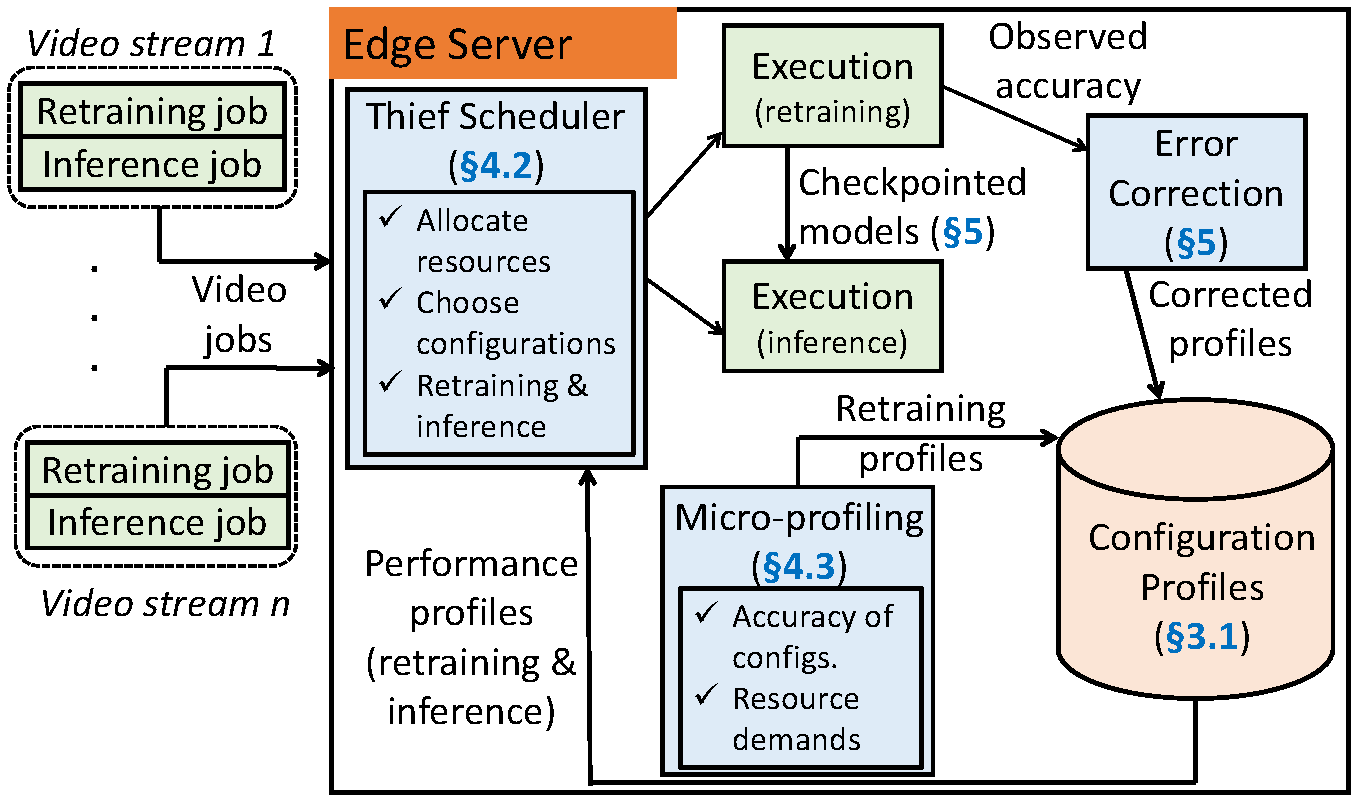
\includegraphics[width=.85\columnwidth]{ekya/figures/overview_cropped.pdf}
    \caption{{\name}'s components and their interactions. }%\ga{Update with the right section numbers.}}
    \label{fig:sys-arch}
\end{figure}

\subsection{Thief Scheduler}
\label{subsec:thief}




%The computational intractability of the formulation in \S\ref{subsec:formulation} stems primarily from jointly allocating resources and picking configurations. In this section, we decouple the two and develop an efficient and iterative heuristic (Algorithm \ref{algo:thief_sched}). 
Our scheduling heuristic makes the scheduling problem tractable by decoupling resource allocation (i.e., $\mathcal{R}$ and $\mathcal{I}$) and configuration selection (i.e., $\gamma$ and $\lambda$) (Algorithm \ref{algo:thief_sched}). %It iteratively allocates resources to all inference and retraining jobs and picks inference/retraining configurations within the limit of the allocated resource. 
%We present the heuristic and then explain the key assumptions and relaxations that it is built upon. 
%\textbf{Challenge:} Equation \ref{eqn:optimization} requires that both the resource allocation and the configurations must be picked jointly. One influences the other, thus we present an iterative algorithm \ref{algo:thief_sched} which tries to converge on the optimal (?) combination.
We refer to {\name}'s scheduler as the ``thief'' scheduler and it iterates among all inference and retraining jobs as follows.% and picks inference/retraining configurations within the limit of the allocated resource. %configuration selection as follows. 
%\begin{packeditemize}

%\item 
{\bf (1)} It starts with a fair allocation for all video streams $v \in V$ (line 2 in Algorithm \ref{algo:thief_sched}). 
In each step, it iterates over all the inference and retraining jobs of each video stream (lines 5-6), and {\em steals} a tiny quantum $\Delta$ of resources (in multiples of $\delta$; see Table \ref{tab:notations}, \S\ref{appendix:scheduler}) from each of the other jobs (lines 10-11).

%\item 
{\bf (2)} With the new resource allocations ({\small temp\_alloc[]}), it then selects configurations for the jobs using the {\sf\footnotesize PickConfigs} method (line 14 and Algorithm \ref{algo:pickconfigs}, \S{\ref{appendix:scheduler}}) that iterates over all the configurations for inference and retraining for each video stream.  
For inference jobs, among all the configurations whose accuracy is $\geq a_\text{MIN}$, {\sf\footnotesize PickConfigs} picks the configuration with the highest accuracy that can keep up with the inference of the live video stream given current allocation (line 3-4, Algorithm \ref{algo:pickconfigs}, \S{\ref{appendix:scheduler}}).  

For retraining jobs, {\sf\footnotesize PickConfigs} picks the configuration that maximizes the accuracy $A_T(v, \gamma, \lambda, \mathcal{R}, \mathcal{I})$ over the retraining window for each video $v$ (lines 6-12, Algorithm \ref{algo:pickconfigs}, \S{\ref{appendix:scheduler}}). {\sf\footnotesize EstimateAccuracy} (line 7, Algorithm \ref{algo:pickconfigs}, \S\ref{appendix:scheduler}) aggregates the instantaneous accuracies over the retraining window for a given pair of inference configuration (chosen above) and retraining configuration. {\name}'s micro-profiler (\S\ref{subsec:profiling}) provides the estimate of the accuracy and the time to retrain for a retraining configuration when $100\%$ of GPU is allocated, and {\sf\footnotesize EstimateAccuracy} proportionately scales the GPU-time for the current allocation (in {\small temp\_alloc[]}) and training data size. In doing so, it avoids configurations whose retraining durations exceed $\lVert T \rVert$ with the current allocation (first constraint in Eq. \ref{eqn:optimization}). %, while ensuring the total compute cost does not exceed the total GPU time. 
%\S\ref{subsec:profiling} explains how we estimate the accuracy of retraining and \gaa{time to retrain} with each configuration. %\footnote{\S\ref{subsec:profiling} estimates the time to retrain when $100\%$ of the GPU is allocated to the retraining, and we linearly estimate the time taken to retrain for any given allocation and training data size inside {\sf PickConfigurations}.}
%We proportionately scale the GPU-time for any given allocation and training data size in {\sf\footnotesize PickConfigs}. \S\ref{subsec:profiling} explains how we estimate the accuracy of retraining and the time to retrain when $100\%$ of the GPU is allocated. 

% {\sf\small PickConfigurations} only checks the Pareto boundary of configurations (Figure \ref{fig:resource-profiles}). 

%\item
{\bf (3)} After reassigning the configurations, {\name} uses the estimated average inference accuracy (accuracy\_avg) over the retraining window (line 14 in Algorithm \ref{algo:thief_sched}) and keeps the new allocations only if it improves up on the accuracy from prior to stealing the resources (line 15 in Algorithm \ref{algo:thief_sched}).

%using {\sf\small Estim} (line 14). 
% the accuracy after stealing resources is higher than the accuracy prior to the stealing (line 14).
%\end{packeditemize}
%steals an additional quantum $\delta$ for the {\small thief\_job} 
%The performance estimation module ({\sf\small Estim}) can produce the $\alpha_v(T)$ for all the video streams $v \in V$ with any given configuration and resource allocation, and we will explain it in next in \S\ref{subsec:profiling}.


The thief scheduler repeats the process till the accuracy stops increasing (lines 15-20 in Algorithm \ref{algo:thief_sched}) and until all the jobs have played the ``thief''. 
Algorithm~\ref{algo:thief_sched} is invoked at the beginning of each retraining window, as well as on the completion of every training job during the window.% to reallocate resources to the other training and inference jobs.

% \begin{algorithm}
%  \KwData{Configuration profiles $\Gamma_v$ and $\Lambda_v$ and resource allocations $g^{c}_R$ and $g^{c}_I$ for video $v$}
%  \KwResult{The optimal configurations $\gamma^{opt}_{v}$ and  $\lambda^{opt}_{v}$}
%  
%  best\_accuracy = 0\;
%  \For{$\lambda_v$ in $\Lambda_v$}{
%     \For{$\gamma_v$ in $\Gamma_v$}{
%          accuracy = simulator([$\lambda_v$, $\gamma_v$], [$g^{c}_R$, $g^{c}_I$])\;
%         \If{accuracy > best\_accuracy}{
%             $\lambda^{opt}_{v}$, $\gamma^{opt}_{v}$ = $\lambda_v$, $\gamma_v$\;
%             best\_accuracy = accuracy\;
%         }
%     }
%  }
% 
% return $\lambda^{opt}_{v}$, $\gamma^{opt}_{v}$\;
% \caption{ConfigurationPickingRoutine}
% \label{algo:config_pick}
%\end{algorithm}

\begin{algorithm}[t]
\small
\KwData{Training ($\Gamma$) and inference ($\Lambda$) configurations}
\KwResult{GPU allocations $\mathcal{R}$ and $\mathcal{I}$, chosen configurations ($\gamma \in \Gamma$, $\lambda \in \Lambda$) $\forall v \in V$}% for the period T.}
 
 % Run in a loop to do iterations of configuration selection and resource allocation
all\_jobs[] = Union of inference and training jobs of videos $V$\;
\tcc{Initialize with fair allocation}
 best\_alloc[] = fair\_allocation(all\_jobs)\; 
% \For{iteration in iteration\_count}{
     % Perform SCO - Single camera optimization which picks the best hyperparameters.
%     \For{v in V}{
%        v.training\_config = {\sf\footnotesize PickConfigurations}(v, curr\_alloc[v]) \;
%     }
 best\_configs[], best\_accuracy\_avg =  {\sf\footnotesize PickConfigs}(best\_alloc)\;
     % Perform thief resource stealing
     \tcc{Thief resource stealing}
%     best\_accuracy\_avg = 0\;
     \For{\text{\em thief\_job} in \text{\em all\_jobs[]}}{
        \For{\text{\em victim\_job} in \text{\em all\_jobs[]}}{
            \lIf{\text{\em thief\_job} == \text{\em victim\_job}} {\bf continue}
            temp\_alloc[] $\leftarrow$ best\_alloc[]\;
            \While{true}{
                \tcc{$\Delta$ is the increment of stealing}
                temp\_alloc[victim\_job] $-$= $\Delta$\;
                temp\_alloc[thief\_job] $+$= $\Delta$\;
                \lIf{{\em temp\_alloc[victim\_job]} < {\em 0}}{
                    \bf break
                }
                \tcc{Calculate accuracy over retraining window and pick configurations.}temp\_configs[], accuracy\_avg = {\sf\footnotesize PickConfigs}(temp\_alloc[])\;
                %\tcc{Calculate accuracy over retraining window and pick configurations.}%accuracy\_$\alpha$ = {\sf\footnotesize Estim}(temp\_configs[], temp\_alloc[])\;
                \If{{\em accuracy\_avg} > {\em best\_accuracy\_avg}}{
                    best\_alloc[] = temp\_alloc[]\;
                    best\_accuracy\_avg = accuracy\_avg\;
                    best\_configs[] = temp\_configs[];
                }
                \Else{\bf break\;}
            }
        }
     }
% }
 {\bf return} {best\_alloc[], best\_configs[]}\;
 
 \caption{Thief Scheduler.
 %\junchen{it's going through all the users, rather than iterative algorithm.. may need a better structure}
 %\romil{Explain estim in function call.}
 }
 \label{algo:thief_sched}
\end{algorithm}










%% PickConfigurations
% For the given allocation, finds the best configuration and returns the accuracy gotten by the best configuration and given resource allocation.

\begin{algorithm}[t]
\small
 \KwData{Resource allocations in {temp\_alloc[]}, configurations ($\Gamma$ and $\Lambda$), retraining window $T$, videos $V$}
 \KwResult{Chosen configs $\forall v \in V$, %for the given $\mathcal{R}^\prime$ and $\mathcal{I}^\prime$, 
 average accuracy over $T$}
 
     chosen\_accuracies[] $\leftarrow$\{\}; chosen\_configs[] $\leftarrow$\{\}\;
     \For{\text{\em v} in $V$\text{\em []}}{
        %\tcc{Pick highest accuracy inference cfg}
        infer\_config\_pool[] = $\Lambda$.{\bf where}(\text{resource\_cost} < temp\_alloc[v.inference\_job] \&\& accuracy $\geq a_\text{MIN}$ )\;
        % Add alpha min filter in cfg_pool
        infer\_config = {\bf max}(infer\_config\_pool, {\bf key}=accuracy)\;
        %\tcc{Pick training configuration}
        best\_accuracy = 0\;
        % best\_training\_cfg = None\;
        \For{\text{\em train\_config} in \text{\em $\Gamma$}}{
            \tcc{Estimate accuracy of inference/training config pair over retraining window} % Done using profiles.
            accuracy = {\sf\footnotesize EstimateAccuracy}(train\_config, infer\_config, temp\_alloc[v.training\_job], $T$)\;
            \If{\text{\em accuracy} > \text{\em best\_accuracy}} {
                best\_accuracy = accuracy\;
                best\_train\_config = train\_config\;
            }
        }
        chosen\_accuracies[v] = best\_accuracy\;
        chosen\_configs[v] = \{infer\_config, best\_train\_config\}\;
     }
    {\bf return} chosen\_configs[], {\bf mean}(chosen\_accuracies[])\;
 
 \caption{\bf\small PickConfigs}
 \label{algo:pickconfigs}
\end{algorithm}

%{\name}'s scheduler starts with a {\em fair} resource allocation for all video streams $v \in V$; for any given resource allocation (of a retraining or inference job), it picks the configuration with the highest accuracy but whose resource demand is less than the allocation. % which maximize inference accuracy for this period. The configurations are picked by the configuration picking routine (\cref{algo:hyperparam_pick}), which uses the simulator $S$ to exhaustively evaluate all training configurations $\gamma_v \in \Gamma_v$ and inference configurations $\lambda_v \in \Lambda_v$ for all video streams $v \in V$.

%After picking the configurations for the given fair resource allocation, the thief allocator iterates over every job, steals a tiny quantum of resource from the remaining jobs and evaluates the accuracy this resource allocation with the simulator $S$. If the accuracy increases, it tries stealing more resources till accuracy stops increasing. It then moves to the next job and repeats till all jobs have played the "thief" and arrived at the maximum pareto accuracy. Once this is done, the thief scheduler re-evaluates the hyperparameter configurations with the algorithm to verify if the current selection is optimal for the new resource allocation. If it is, the algorithm terminates. Else, new hyperparameters are selected and the process is repeated.



\mypara{Design rationale} 
We call out the key aspects that makes the scheduler's decision efficient by pruning the search space. %improves its efficiency while potentially introducing sub-optimality to its decisions.
%starting sequence of jobs
%\item {\em Iterating through the jobs only once:} The thief scheduler orders the jobs ({\sf\small all\_jobs}) in descending order of the expected improvement in accuracy (\ie accuracy after the retraining compared to its current accuracy).  This prioritizes jobs with the most improvement to play the ``thief'' and give them more resource first, while ensuring a bounded computational complexity of the thief scheduler.

\begin{itemize}
%quantum of resource increments
\item {\em Coarse allocations:}
The thief scheduler allocates GPU resources in quantums of $\Delta$. \revtext{Intuitively, $\Delta$ is the step size for allocation used by the scheduler. 
Thus, the final resource allocation from the thief scheduler is within $\Delta$ of the optimal allocation.} 
% This makes the thief scheduler arrive at a resource allocation within $\Delta$ of the optimal allocation.} 
We empirically pick a $\Delta$ that is coarse yet accurate enough in practice, while being mindful of modern GPUs\cite{nvidia-mps}; see \S\ref{subsec:eval-understanding}. %We analyze the sensitivity of $\Delta$ in \S\ref{subsec:eval-understanding}. 
Algorithm \ref{algo:thief_sched} ensures that the total allocation is within the limit (second constraint in Eq~\ref{eqn:optimization}). %The smaller the $\Delta$ the closer to optimal is our allocation, but also inefficient to compute. The quantum $\Delta$ is an experimental parameter whose sensitivity we vary in \S\ref{subsec:sensitivity-eval}.

%starting resource allocations
%\item {\em Starting with a fair resource allocations:}As the decision space for GPU resource allocation ($\mathcal{R}$ and $\mathcal{I}$ $\forall v \in \mathcal{V}$) is very large, we start our exploration with the fair allocation. While other initial allocations can also be used, we seek to improve upon the baseline of fair allocations. 

%temporal switch only on job completions
\item {\em Reallocating resources only when a retraining job completes:}
% , but otherwise the thief scheduler does not temporally vary the allocations among running jobs. 
Although one can reallocate GPU resource among jobs at finer temporal granularity (\eg whenever a retraining job has reached a high accuracy), we empirically find that the gains from such complexity is marginal. %further optimizations does not commensurate the added system complexity.
%That said, \name periodically checkpoints the model so that inference can get the up-to-date accuracy from retraining.
% we partially mitigate this drawback in \S\ref{subsubsec:checkpoint} by periodically {\em checkpointing} the model during the retraining and reallocating resources after each checkpoint.

\item{\em Pruned configuration list:} 
Our micro-profiler (described next) speeds up the thief scheduler by giving it only the more promising configurations. Thus, the list $\Gamma$ used in Algorithm \ref{algo:thief_sched} is significantly smaller than the exhaustive set.  
\end{itemize}

% {\name}'s scheduler relies on an estimation module for accuracy ({\sf\small Estim}) that estimates the average inference accuracy over time, $\alpha_v(T)$ over all the video streams $v \in V$, given their retraining and inference configurations, and their respective resource allocations. The estimator {\sf\small Estim} calculates the expected time taken to finish the retraining for each video stream $v$, and then combines that with the reduced inference accuracy during the retraining and the improved inference accuracy after the retraining, to calculate $\alpha_v(T) \forall v$. \footnote{{\sf\footnotesize Estim} assumes that the inference configuration after the retraining is back to its old value that was being used prior to the retraining.} 



\subsection{Performance estimation with micro-profiling}
\label{subsec:profiling}

% problem statement
% As shown in Figure \ref{fig:sys-arch} and 
{\name}'s scheduling decisions in \S\ref{subsec:thief} rely on estimations of post-retraining accuracy and resource demand of the retraining configurations. 
Specifically, at the beginning of each retraining window $T$, we need to {\em profile} for each video $v$ and each configuration $\gamma\in\Gamma$, the accuracy after retraining using $\gamma$ and the corresponding time taken to retrain.% computation cost for retraining.

\mypara{Profiling in \name vs. hyperparameter tuning}
While \name's profiling may look similar to hyperparameter tuning (e.g.,~\cite{DBLP:conf/nips/SnoekLA12,DBLP:journals/jmlr/LiJDRT17,hypersched,rubberband}) at first blush, there are two key differences. 
%First, \name needs not only the performance estimates of the single best configuration, but those of a broad set of candidate configurations as input to the joint retraining-inference scheduling. 
First, \name needs the performance estimates of a broad set of candidate configurations for the thief scheduler, not just of the single best configuration, because the best configuration is jointly decided across the many retraining and inference jobs. 
Second, in contrast to hyperparameter tuning which runs separately of the eventual inference/training, \name's profiling must share compute resource with all retraining and inference.% jobs, and thus must be optimized as a whole. 
%One strawman is to leverage \name periodic retraining and predict the performance of configurations based on their history performance, but we have found that this works poorly in practice, since the performance is heavily influenced by the characteristics of the training data, which vary substantially across retraining windows.

%A strawman is to predict the performance of configurations based on their history from prior training runs, but we discovered that this works poorly in practice. %, since the performance is heavily influenced by the characteristics of the training data which vary substantially across retraining windows. 
%In fact, even when we cached and reused models from prior retraining windows with {\em similar} class distributions, the accuracy was still substantially lower due to other difficult to model factors like lighting, occlusion, etc. (see \S\ref{subsec:eval-alternate}). Thus we adopt an {\em online} estimation approach by using the current retraining window's data.

%Predicting the accuracy of retraining a model is challenging because it is dependent on the characteristics of the training data. 
%%The challenge is compounded by the diversity in training configurations. 
%As a result, predicting the accuracy of the retraining configurations based on history are less suited. \footnote{\ga{Provide details and quantify.}}


% so the problem sounds strictly more challenging. 
\mypara{Opportunities} 
\name leverages three empirical observations for efficient profiling of the retraining configurations. 
$(i)$ Resource demands of the configurations are deterministic. Hence, we measure the GPU-time taken to retrain for {\em each epoch} in the current retraining window when $100\%$ of the GPU is allocated to the retraining. \revtext{This GPU-time must then be re-scaled for varying number of epochs, GPU allocations, and training data sizes in Algorithm \ref{algo:thief_sched}. 
For re-scaling number of epochs and training data sizes, we linearly scale the GPU-time. For re-scaling GPU allocations, we use an offline computed profile of the model throughput for different resource allocations to account for sub-linear scaling.
%In our implementation of the algorithm, we linearly scale the GPU-time for any given number of epochs or data size, which closely matches their true GPU-time.
%However, we profile the GPU-time of the trained model architecture (\eg ResNet18) under for various GPU cycles offline, rather than linearly extrapolate.
Our real testbed-based evaluation shows that these rescaling functions works well in practice.
}% \footnote{For the object detection and classification models that we consider, both the computation demands per training epoch and the number of epochs for convergence highly correlate with the size of the training data.}
$(ii)$ Post-retraining accuracy can be roughly estimated by training on a small subset of training data for a handful of epochs.
$(iii)$ The thief scheduler's decisions are not impacted by small errors in the estimations.% (lines 14-17 in Algorithm~\ref{algo:thief_sched}).%, as long as the computation demands of the configurations are precise. 
% We will elaborate them after explaining our design. 

% history-based alternate solution 

%\romil{xx\%} if an initial seed knowledge of the model's training behavior is known. 

% solution's principle - subset of data and configs; result teaser
\mypara{Micro-profiling design} 
The above insights inspired our approach, called {\em micro-profiling}, where 
%We adopt an approach that we call {\em micro-profiling} where we 
for each video, we test the retraining configurations on a {\em small subset} of the retraining data and only for a {\em small number} of epochs (well before models converge). %We then use the observed accuracy of micro-profiling to estimate the post-retraining accuracy using a simple extrapolation.
% Again, the extrapolations of accuracy do not have to be perfect to ensure good scheduling decisions by the thief scheduler.
% \junchen{stopped here}
%While similar schemes are used in hyperparameter tuning~\cite{??} and DNN optimization~\cite{??}, we show that, when used properly, they also enable efficient micro-profiling in \name.
Our micro-profiler is $100\times$ more efficient than exhaustive profiling (of all configurations on the entire training data), while predicting accuracies with an error of $5.8\%$, %\junchen{wow, this sounds surprisingly low!}, 
which is low enough in practice to {\em mostly} ensure that the thief scheduler makes the same decisions as it would with a fully accurate prediction. % good allocations by the thief scheduler (\S\ref{subsec:thief}). % \ga{We should elaborate why the thief scheduler works well with inaccurate profiles.}. 
We use these insights to now explain the techniques that make {\name}'s micro-profiling efficient.


%We simplify the accuracy prediction problem by training each configuration for a short duration on a sub-sample of the data. This micro-profiling process produces an accuracy value for each configuration when trained for a short duration on a subsample of the data. With each configuration's microprofiled accuracy as an input to the training loss curve model from \cite{optimus}, we can produce accuracy estimates for different epochs\romil{Add optimus model here}.we

% subset of data
% \noindent{\em 1) Data sampling:} 
\noindent{\em 1) Training data sampling:}  
{\name}'s micro-profiling works on only a small fraction (say, $5\%-10\%$) of the training data in the retraining window (which is already a subset of all the videos accumulated in the retraining window). While we considered weighted sampling techniques for the micro-profiling, we find that uniform random sampling is the most indicative of the configuration's performance on the full training data, since it preserves all the data distributions and variations. % (in terms of classes, appearances, etc.).
% . We surmise that uniform sampling preserves the biases (in terms of classes, appearances, etc.) that are present in the full training dataset, thus leading to more precise resource-accuracy profiles to provide to the thief scheduler (Figure \ref{fig:sys-arch}). 

% config extrapolation (num. of epochs)
% \noindent{\em 2) Continuous hyperparameters:}
\noindent{\em 2) Early termination:} 
Similar to data sampling, {\name}'s micro-profiling only tests each configuration for a small number (say, 5) of training epochs.
Compared to a full fledged profiling that needs few tens of epochs to converge, such early termination greatly speeds up the micro-profiling process.
% Similar to data sampling, we also extrapolate the accuracy from hyperparameters that are {\em continuous}, e.g., number of epochs in the training. We contrast hyperparameters whose values are on a continuous scale from the others that are discrete (like \gaa{the number of layers to freeze during retraining}). Our \gaa{evaluations in \S\ref{sec:evaluation}} show that the error in extrapolating accuracies of such continuous hyperparameters remains absolutely low.

%\noindent{\em 3) Performance extrapolation:} On its early termination, we obtain the (validation) accuracy of a configuration on the sampled training data, we use a simple linear multiplicative factor, learned from history, to extrapolate the accuracy that would be obtained by retraining with all the data. The use of linear extrapolation is consistent with similar work in this space~\cite{Optimus,ernest}.
%After early termination of the training on the sampled training data, we obtain the (validation) accuracy of each configuration, and use a simple linear multiplicative factor, learned from history, to extrapolate the accuracy that would be obtained by retraining with all the data for larger number of epochs. The use of linear extrapolation is consistent with similar work in this space~\cite{optimus,ernest}. 
After early termination on the sampled training data, we obtain the (validation) accuracy of each configuration at each epoch it was trained. We then fit the accuracy-epoch points to the a non-linear curve model from \cite{optimus} using a non-negative least squares solver~\cite{nnls}. This model is then used to extrapolate the accuracy that would be obtained by retraining with all the data for larger number of epochs. The use of this extrapolation is consistent with similar work in this space~\cite{themis,optimus}. 
%\romil{No, we use the trend from the first 5 epochs to fit a curve to the Optimus model. I can rewrite this.}
% based on the accuracy from retraining on the fraction of the data used in the micro-profiling. Note that the \gaa{resource demands are extrapolated linearly based on the sampling fraction}.

% prune out bad configs
\noindent{\em 3) Pruning bad configurations:} 
Finally, {\name}'s micro-profiling also prunes out those configurations for micro-profiling (and hence, for retraining) that have historically not been useful. These are configurations that are significantly distant from the configurations on the Pareto curve of the resource-accuracy profile (see Figure \ref{fig:darmstadt-profile}), and thus unlikely to be picked by the thief scheduler.
\revtext{To bootstrap pruning, all configurations are evaluated in the first window. After every 2 windows, a fixed fraction of the worst performing configurations are dropped. While first few retraining windows must explore a big space of configurations, the search space size drops exponentially over time.} Avoiding these configurations improves the efficiency of the micro-profiling. 

% golden labels
% \ga{TODO} 
\mypara{Annotating training data} 
For both the micro-profiling as well as the retraining, {\name} acquires labels using a ``golden model'' (\S\ref{subsec:continuous}). This is a high-cost but high-accuracy model trained on a large dataset. %, and the use of such a golden model is consistent with literature in computer vision \cite{incremental-13, mullapudi2019, incremental-15, distribution-20}. 
As explained in \S\ref{sec:background}, the golden model cannot keep up with inference on the live videos and we use it to label only a small subset of the videos for retraining. 
\revtext{The delay of annotating training data with the golden model is accounted by the scheduler as follows: we subtract the data annotation delay from the retraining window and only pass the remaining time of the window to Algorithm \ref{algo:pickconfigs} (\S{\ref{appendix:scheduler}}).}
% \revtext{The cost of annotating training data with the golden model is included in the scheduler by subtracting the label generation time from the size of the retraining window and passing this as the retraining window parameter to the Algorithm \ref{algo:pickconfigs} routine.}
%\junchen{refer to section 2 when golden model labeling is first mentioned?} 
%We use the \gaa{ResNet152} model trained on the MS-COCO dataset as our golden model. While the \gaa{cost of running the golden model is typically a small fraction of the retraining cost (measured to be under $3\%$),} note that the golden model is still significantly more expensive than the compressed edge models and are not conducive for inference on live video streams.

%\junchen{moved reactive error correction from 4.4}

% \subsubsection{Error in accuracy estimates}
% \label{subsubsec:error-profiles}

\eat{
% Traditional hyperparameter tuning
\noindent{\bf Hyperparameter tuning vs. micro-profiling:} We would emphasize that the problem of obtaining the resource-accuracy profiles of the training configurations is different than and unaddressed by traditional hyperparameter tuning techniques\cite{hyperband, asha}. Hyperparameter tuning picks the best performing configurations from a pool of candidate configurations, and thus can be modelled as a multi-armed bandit problem. As a result, multiple configurations are run in parallel and pruned as time progresses. However, our goal in {\name} is to identify the training cost and accuracy for each configuration such that the thief scheduler in \S\ref{subsec:thief} can make a globally optimal decisions on resource management across configurations and video streams. Thus it is necessary to micro-profile each configuration instead of pruning configurations during training. 

\junchen{based on the conversation with Kevin, two differences could be highlighted: (1) we need to profile a broader set of configs since the thief scheduler not only needs the most accurate config. (2) the notion of cost is different: HP tuning treats the profiling costs and actual retraining costs separately, but we need to minimize both. 
however, they are not very strong. (1) makes the problem sounds strictly harder, and (2) still doesn't say why their techniques can't be used as our baseline. in the worst case, we should downplay the microprofiler as opposed to a key tech nugget. }
}
% \romil{Add experiment to justify that golden model outputs are indeed representative of the ground truth}





% profiling problem definition 


% Profiling




%\cref{fig:microprofiling-bench} illustrates the effectiveness of micro-profiling in predicting model accuracy. We microprofile 6 hyperparameter configurations by training them for 5 epochs on 10\% data from a retraining window in the Cityscapes dataset. The accuracies produced by microprofiling are then used to estimate the accuracies if the model was trained without subsampling for 10, 20 and 30 epochs respectively. For comparison, we also train the same configurations for 10, 20 and 30 epochs without subsampling, indicated by the dotted curves. We see that \romil{...}

%\romil{Talk about microprofiling cost/accuracy tradeoff?}





%\begin{figure}
%  \centering
%  \begin{subfigure}[t]{\linewidth}
%    \centering
%    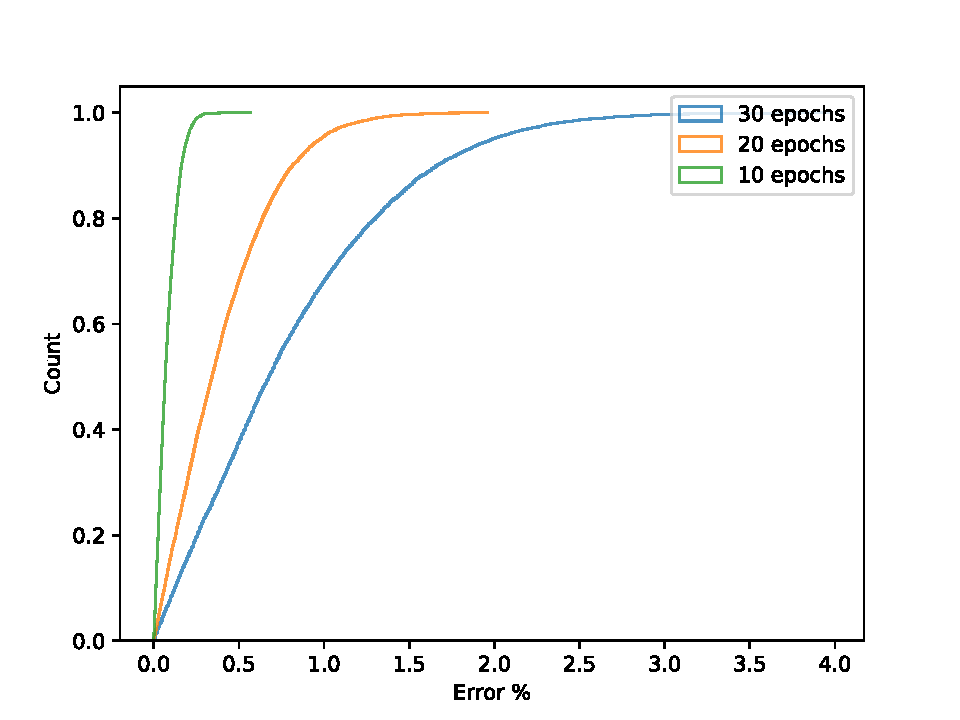
\includegraphics[width=0.9\linewidth]{results/microprofiling_dummy.pdf}
%  \end{subfigure}
%  \caption{Errors in accuracy prediction when using Microprofiling. Accuracy errors are higher when predicting for larger number of epochs, but still within xx\% of the true accuracy.}
%  \label{fig:multicam-cities}
%\end{figure}


% \section{Ekya Implementation}
\label{sec:system}

% impl overview

% logical integration

% key design choices
% - fine-grained gpu isolation
% - control interface with inference/retraining process
% - efficient support for microprofiling

%\junchen{this is copied from eval}
% We implement a prototype of \name using Python and the Ray framework~ \cite{ray}.

%Next, we describe how \name is integrated with existing libraries of DNN inference/training and the key design choices that optimize \name's efficiency in practice. 

% \subsection{API and integration}
% \label{sec:integration}

%\mypara{Interfaces}
%\junchen{1. what are the input API exposed by \name (sequence of images/frames); 2. what API does \name assume from the GPU library; and from the DNN runtime. 3. and importantly, these APIs are already provided by existing libraries and DNN inference/retraining can be done as is.}
%\name decodes video frames (images) from encoded video streams and feeds the frames to the inference tasks while also accumulating them to be used as input for the model's retraining at the beginning of each retraining window. 
% which are split into retraining tasks.
% Each task is a logical collection of data (images) accumulated in a retraining period. 
\name uses PyTorch \cite{pytorch} for running and training ML models. 
%Note that the training/inference jobs are logically the same as standalone training and inference tasks, so the underlying DNN engine can be seamlessly replaced and improved by better implementation.
%To allocate fractional GPU resources to each job, we need driver-level support from the GPU.
%\name uses Nvidia Multi-Process Service\cite{nvidia-mps} (MPS), which acts as a broker of GPU compute resources by intercepting CUDA calls and re-scheduling them according {\name}'s thief scheduler. 

\mypara{Modularization}
%\junchen{1. Instead of using a single top-down process, \name includes a collection of independent actors, each running the \name's control logic (microprofiling or thief scheduler or a training/inference job. 2. why? scalability? fault tolerance? slightly higher communication cost is tolerable since we operate on timescale of seconds.}
%While \name could be a single process, 
Our implementation uses a collection of logically distributed modules for ease of scale-out to many video streams and resources. 
Each module acts as either the \name scheduler, micro-profiler, or a training/inference job, and is implemented by a long-running ``actor'' in Ray \cite{ray}. 
A benefit of using the actor abstraction is its highly optimized initialization cost and failure recovery. %of training/inference models, thus allowing for % when they must be \gaa{invoked repetitively}, 
%Since an actor can keep a model loaded into GPU memory even when it fails, this allows for 
%quick recovery from failures. 
%\name also uses Ray to handle failures\junchen{Romil, add some details here}. 
% Moreover, this modularization allows Ekya to scale easily to multiple video streams and resources. Finally, actors are able to communicate in a peer-to-peer fashion, which allows training jobs to directly update the inference model when retraining completes.


\mypara{Dynamic reallocation of resources}% GPU isolation
\name reallocates GPU resources between training and inference jobs at timescales that are far more dynamic than required by prior frameworks (where the GPU allocations for jobs are fixed upfront ~\cite{kubernetes, yarn}).  
%There are two approaches to fine-grained GPU isolation for \name: (1) a middle layer, such as the Nvidia MPS~\cite{nvidiamps}, at the GPU driver level can reschedule GPU calls, or (2) dynamically throttling the per-process input load (such as reducing the video sampling rate) to ensure resources are freed up for use by others. 
While a middle layer like Nvidia MPS~\cite{nvidia-mps} provides resource isolation in the GPU by intercepting CUDA calls and re-scheduling them, it also 
%A middle layer like Nvidia MPS 
requires terminating and restarting a process to change its resource allocation. %, whereas throttling the load per-process may have the same effect without restarting the jobs, but Nvidia MPS enforces max-min fairness which does not allow arbitrary GPU partitioning. 
Despite this drawback, \name uses Nvidia MPS due to its practicality, while the restarting costs are largely avoided by the actor-based implementation that keeps DNN model in GPU memory. %\footnote{Currently, \name is limited to managing the GPU compute cycles. Extending {\name} to multiple resources like GPU memory is part of future work.%, and it assumes GPU memory is generally available. Processes today simply fail if they try to allocate more GPU memory than is available. However, 
%It is to be noted that recent work has shown that GPU memory can be virtualized with physical CPU memory \cite{salus, checkmate},and thus out-of-memory situations do not cause catastrophic failure. %In such a situation, GPU memory can be simply handled as an additional resource by \name.
%}
% For simplicity and fast model reloading, we use Nvidia MPS, but future work can consider regulating load as a mechanism to implement resource sharing.  
%\romil{This is not what we really do.. just mentioning it here based on discussion with Junchen.} \romil{Mention the default CUDA max-min fairness work?}


% \mypara{Placement onto GPUs} % GPU isolation
% The resource allocations produced by the thief scheduler are ``continuous'', i.e., it assumes that the fractional resources can be spanned across two discrete GPUs. To avoid the consequent expensive inter-GPU communication, \name first quantizes the allocations to inverse powers of two (\eg 1/2, 1/4, 1/8). This makes the jobs amenable to packing. \name then allocates jobs to GPUs in descending order of demands to reduce fragmentation \cite{tetris}. %, which ensures all jobs fit on the GPUs.


% \mypara{Model checkpointing and reloading}
% \name can improve inference accuracy by checkpointing the model {\em during} retraining and dynamically loading it as the inference model~\cite{tf-checkpoint, torch-checkpoint}.


% Checkpointing can, however, disrupt both the retraining and the inference jobs,
% so {\name} weighs the cost of the disruption (\ie additional delay on retraining and inference) due to checkpointing against its benefits (\ie the more accurate model is available sooner).
% Implementing checkpointing in \name is also made easy by the actor-based programming model that allows for queuing of requests when the actor (model) is unavailable when its new weights are being loaded. 


\mypara{Adapting estimates during retraining}
%{\name} relies on estimates on the expected accuracy from the retraining (to be explained in \S\ref{sec:profiling}), that it uses in Algorithm \ref{algo:thief_sched}. However, when the actual accuracy during the retraining varies from its expected value, {\name} reactively adjusts its allocations. 
When the accuracy during the retraining varies from the expected value from micro-profiling, {\name} reactively adjusts its allocations. 
%The {\em reactive} controller in {\name} (Figure \ref{fig:sys-arch}) monitors the growth in accuracy of the retraining jobs. 
Every few epochs, \name uses the current accuracy of the model being retrained to estimate its eventual accuracy when all the epochs are complete. It updates the expected accuracy in the profile of the retraining ($\Gamma$) with the new value, and then reruns Algorithm \ref{algo:thief_sched} for new resource allocations (but leaves the configuration that is used currently, $\gamma$, to be unchanged). 
%Since the increase in accuracy during the retraining is not always linear with the epochs, {\name} learns the {\em rate} of growth from prior retraining runs. %Further, to improve its estimation, {\name} also uses statistical techniques similar to those in prior work \cite{hyperdrive}.

%Ekya relies on offline profiles for estimating the expected final accuracy and completion time for each job. However, based on the input data, the performance of a model may vary from the expected profile. Ekya must adapt to any such variations.


%Ekya includes a reactive controller which continuously monitors the performance of training jobs and computes their deviation from the expected offline profiles. If the deviation crosses a fixed threshold, the job is immediately checkpointed and terminated and the profile is flagged as unreliable. \romil{Why not continue the job? Perhaps because its a bad use of resources?} If the profile is flagged as unreliable for 2 consecutive retraining windows, then it is allowed to run instead of being terminated, and the profile is updated with the newly observed curve. Thus, erring profiles are continuously updated while minimizing the cost from re-profiling correct profiles.


%\mypara{Batched micro-profiling}
% Microprofiling parallelization
% \junchen{1. why microprofiling needs speedup: while microprofiling reduces the total workload, it is still slow as it needs to test the configs one by one. 2. two optimizations: (a) sampled training data can be fit into memory once and reused; and (b) retraining can be parallelized}
%Micro-profiling, as explained in \S\ref{subsec:profiling}, can still be slow since it requires running multiple independent training jobs to get estimates for each configuration. 
%Since micro-profiling operates on the {\em same} (sub-sampled) data, \name loads the data to GPU memory once and reuses it for micro-profiling the different training configurations. In addition, these micro-profiling jobs can be parallelized and this parallelization also benefits from packing jobs together to maximize utilization~\cite{gandiva}.











% \subsection{Runtime enhancements in retraining window}
% \label{subsec:misc}

% \junchen{todo: 1. add thief scheduler acceleration, 2. maybe move checkpointing to a new implementation section}

% We next present two key enhancements to {\name} to improve its performance {\em during} the retraining of the jobs.

% \subsubsection{Checkpointing models.} 
% \label{subsubsec:checkpoint}





%\subsubsection{Decay factor} The inference accuracy of even the retrained model may {\em decay during the} retraining window because of shifting data distributions. While {\name} supports small retraining windows, we can also incorporate a decay factor (learned from history) in the {\sf\small Estim} module of \S\ref{subsec:thief}. 
%The inference accuracy of a retrained job is expected to decrease as the data distribution shifts over time. This is modeled in the profiles and incorporated in the simulator $S$ of the thief scheduler, which allows the thief scheduler to account for the eventual degradation of a retrainined model when deciding which cameras to prioritize. \romil{Not implemented}

%\noindent{\bf Retraining frequency.} The need for retraining depends on the changes in the data distribution. Some video stream may not require periodic retraining because their distributions may be stationary, while some video streams may change more rapidly, calling for a higher retraining frequency. This information is expected to be captured in the configuration profiles, where subsequent retrainings would demonstrate a lower accuracy gain. This information is directly consumed by thief scheduler which implicitly decides if a camera must be retrained or not by allocating resources. If a camera requires no retraining, the thief allocator will set it's resource allocation to 0. \romil{Add plots on the effects of retraining frequency} \ga{Add this to Section 2.1}

% \subsection{System Implementation}
% \romil{WIP}






%\section{Accuracy estimation with Microprofiling}
\label{sec:profiling}


% problem statement

% solution's principle - subset of data and configs

% subset of dataw

% config extrapolation (num. of epochs)

% prune out bad configs

% result teaser

% golden labels

% history-based alternate solution 


% profiling problem definition 
As shown in Figure \ref{fig:sys-arch} and explained in \S\ref{sec:solution}, {\name} relies on estimated accuracies of the retraining configurations for its scheduling decisions for each retraining window. Specifically, at the beginning of each retraining window $w$, the thief scheduler requires the estimated accuracy of each configuration $\gamma_v$, denoted as $a_v^{(w,\gamma)}$. The resource demands of the retraining configurations scale well with the size of the training data, and thus they only need to be measured once.

% Profiling
Predicting the accuracy of a fully trained model is challenging because it is dependent on the input data and stochastic training process. The problem is further compounded by the diversity in training configurations, which makes the training process unpredictable. However, as we show below, it is possible to predict the accuracy of a model within \romil{xx\%} if an initial seed knowledge of the model's training behavior is known. 

We simplify the accuracy prediction problem by training each configuration for a short duration on a sub-sample of the data. This micro-profiling process produces an accuracy value for each configuration when trained for a short duration on a subsample of the data. With each configuration's microprofiled accuracy as an input to the training loss curve model from \cite{optimus}, we can produce accuracy estimates for different epochs\romil{Add optimus model here}.

\cref{fig:microprofiling-bench} illustrates the effectiveness of micro-profiling in predicting model accuracy. We microprofile 6 hyperparameter configurations by training them for 5 epochs on 10\% data from a retraining window in the Cityscapes dataset. The accuracies produced by microprofiling are then used to estimate the accuracies if the model was trained without subsampling for 10, 20 and 30 epochs respectively. For comparison, we also train the same configurations for 10, 20 and 30 epochs without subsampling, indicated by the dotted curves. We see that \romil{...}

\romil{Talk about microprofiling cost/accuracy tradeoff?}

% Traditional hyperparameter tuning
Note that this problem different from the traditional hyperparameter tuning\cite{hyperband, asha}. Hyperparameter tuning involves picking the best performing configurations from a pool of candidate configurations, and thus can be modelled as a best-arm identification problem in a multi-armed bandit setting. It is implemented in a similar manner where multiple configurations are run in parallel and pruned as time progresses. However, our goal is not identifying the configuration which would yield the highest accuracy. We need to identify the training cost-accuracy tradeoff for each configuration such that the thief scheduler can make a globally optimal decision across configurations and video streams. Thus it is necessary to micro-profile each configuration instead of pruning configurations at runtime. 

{\bf Training labels.} Note that for the current retraining window as well as for the historical windows, {\name} acquires ``ground-truth'' labels using a golden model -- a high-cost but high-accuracy model pre-trained on a large dataset -- consistent with prior work \cite{incremental-13, mullapudi2019, incremental-15, distribution-20}. In every retraining window, {\name} runs the golden model on the training data to generate labels for retraining. We use the ResNet152 model trained on the MS-COCO dataset as our golden model. The cost of running the golden model is typically small (measured to be under $3\%$ of the retraining cost, as per our experiments).
% \romil{Add experiment to justify that golden model outputs are indeed representative of the ground truth}

\begin{figure}
  \centering
  \begin{subfigure}[t]{\linewidth}
    \centering
    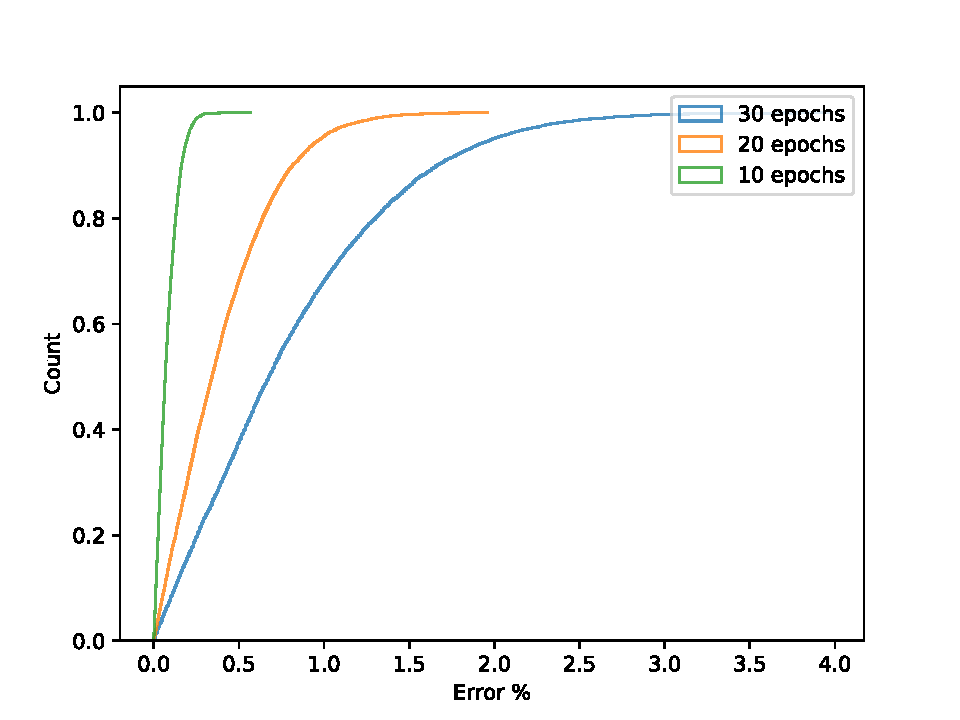
\includegraphics[width=0.9\linewidth]{results/microprofiling_dummy.pdf}
  \end{subfigure}
  \caption{\bf\small Errors in accuracy prediction when using Microprofiling. Accuracy errors are higher when predicting for larger number of epochs, but still within xx\% of the true accuracy.}
  \label{fig:multicam-cities}
\end{figure}


% 
\begin{figure*}[t]
\begin{subfigure}[b]{0.30\textwidth}
\centering
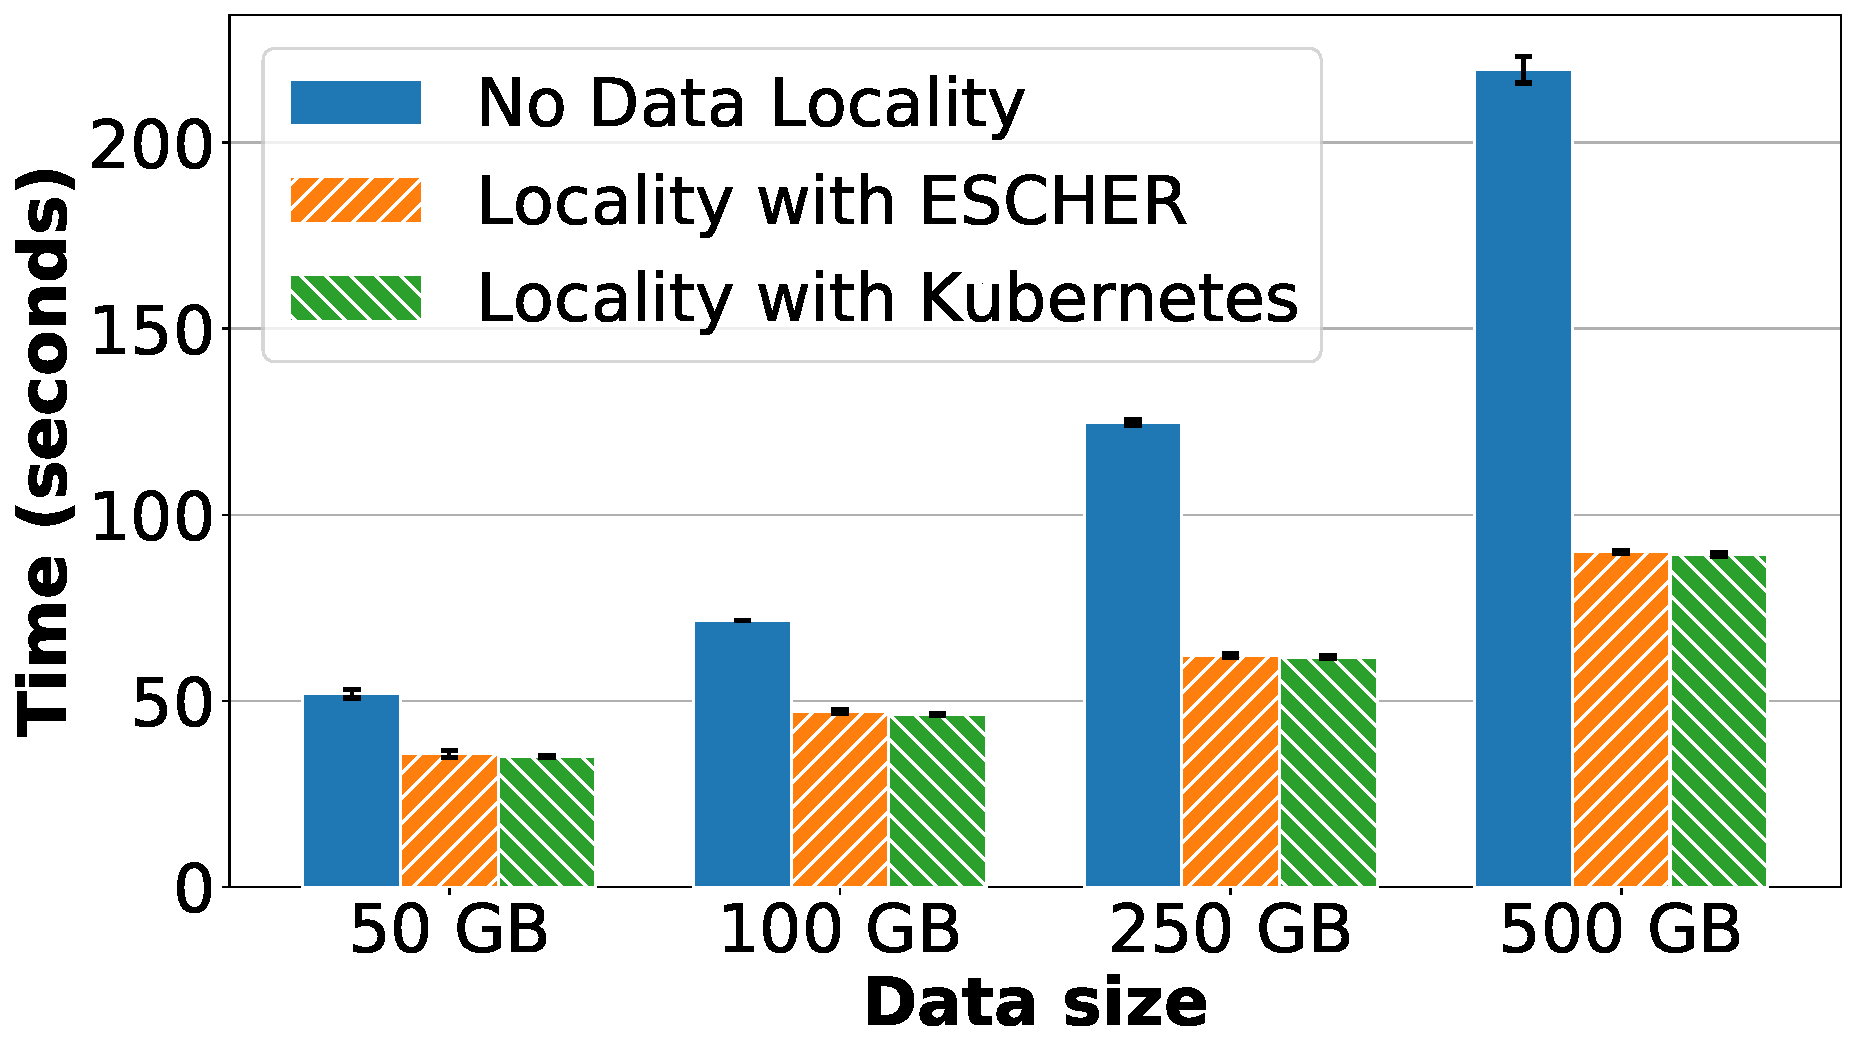
\includegraphics[width=\textwidth]{escher/plots/mapreduce_makespan.pdf}
\caption{
%A random placement policy has high network overheads due to poor data-locality. ESCHER implementation on Kubernetes performs comparably with the off-the-shelf core Kubernetes data locality policy.
}
\label{fig:mapreduce-makespan}
\end{subfigure}
\begin{subfigure}[b]{0.39\textwidth}
\hspace{2mm}
\footnotesize
% \begin{table}[ht]
% \begin{center}
\raisebox{15mm}{
\begin{tabular}{cccc}
% {\tiny
\toprule
& \multicolumn{3}{c}{\textbf{Scheduler}}\\
\textbf{Nodes}     & Generic & Kubernetes & ESCHER \\
\midrule
10 & $183.32 \pm 0.51$ & $54.69 \pm 0.46$ & $55.24 \pm 0.39$ \\\hline
50 & $113.71 \pm 0.49$ & $44.02 \pm 0.27$ & $44.71 \pm 0.44$  \\\hline
100 & $51.90 \pm 0.31$ & $35.08 \pm 0.31$ & $35.76 \pm 0.49$  \\
\bottomrule
% }
\end{tabular}
}
\caption{
% As the cluster size increases, ESCHER scales similarly to core kubernetes scheduler, while outperforming the generic data-locality unaware scheduler.
}
\label{tab:mapreduce-xnode}
%\vspace{-8mm}
% \end{table}
\end{subfigure}
\begin{subfigure}[b]{0.30\textwidth}
 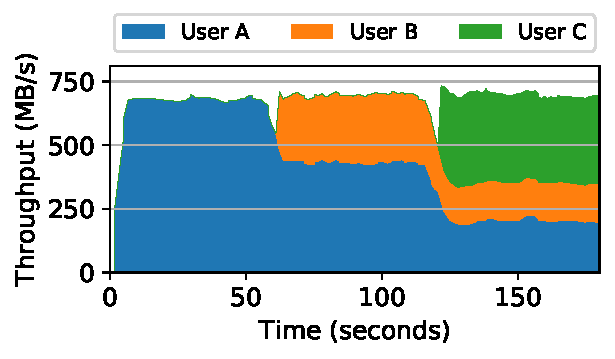
\includegraphics[width=\textwidth]{escher/plots/hfs/3user_hfs_sharing_mapreduce_50nodes_area_short.pdf}
 \caption{}
 \label{fig:hfs-3user-result}
\end{subfigure}
\vspace{-2em}
\caption{\small 
Data locality and hierarchical max-min fair sharing for WordCount.
\textbf{(a)} Makespan of WordCount running on a 100-node Kubernetes cluster, comparing a random placement policy, ESCHER on Kubernetes with data locality, and Kubernetes' native data locality.
\textbf{(b)} Makespan of WordCount MapReduce jobs in seconds across varying cluster sizes.
\textbf{(c)} Hierarchical max-min fair sharing with ESCHER.
A and B are in Sub-Org1 with weights 2:3; C is in Sub-Org2.
A, B, and C begin submitting tasks at $t=$0, 60, and 120, respectively.
}
\vspace{-3mm}
\end{figure*}


\section{Evaluation}
\label{sec:eval}

In this section, we evaluate the following questions:
\begin{compactitem}
    \item Can existing distributed applications be ported to use ESCHER and what are its implications?
    \item What are the tradeoffs with implementing scheduling policies in the application space vs in the framework?
    \item What are the overheads of scheduling with ephemeral resources?
\end{compactitem}

All evaluations use Amazon EC2 m5.12xlarge, m5.4xlarge or p3.8xlarge instances. Kubernetes clusters are provisioned using Amazon EKS running version 1.19.

\subsection{End-to-end Evaluation}
\label{sec:eval:e2e}
% Logical resources act as a thin layer of scheduling indirection for applications without sacrificing framework flexibility.
%In this section, we study four applications and their scheduling requirements. We then demonstrate how \name{} can accelerate these applications by allowing them to express complex scheduling policies with minimal developer effort.

\subsubsection{WordCount with MapReduce}
\label{eval:wordcount}
% What is mapreduce, what is word count
%These chunks are then individually processed by multiple mapper tasks in a distributed fashion. The results of mapper tasks are consumed by reduce tasks which key-wise consolidate the results.
WordCount counts the number of words in large text datasets and is often implemented with MapReduce~\cite{mapreduce}. To avoid expensive data transfers, data locality is essential.
% A data locality policy is essential to performance in this model, since map tasks must be colocated with their assigned inputs (which are usually on disk at a particular node) to avoid expensive data transfers.
% WordCount is a program implemented on the MapReduce~\cite{mapreduce} model to count the number of words in large text datasets. WordCount works by splitting the text file into smaller chunks, distributing them over the network and then running distributed mappers to count word frequency in these chunks.
% How data locality plays in. Implementation, HDFS Spark etc.
% The map tasks in WordCount are highly dependent on their locality with the data chunk they are assigned to process. If the data chunk is not present on the node where the map task is scheduled, it is forced to perform an expensive fetch over the network before starting processing. This dependence makes WordCount a benchmark to stress data-locality.
% Describe setup 100 nodes.
We implement the map and reduce tasks as independent operators running in containers.
The input files are chunks of a file with random words, each hosted by one of 100 nodes. The total input size is varied from 50 GB to 500 GB.
% and use Kubernetes to distribute these tasks over a 100-node cluster.
% The inputs are chunks of a file with random words, each  hosted by one of 100 nodes. 
% The total input size is varied from 50 GB to 500 GB.
%In this setup, the scheduler must place the mapper tasks on the nodes which host their chunk to minimize delays from network transfers.
We implement \name{} on Kubernetes, using an ESL for data locality (\Cref{policies}), and compare against Kubernetes's built-in data-locality policy~\cite{kubernetes-doc} and a locality-unaware random policy.
% For \name{} on Kubernetes, we use an ESL that implements data locality (\Cref{policies}).

% How do it in k8s, ESCHER.
% To achieve this data locality with the default Kubernetes scheduler, we use the \lstinline{NodeAffinityPriority} specifier in the scheduler to place mappers on nodes where their assigned chunk exists. This serves as a baseline to compares against ESCHER. In ESCHER, we create a resource \lstinline{chunk-n} on each node, where $n$ is the id of chunk hosted by the node. The mappers then request this resource to get co-located with their chunk. This policy is wrapped in an ESL which is invoked by WordCount.

Unsurprisingly, \Cref{fig:mapreduce-makespan} shows that as the input size increases, 
%the overhead of data transfer dominates execution if locality is not considered.
the overhead of transferring chunks over the network dominates the mapper computation time for the no-locality policy, taking up to 58.3\% of the total job time when the input size is 500 GB.
Meanwhile, \name{} on Kubernetes provides the same performance as Kubernetes itself, but without modifying the core scheduler framework.
Furthermore, \Cref{tab:mapreduce-xnode} shows that \name{} can also scale with the cluster size. 
%As the cluster size increases, the scheduling sub-system is stressed to distribute more map and reduce tasks.
Throughout different scales, ESCHER performs comparably with the core Kubernetes scheduler, with its makespan staying within $1.9\%$ of the baseline Kubernetes scheduler.. Implementing data locality with ESCHER required adding only two lines:  a \lstinline{set_resource} call during data generation to create a local \lstinline{data-<id>} resource and a line to specify a \lstinline{data-<id>} resource requirement for the mapper tasks.

% Compares against k8s
% Figure \ref{fig:mapreduce-makespan} and \Cref{tab:mapreduce-xnode} compare the makespan across different input and cluster sizes. % for a scheduling policy implemented in ESCHER, the off-the-shelf data-locality scheduler in Kubernetes and a policy which randomly places mappers without any data-locality.
% As the input size increases, the overhead of transferring chunks over the network dominates the mapper computation time for the no-locality policy, taking up to 58.3\% of the total job time when the input size is 500 GB.
% \Cref{fig:mapreduce-makespan} shows that ESCHER on Kubernetes can provide the same application-level benefits as Kubernetes itself, but without modifying the core scheduler framework.
% Furthermore, \Cref{tab:mapreduce-xnode} shows that as the cluster size increases, ESCHER can also scale with the increased number of map and reduce tasks (within $1.9\%$ of the core Kubernetes scheduler).

% As the cluster size increases, the scheduling sub-system is stressed to distribute more map and reduce tasks. Throughout different settings, ESCHER performs comparably with the core Kubernetes scheduler, with its makespan staying within $1.9\%$ of the baseline Kubernetes scheduler. 



% \begin{figure}
% \centering
% 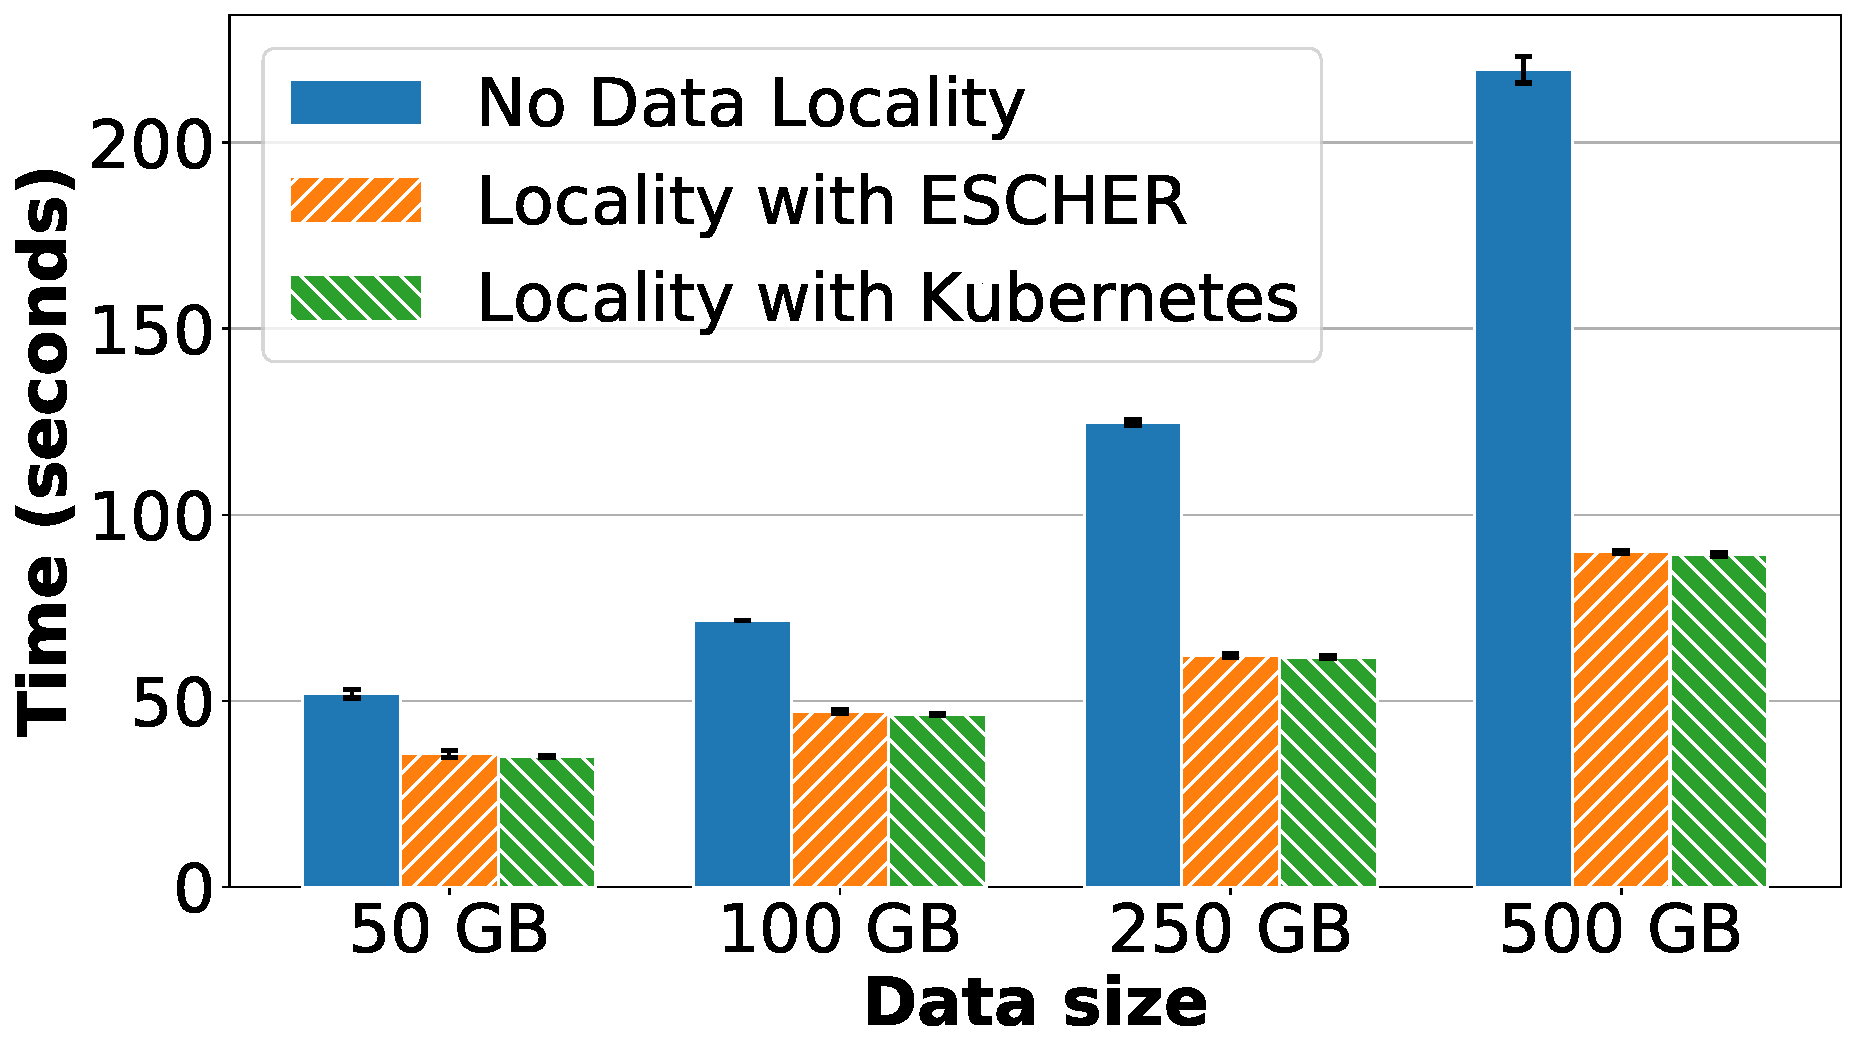
\includegraphics[width=0.8\columnwidth]{escher/plots/mapreduce_makespan.pdf}
% \caption{\small Makespan of WordCount running on a 100-node Kubernetes cluster, comparing a random placement policy, ESCHER on Kubernetes with data locality, and Kubernetes' native data locality.
% %A random placement policy has high network overheads due to poor data-locality. ESCHER implementation on Kubernetes performs comparably with the off-the-shelf core Kubernetes data locality policy.
% }
% \label{fig:mapreduce-makespan}
% \end{figure}

% \begin{table}[ht]
% \begin{center}
% \begin{tabular}{cccc}
% \toprule
% & \multicolumn{3}{c}{\textbf{Scheduler}}\\
% \textbf{Nodes}     & Generic & Kubernetes & ESCHER \\
% \midrule
% 10 & $183.32 \pm 0.51$ & $54.69 \pm 0.46$ & $55.24 \pm 0.39$ \\\hline
% 50 & $113.71 \pm 0.49$ & $44.02 \pm 0.27$ & $44.71 \pm 0.44$  \\\hline
% 100 & $51.90 \pm 0.31$ & $35.08 \pm 0.31$ & $35.76 \pm 0.49$  \\
% \bottomrule
% \end{tabular}
% \end{center}
% \caption{\small Makespan of WordCount MapReduce jobs in seconds, compared across varying cluster sizes.
% % As the cluster size increases, ESCHER scales similarly to core kubernetes scheduler, while outperforming the generic data-locality unaware scheduler.
% }
% \label{tab:mapreduce-xnode}
% %\vspace{-8mm}
% \end{table}


% \begin{figure}[ht]
% % \begin{subfigure}{1\linewidth}
% % \centering
% % 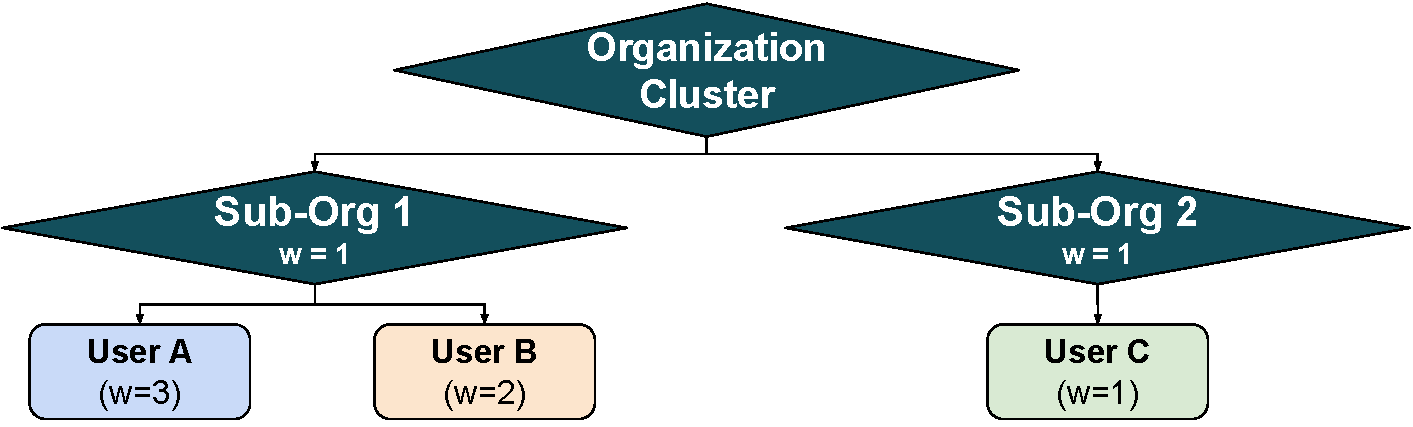
\includegraphics[width=1\columnwidth]{escher/plots/hfs/ESCHER_HFS_3User_OrgChart.pdf}
% % \caption{Organization Chart}
% % \label{fig:hfs-3user-orgchart}
% % \end{subfigure}
% % \begin{subfigure}{1\linewidth}
% \centering
% 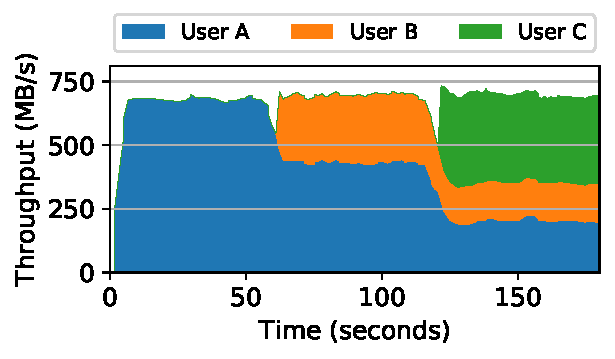
\includegraphics[width=0.93\columnwidth]{escher/plots/hfs/3user_hfs_sharing_mapreduce_50nodes_area_short.pdf}
% % \caption{User-wise throughput}
% % \end{subfigure}
% \caption{\small Per-user WordCount throughput with hierarchical max-min fair sharing.
% A and B are in Sub-Org1 with weights 2:3; C is in Sub-Org2.
% A, B, and C begin submitting tasks at $t=0,60,120$, respectively.
% %(a) shows the organization chart for resource sharing between sub-org 1 and sub-org 2. Weights (w) are relative to other users under the same parent.
% % (b) plots the throughput for users A, B and C on a cluster of 50 nodes.
% %At time t=0, only user A is submitting tasks so the HFS ESL allocates all resources to user A. At time t=60 and t=120, User B and User C start submitting tasks respectively.
% % The HFS ESLs adjust resource allocations based on utilization while maintaining organization level and sub-organization level weight proportional fairness.
% }
% \label{fig:hfs-3user-result}
% \end{figure}
% Two interfaces - infeasible and cancel tasks
% Throughput bug

% \begin{figure}
% \begin{subfigure}{1\linewidth}
% \centering
% 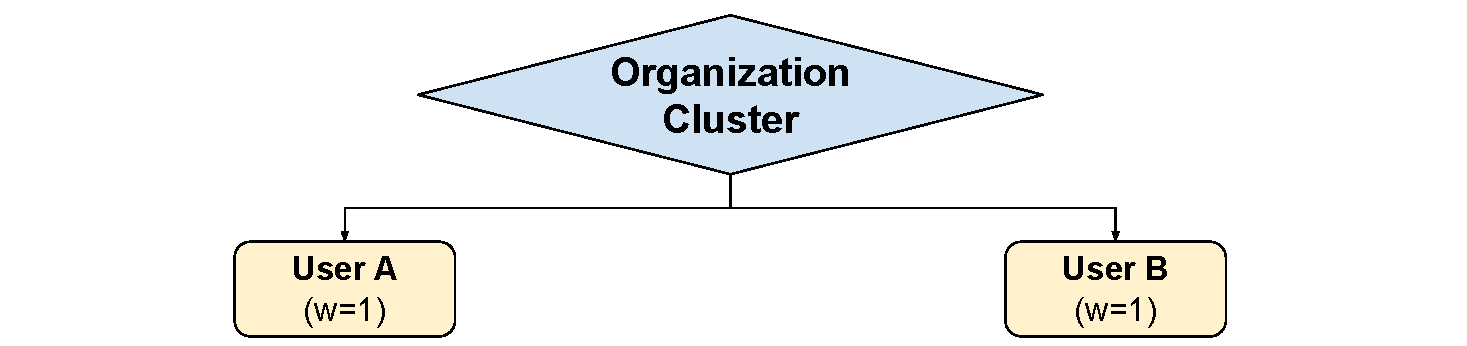
\includegraphics[width=1\columnwidth]{escher/plots/hfs/ESCHER_HFS_2User_OrgChart.pdf}
% \caption{Organization Chart}
% \label{fig:hfs-2user-orgchart}
% \end{subfigure}
% \begin{subfigure}{1\linewidth}
% \centering
% 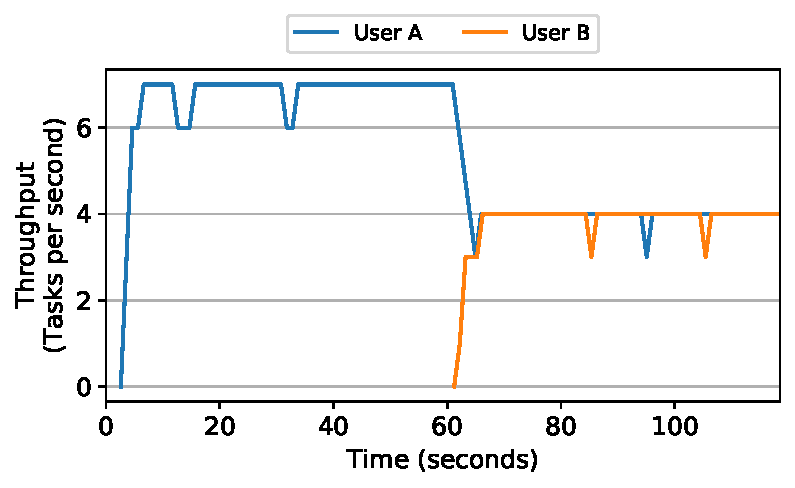
\includegraphics[width=0.9\columnwidth]{escher/plots/hfs/2user_hfs_sharing.pdf}
% \caption{User-wise throughput}
% \label{fig:hfs-2user-result}
% \end{subfigure}
% \caption{\small Min-Max Fair Sharing with ESCHER. Figure (a) shows the organization chart for resource sharing between User A and User B, each having equal weights (w=1). Figure (b) plots the throughput for users A and B. At time t=0, only user A is submitting tasks so the HFS ESL allocates all resources to user A. At time t=60 user B starts submitting tasks. The HFS ESL adjusts deallocates resources from user A and reassigns them to user B to maintain fairness.  
% }
% \label{fig:hfs-2user}
% \end{figure}

\subsubsection{Hierarchical max-min fair sharing}
\label{eval:hfs}
% Cool bits:
% \begin{itemize}
%     \item The resizing of the cluster is completely transparent to the users - they don't need to worry how many resources are allocated to them
%     \item Composition of data locality and fair sharing is as simple as adding resource requirements.
% \end{itemize}
Hierarchical Max-Min Fair Sharing (\Cref{policies}) allocates resources proportionate to a user's weight in a hierarchical organization.
% HFS maximizes resource utilization by reallocating idle resources.
Users submit jobs at different times, so their ideal absolute resource share is dynamic, making it impossible to maximize overall resource utilization with static labels.
% This makes it impossible to implement HFS with a static label-based scheduler since the resource share per user is dynamic.
For example, consider a two-team organization: Sub-Org1 with users A and B of weights 2:3, and Sub-Org2 with user C.
% with equal weights - Sub-Org1 and Sub-Org2. Sub-Org1 has two users, A and B with weights 2:3, while sub-org2 has one user C.
To ensure fairness with static labels, the only option is to allocate each user a fixed proportionate share, leading to under-utilization when only one user is submitting work.

% To achieve fairness, the only option with static labels would be to allocate each user a fixed share, leading to under-utilization in \Cref{fig:hfs-3user-result}. (i.e., A would only reach 200MB/s at $t$=0).

Because ephemeral resources can be \emph{dynamically} created and destroyed, an HFS policy ensures fairness while also maximizing overall utilization as users enter and leave the system~(\Cref{fig:hfs-3user-result}).
We deploy a HFS policy on a 100 node cluster running WordCount. We use a parent ESL for the teams and two children ESLs for Sub-Orgs 1 and 2 to create a hierarchy of ESLs.
An HFS ESL tracks idle resources and reallocates resources between teams or users.
% For example, at $t$=60 in \Cref{fig:hfs-3user-result}, B begins submitting tasks, causing the Sub-Org1 ESL to reclaim resources from A.
The workload in \Cref{fig:hfs-3user-result} starts with only user A submitting tasks to the scheduler. Since other users' resources are idle, the HFS ESLs re-allocate all idle resources to A to achieve max-min fairness. At time $t$=60, user B starts submitting tasks. This causes the Sub-Org 1 ESL to reclaim resources from A to re-allocate to B, in proportion to their weights. B's warmup time causes a small dip in net throughput at $t$=60. Finally at time $t$=120, user C starts submitting tasks and the parent ESL reallocates resources to Sub-Org2. Since Sub-Org 2 and Sub-Org 1 have equal weights, C's resource allocation is equal to the sum of A and B's allocation.
Ephemeral resources also enable composition: the application composes its custom policy (in this case, data locality for WordCount) with the two HFS ESLs by concatenating all the resource requirements.

% The workload in \Cref{fig:hfs-3user-result} starts with only user A submitting tasks to the scheduler. Since other users' resources are idle, the HFS ESLs re-allocate all idle resources to A to achieve max-min fairness. At time $t$=60, user B starts submitting tasks.
% This causes the Sub-Org 1 ESL to reclaim resources from A to re-allocate to B, in proportion to their weights. B's warmup time causes a small dip in net throughput at $t$=60. Finally at time $t$=120, user C starts submitting tasks and the parent ESL reallocates resources to Sub-Org2. Since Sub-Org 2 and Sub-Org 1 have equal weights, C's resource allocation is equal to the sum of A and B's allocation.

% Not only is ESCHER able to maintain the cluster's fair-sharing requirements, it also allows the each user to compose their application-level policies with cluster-level policies. This is achieved by simply concatenating the data-locality resources with the resource requirement vector from the fair-sharing ESL. This concatenation ensures that the scheduler places the tasks where both constraints - fairness and data-locality - can be satisfied.

% Using ephemeral resources also reduces implementation complexity by enabling transparent resizing of user shares when applying max-min fairness. Since the ESLs dynamically create and removes each user's ephemeral resources from underlying nodes, the users' applications are not required to keep a track of the resources allocated to them. This would not have been possible in a static label-based scheduler since the max-min shares for each user are dynamic. 



\subsubsection{AlphaZero}
AlphaZero \cite{silver2017mastering} is a reinforcement learning application for the board game Go.
%Unlike it's predecessor AlphaGo\cite{silver2016alphago}, AlphaZero does not require any human-generated training samples and can instead leverage reinforcement learning techniques to play and learn from games against itself.
%We base this experiment off an existing AlphaZero implementation \cite{anthony2017thinking}, which uses hard-coded process placement.
We demonstrate \name{}'s flexibility by porting an implementation~\cite{anthony2017thinking} onto Ray without compromising performance relative to the optimal hard-coded (but inflexible) placement.

AlphaZero executes a Monte Carlo Tree Search on the game state space in a CPU-intensive \textit{BoardAggregator} process. The search is guided by a \textit{PredictorAgent} running a neural network on a GPU which evaluates a board and predicts the associated reward.
%Based on this prediction, the \textit{BoardAggregator} generates new boards to explore and learn from.
% This pattern creates a tight feedback loop between the \textit{BoardAggregator} and the \textit{PredictorAgent}.
Co-locating \textit{BoardAggregator}s and their corresponding \textit{PredictorAgent}s on the same physical node is thus desirable to avoid network overheads from transferring board states. These pairings also require anti-affinity for load balancing and to avoid interference \cite{gandiva}.
%Many existing frameworks do not allow the expression of this composition of load-balancing and co-location policies, while others frameworks would require a tedious re-implementation of the scheduler. 
With ephemeral resources, this composed policy can be specified in 5 lines of code~(\cref{fig:alphazerocode}): we apply a load-balancing policy~(\Cref{tab:escher-constraints-policies}) to the \textit{PredictorAgent} and a co-location policy to the \textit{BoardAggregator} and \textit{PredictorAgent}.
%This composition takes only 5 lines of code (\cref{fig:alphazerocode}).

We ran 10k iterations of AlphaZero on a 32-node cluster (128 GPUs total). %board generation distributed across 16 machines with a total of 128 GPUs.
We compare three setups: 
(a) co-location with hard-coded placement,
(b) co-location with ephemeral resources, and 
(c) a baseline policy with no co-location. 
\Cref{fig:alphazerolatencycdf} plots the CDF for board exploration time. %, which includes generating the board on the \textit{BoardAggregator} and evaluating it on the \textit{PredictorAgent}. 
% Comparing the percentile distributions from this CDF in \cref{fig:alphazerolatencypxx}
Co-location is important for performance, outperforming no-colocation by 15.4\% in median latency and 20\% in P95 latency. %, demonstrating the benefits of co-location.
Additionally, co-location with ephemeral resources adds insignificant overheads of <1\%, while requiring less developer effort: the application code~(\Cref{fig:alphazerocode}) does not need to match \textit{PredictorAgent}-\textit{BoardAggregator} pairs to specific nodes.

% while providing a much simpler interface to express scheduling requirements.

%and by 714\% on P99.9 latency. P99.9 latency demonstrates the largest difference because the initial queries in the no-colocation case require setting up inter-machine communication sockets which may take time.

% Co-location with Logical Resources Stats - P999: 0.05949, P95: 0.02135, P50: 0.02083
% Static Co-location Stats - P999: 0.05863, P95: 0.02147, P50: 0.02079
% No Co-location Stats - P999: 0.06227, P95: 0.02578, P50: 0.02401


% \begin{figure}
% ~
% % Task co-location
% ~
% \begin{subfigure}{.22\textwidth}
%   \centering
%   \begin{minted}[fontsize=\tiny,breaksymbolleft=\tiny\ensuremath{},breakautoindent=true]{python}
% class PredictorAgent():
%   def __init__(id):
%     # Create resource for co-location
%     set_resource(label=id, capacity=1)
%     ...
%   \end{minted}
% \end{subfigure}
% ~
% % Task co-location
% ~
% \begin{subfigure}{.22\textwidth}
%   \centering
%   \begin{minted}[fontsize=\tiny,breaksymbolleft=\tiny\ensuremath{},breakautoindent=true]{python}
% class BoardAggregator():
%   def __init__(predictor):
%     # Assign predictor handle
%     self.predictor = predictor
%     ...
%   \end{minted}
% \end{subfigure}

% \newline

% \begin{subfigure}{.49\textwidth}
%   \centering
%   \begin{minted}[fontsize=\tiny,breaksymbolleft=\tiny\ensuremath{},breakautoindent=true]{python}
% def main():
%     # Create load-balancing resources
%     for node in cluster:
%         set_resource("load_bal", 1, node)
%     for i in range(0, num_agents):
%         p = PredictorAgent(resources = {"GPU": 1, "load_bal": 1}).launch(id=i)
%         # The predictor creates a resource with label i
%         # This resource is used by the BoardAggregator to co-locate.
%         b = BoardAggregator(resources = {i: 1}).launch(predictor=p)
%   \end{minted}
% \end{subfigure}
% \caption{AlphaZero placement preferences with \name{}}
% \label{figure:alphago}
% \end{figure}

\subsubsection{Distributed Training}
\label{sec:eval:tune}


% \begin{figure}
% 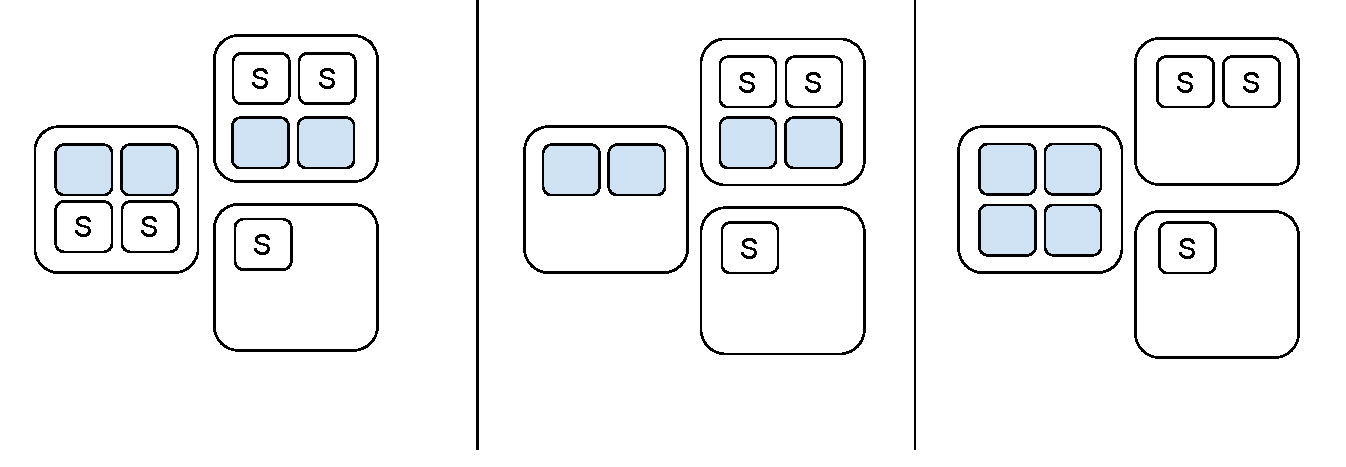
\includegraphics[width=0.9\columnwidth]{escher/figures/Eschertune.pdf}
% \caption{Migration after termination of the Short Job, signaling EscherTune to utilize a co-location mechanism and decrease communication overhead compared to Tune.
% }
% \label{fig:tune-results}
% \end{figure}



\def\longjob{\emph{long-job}}
\def\shortjobs{\emph{short-jobs}}
% Distributed training for a ML model typically consists of multiple workers that compute model updates in parallel and in lockstep.
For a distributed training job, worker placement is critical to performance, as co-locating workers reduces the cost of model synchronization at each step.
% The placement of these workers in a cluster is critical to the performance of the training process, as co-located workers avoid the network cost of model synchronization on each update operation.
%Typically, multiple jobs, each with different size and unpredictable completion time, will execute in parallel as part of a hyperparameter search~\cite{liaw2018tune}.
% Moreover, training jobs in a shared cluster can be of different sizes and with unpredictable completion times.
Gandiva \cite{gandiva} is a scheduler for deep learning jobs that aims to optimize training job performance. It composes a higher level \textit{load-balancing} policy and a lower-level \textit{co-location} policy to evenly spread jobs across machines while reducing intra-job communication overhead. 
To demonstrate \name{}'s flexibility, we augment Gandiva's \cite{gandiva} worker co-location and migration policy with Gang Scheduling to support distributed training jobs, and integrate the policy into Tune \cite{liaw2018tune}, an open source distributed training library built on Ray \cite{ray-osdi}, which we will refer to as \textit{EscherTune}.
We modified the Trial abstraction in Tune to be wrapped in a ghost task that ensures gang scheduling and applied co-location on tasks belonging to the same Trial.
%EscherTune records the current cluster placements during execution.
EscherTune triggers a migration whenever it detects sufficient available resources to place all workers of a job on the same node.
To execute a worker migration, EscherTune checkpoints the current job using application-specific checkpoint functionality and destroys all current workers. Then, EscherTune assigns ephemeral resources to the new target node, and relaunches all worker tasks of the training job without modifying their ephemeral resource requests.
 %To execute a worker migration, EscherTune will checkpoint the current training job using framework-dependent checkpoint functionality and destroy all current workers. Then, EscherTune assigns ephemeral resources to the target node and relaunches all worker processes of the training job with the specified ephemeral resource requests.
 
We compare EscherTune with Tune's open-source policy on a cluster of 12 GPUs. We launch 5 short-running training jobs (\shortjobs{}), each requiring 1 GPU, followed by 1 long-running training job requiring 4 GPUs (\longjob{}).
Each training job is training a ResNet-101 model on CIFAR-10 with a batch-size of 64 images per device.

Initially, the \shortjobs{} are load-balanced across the cluster, while the 4 workers of the \longjob{} are spread across the cluster depending on GPU availability. This is a sub-optimal placement, so EscherTune migrates the \longjob{} to colocate its tasks as soon as resources become available from a \emph{short-job} completion, resulting in 36.3\% higher throughput~(\Cref{fig:tune-results}).
Meanwhile, Tune uses a static placement, so the \longjob{}'s throughput remains the same.
% Figure \ref{fig:tune-results} compares throughput of \longjob{} in EscherTune and Tune, with all jobs launched at the same time. The throughput is low when the workers are spread across the cluster, but when there are sufficient resources to place workers on the same node, EscherTune is able to use ephemeral resources to migrate and co-locate all workers, increasing the throughput of the job by 36.3\%.
Furthermore, EscherTune's implementation consists of only 50 lines of Python, with no changes to Tune or the Ray scheduler. % a callback of 50 lines of Python, with \textit{no changes} to Tune.
 

% \begin{figure}[t]
% \centering
% 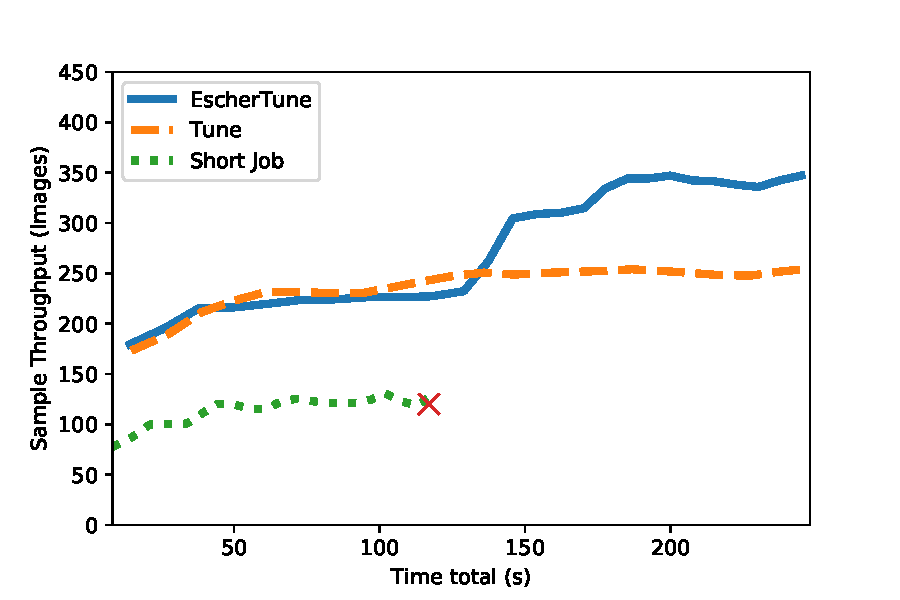
\includegraphics[width=0.85\columnwidth]{escher/plots/result_migrationthroughput.pdf}
% \caption{\small Throughput comparison of distributed training workloads with and without migration. ESCHER is able to augment an existing application, Tune, to increase sample throughput. 
% The red X indicates the termination of the short job, signaling EscherTune to utilize the co-location mechanism and decrease communication overhead compared to Tune.
% }
% % \caption{Throughput comparison of distributed training jobs with and without migration. 
% % Sample throughput for training can increase significantly by co-locating workers of
% % a distributed training job. In this mixed workload containing a distributed training job for a ResNet-101 architecture using 4 workers, ESCHER is able to easily augment the underlying framework to significantly improve performance. 
% % The red X indicates the termination of the Short Job, signaling EscherTune to utilize a co-location mechanism and decrease communication overhead compared to Tune.
% % }
% \label{fig:tune-results}
% \vspace{-0.3in}
% \end{figure}

% \subsubsection{Implementing Kube-Batch with ESCHER}
% To demonstrate ESCHER's ease-of-use, we add Gang Scheduling to Kubernetes using the Ephemeral Resources API and compare the implementation with a plug-in scheduler which adds this functionality to kubernetes. As described in Section \ref{sec:motivation}, adding gang scheduling to Kuberenetes in it's current form has been possible only through separate plug-in schedulers. One such plug-in is kube batch
\begin{figure*}[t]
\begin{subfigure}[b]{0.47\linewidth}
  \centering
\begin{subfigure}[t]{.22\textwidth}
  \centering
  \begin{minted}[fontsize=\tiny,breaksymbolleft=\tiny\ensuremath{},breakautoindent=true]{python}
class PredictorAgent():
  def __init__(id):
    # Create co-location resource.
    set_resource(
      name=id,
      capacity=1)
    ...
  \end{minted}
\end{subfigure}
~
% Task co-location
~
% \begin{subfigure}[b]{.21\textwidth}
%   \centering
%   \begin{minted}[fontsize=\tiny,breaksymbolleft=\tiny\ensuremath{},breakautoindent=true]{python}
% class BoardAggregator():
%   def __init__(predictor):
%     # Assign predictor handle
%     self.predictor = predictor
%     ...
%   \end{minted}
% \end{subfigure}
\begin{subfigure}[t]{0.72\textwidth}
  \centering
  \begin{minted}[fontsize=\tiny,breaksymbolleft=\tiny\ensuremath{},breakautoindent=true]{python}
def main():
  # Create load-balancing resources
  for node in cluster: set_resource("load_bal", 1, node)
  for i in range(0, num_agents):
    p = PredictorAgent(resources = {"GPU": 1, "load_bal": 1}).launch(id=i)
    # The predictor creates a resource with label i
    # This resource is used by the BoardAgg to co-locate.
    b = BoardAggregator(resources = {i: 1}).launch(p)
  \end{minted}
\end{subfigure}
  \caption{}
  \label{fig:alphazerocode}
\end{subfigure}
\begin{subfigure}[b]{0.26\textwidth}
  \centering
  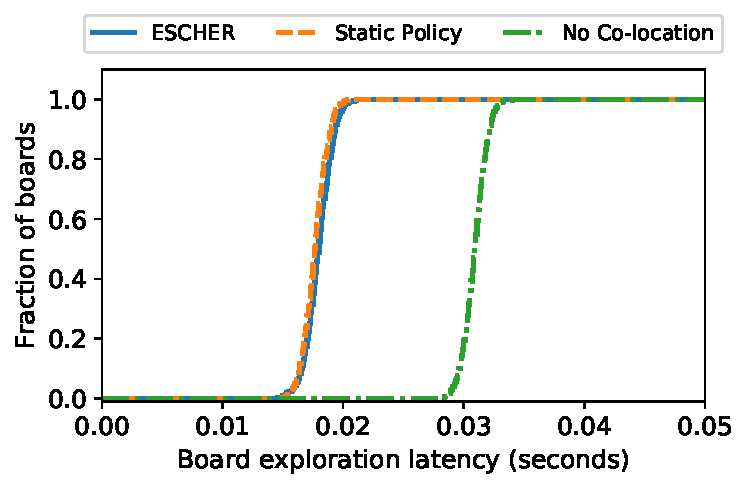
\includegraphics[width=\textwidth]{escher/plots/results_e2e_alphago_latencycdf_16node.pdf}
  \caption{}
  \label{fig:alphazerolatencycdf}
\end{subfigure}
\begin{subfigure}[b]{0.26\textwidth}
\centering
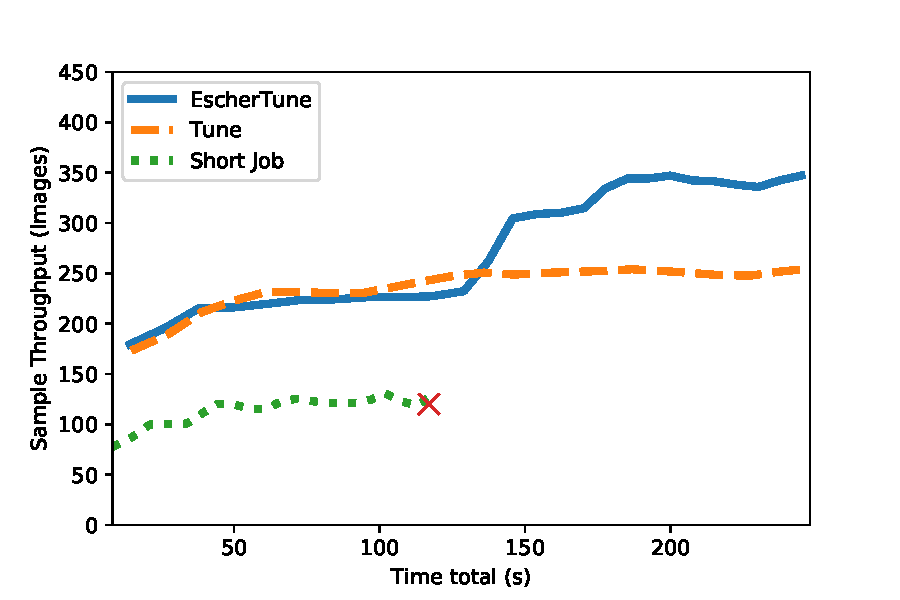
\includegraphics[width=\textwidth,trim=0cm 0cm 1.5cm 0cm, clip]{escher/plots/result_migrationthroughput.pdf}
\caption{}
\label{fig:tune-results}
\end{subfigure}
% \begin{subfigure}[b]{0.3\textwidth}
%   \centering
%   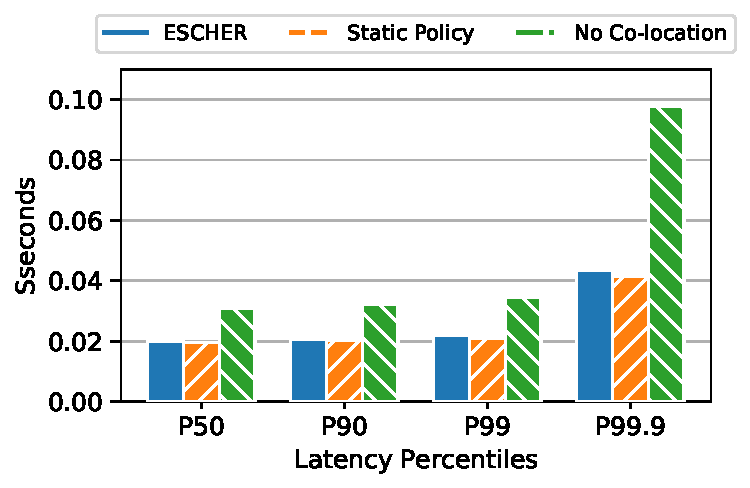
\includegraphics[width=\textwidth]{escher/plots/results_e2e_alphago_pxxcompare_16node.pdf}
%   \caption{}
%   \label{fig:alphazerolatencypxx}
% \end{subfigure}
\caption{\small AlphaZero and distributed training on \name{}. \textbf{(a)} Implementing AlphaZero policy with ESCHER, composing co-location with load-balancing.
% By co-locating the \textit{BoardAggregator}s and the \textit{PredictorAgent}s, the \name{} takes significantly lower time to generate and evaluate board states than an unaware scheduler. \name{} also performs comparably with a static policy that hard codes placement decisions, while offering the flexibility of a general scheduling policy.
\textbf{(b)} A CDF of AlphaZero board exploration latency, and
\textbf{(c)} Throughput comparison of a distributed training workload with a mix of short-running and long-running jobs. EscherTune is an augmentation of the hyperparameter search framework Tune~\cite{liaw2018tune}, using ESCHER to dynamically re-schedule jobs as others complete. %SCHER augments an existing application, Tune, to increase sample throughput. 
The red X indicates the completion of a short job. %, and EscherTune re-schedules the long-running job to claim the idle resources. % to utilize the co-location mechanism and decrease communication overhead compared to Tune.
}
\label{fig:alphazerolatencyfigure}
\vspace{-2mm}
\end{figure*}


\begin{figure}[t]
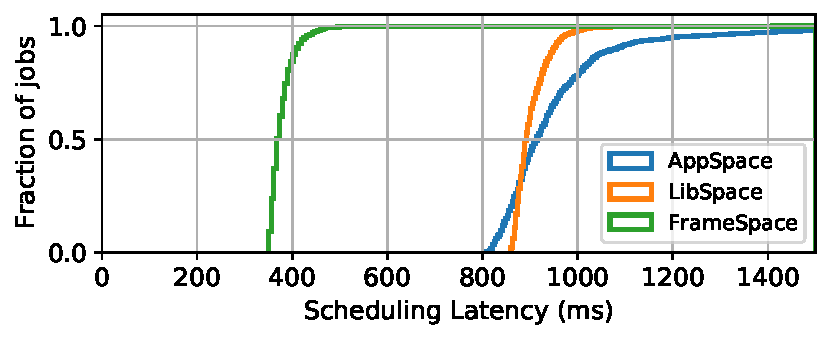
\includegraphics[width=0.92\columnwidth]{escher/plots/result_gangsched_design_compare.pdf}
\caption{\small Request latency for gang scheduling implemented in the application space, with (\textit{LibSpace}) and without (\textit{AppSpace}) coordination, versus the framework space (\textit{FrameSpace}). \textit{FrameSpace} is 1624 lines of code (LoC), \textit{LibSpace} with 261 LoC and \textit{AppSpace} with 78 LoC.}
\label{fig:gangscheddesign-results}
\end{figure}

\subsection{Microbenchmarks}
\subsubsection{Overhead of application-level policies}
\label{sec:eval:gangscheduling}
ESCHER scheduling policies can be implemented either in the application space for evolvability or in the framework for performance.
We evaluate the trade-offs involved in this choice by comparing three distinct designs of gang scheduling, all with ephemeral resources on Ray.

\textit{AppSpace} uses ghost tasks to atomically reserve resources (\Cref{policies:gangsched}).
% An application can call this policy without any coordination with another application in the same cluster.
While this policy is simple to integrate, the lack of coordination between applications can lead to deadlock, which must be resolved through timeouts. %it uses expensive ghost tasks to reserve resources and must resolve any livelocks through expensive timeouts.
\textit{LibSpace} avoids this by using a \emph{shared library}: a shared service in the cluster that serializes gang scheduling requests across applications.
% An application using \textit{LibSpace} sends all gang scheduling requests to this service, which returns the set of ephemeral resources that should be specified when submitting tasks.
\textit{LibSpace} thus avoids live lock entirely but requires deploying a separate shared service.
% \textit{LibSpace} improves upon this by using the same ghost task approach, but in a shared library which runs as a common service in the cluster to provide inter-job coordination. All jobs must communicate with this library to request gang scheduling of their tasks by specifying the resources required for scheduling all tasks. The library returns a ephemeral resource that must then be used by the application to place its tasks. \textit{LibSpace} is able to serialize gang scheduling across jobs, allowing it to avoid live-locks.
Finally, \textit{FrameSpace} modifies the Ray scheduler to expose a gang scheduling API.
Internally, a centralized service within Ray directly reserves and creates ephemeral resources.
Since it has direct access to the resource table, \textit{FrameSpace} avoids using ghost tasks, reducing overheads from worker allocation and task dispatch.

% implements gang scheduling as a part of the core Ray scheduler. This requires modifications in the core ray scheduler to expose an API for applications to request gang scheduling of their tasks. Internally, this implementation directly reserves resources in the scheduler's resource availability map and creates an ephemeral resource which is returned and requested by tasks to schedule their gang of tasks. 

\Cref{fig:gangscheddesign-results} compares the request latency of these designs on a 32-node cluster with 256 CPUs.
% We subsample 100k gang-scheduling requests from the Google ClusterData 2011 trace~\cite{clusterdata:Reiss2011}. % and measure the scheduling latency per request. %and measure the time taken from request submission to job start (scheduling latency).
% We subsample the Google ClusterData 2011 trace \cite{clusterdata:Reiss2011} to model request arrival patterns. 
% To evaluate the performance of these designs, we set up a cluster of 32 nodes with 8 CPUs each. We then submit 100k gang-scheduling requests over 15 minutes and measure the scheduling latency per request. %and measure the time taken from request submission to job start (scheduling latency).
% We subsample the Google ClusterData 2011 trace \cite{clusterdata:Reiss2011} to model request arrival patterns. Figure \ref{fig:gangscheddesign-results} compares the scheduling latency across the three designs.
While the mean latency of \textit{AppSpace} and \textit{LibSpace} is similar, \textit{AppSpace} has higher variance and a longer tail because it uses timeouts to break deadlocks.
\textit{LibSpace} incurs overhead from serializing requests at a separate service, resulting in a higher minimum latency. On average, \textit{FrameSpace} is nearly $2\times$ faster than \textit{AppSpace} and \textit{LibSpace} because it directly reserves resources instead of using ghost tasks. However, we note that for long-running tasks such as model training and batch processing workloads, the absolute scheduling latency is still a tiny fraction (<1s) compared to the runtime of the workloads (multiple hours). Moreover, implementing \textit{FrameSpace} is a significant effort, requiring a deep understanding of the Ray scheduler and modifying 1624 lines of Ray code.
To compare, \textit{LibSpace} and \textit{AppSpace} are implemented in 261 and 78 lines of \emph{application-level} code, respectively.



\subsubsection{Overheads of Ephemeral Resources}
% In this section, we evaluate the costs of introducing ephemeral resources in the framework scheduler.


%\textbf{Dynamic resource creation.}
%Scheduling with ephemeral resources relies on the ability to create and modify resources at run-time.
We evaluate the time to create resources and propagate their availability throughout the cluster.
Since the \lstinline{set_resource} call is asynchronous, we verify that the resources have been created and are available for use by launching no-op tasks that request these newly created resources. %The completion of these tasks marks the successful creation and propagation of ephemeral resources.
% \begin{figure}
%     \centering
%     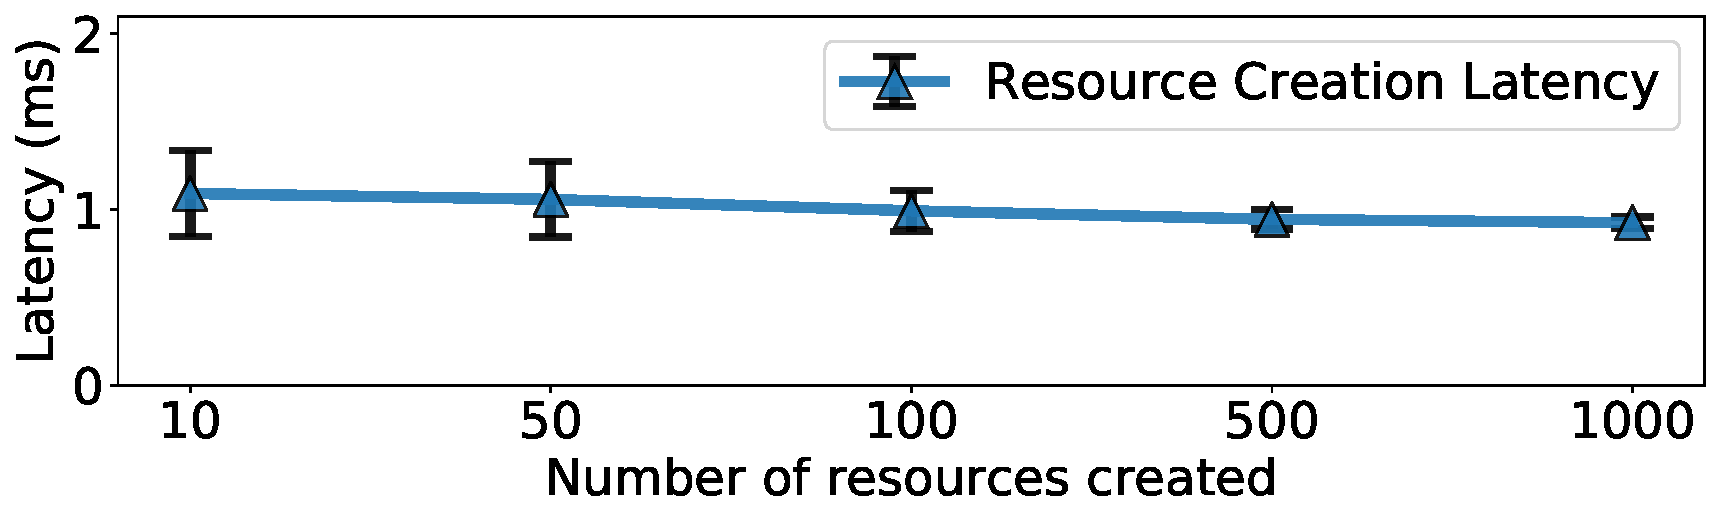
\includegraphics[width=\linewidth]{escher/plots/result_microbench_creationlatency_vs_numres.pdf}
%     \caption{\small Mean per-resource creation latency in Ray. Creating ephemeral resources in \name{} is a low cost operation that scales linearly with the number of resources created.}
%     \label{fig:res-creation-microbench}
% \end{figure}
Figure \ref{fig:res-creation-microbench} compares the mean latency of creating an equal number of resources on each node in a 50-node \ray{} cluster.
We show that even when creating 1000 ephemeral resources, we can maintain 1ms latency per request.
% against the number of resources created using the \lstinline{set_resource} API.
%Number of resources reflects the total resources created in the cluster, while the mean time to resource creation is measured as the time taken from the \lstinline{set_resource} submission to the availability of the resource.
As more resources are created, the cost of resource creation is amortized and the per-resource creation cost decreases to 0.72ms. 
In general, the overhead of creating or deleting an ephemeral resource should be roughly equivalent to that of a key-value store request.
% In absolute terms, the cost of creating ephemeral resources is insignificant, making \name{} a viable design.



\begin{figure*}[t]
\centering
\begin{subfigure}[b]{0.31\linewidth}
  \centering
  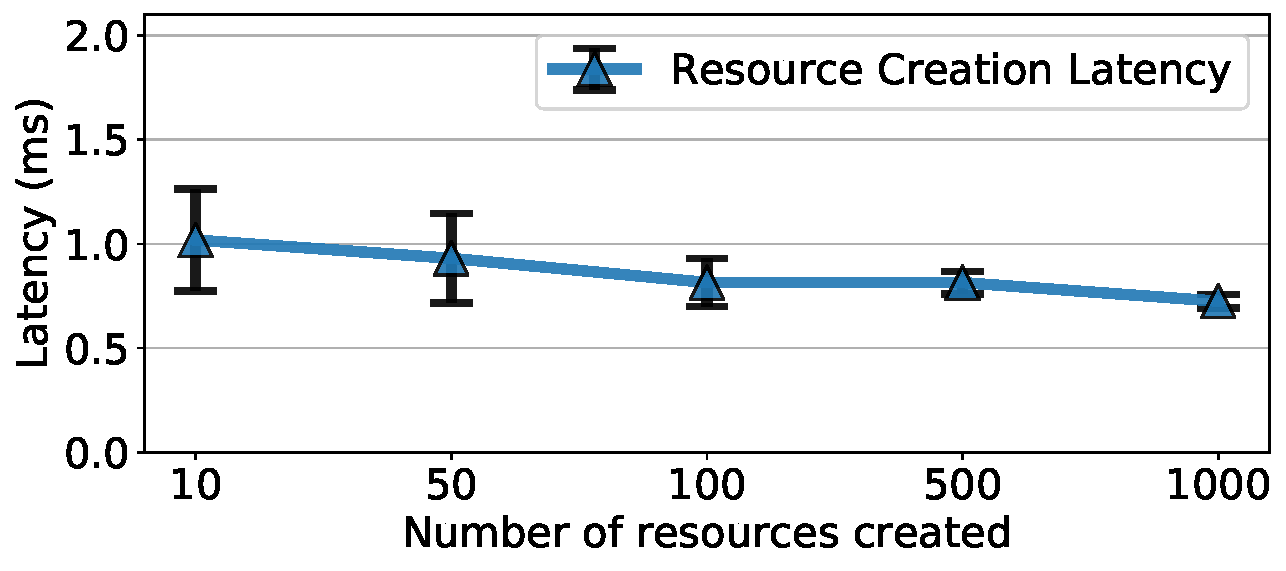
\includegraphics[width=\textwidth]{escher/plots/microbench_horz/result_microbench_creationlatency_vs_numres_horz.pdf}
  \caption{}
  \label{fig:res-creation-microbench}
\end{subfigure}
\begin{subfigure}[b]{0.31\textwidth}
  \centering
  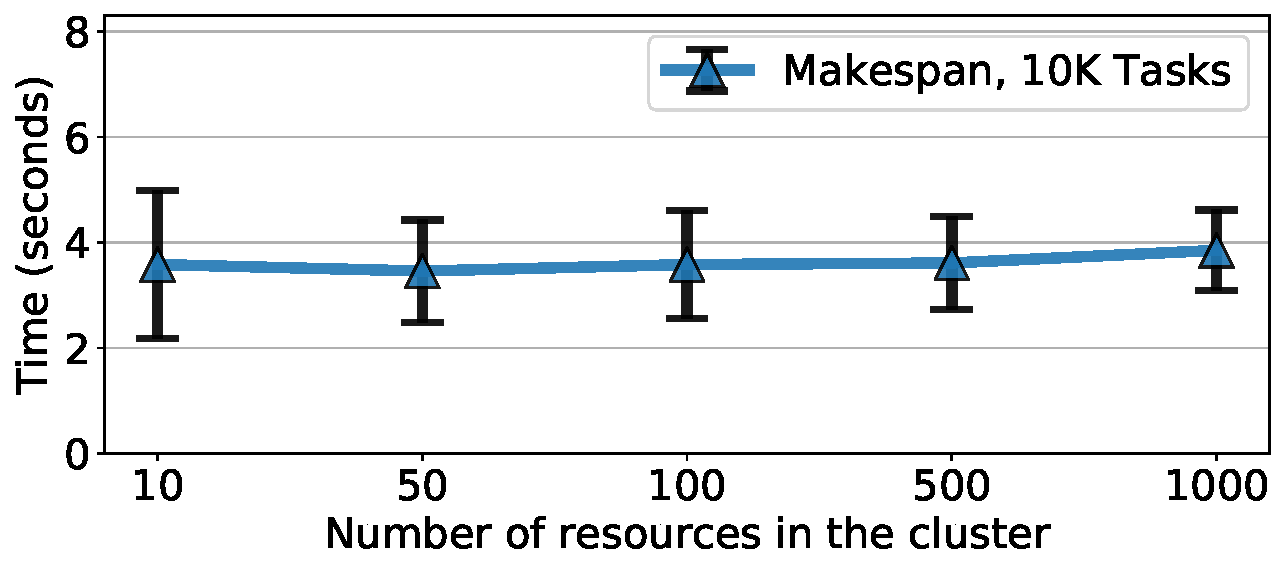
\includegraphics[width=\textwidth]{escher/plots/microbench_horz/result_microbench_schedlatency_vs_clusterresources_horz.pdf}
  \caption{}
  \label{fig:schedlatency-resources-microbench}
\end{subfigure}
\begin{subfigure}[b]{0.31\textwidth}
  \centering
  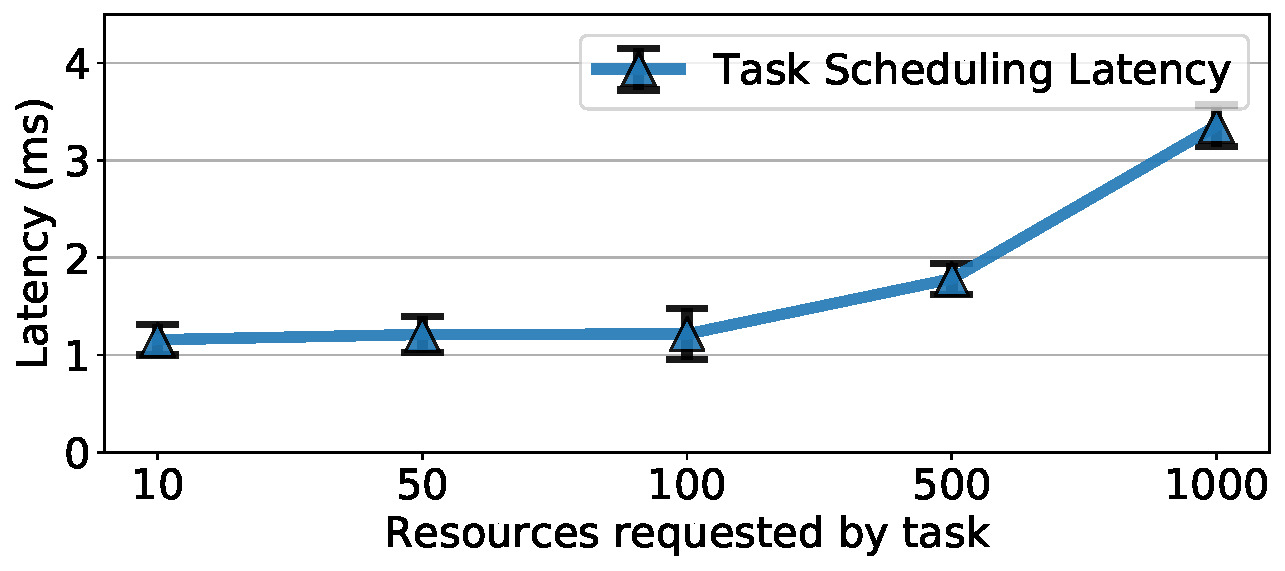
\includegraphics[width=\textwidth]{escher/plots/microbench_horz/result_microbench_schedlatency_vs_resrequested_horz.pdf}
  \caption{}
  \label{fig:schedlatency-taskrequest-microbench}
\end{subfigure}
\vspace{-4mm}
\caption{\small \name{} microbenchmarks. \textbf{(a)} Mean per-resource creation latency in Ray. Creating ephemeral resources in \name{} is a low-cost operation that scales linearly with the number of resources created. \textbf{(b)} Scheduling latency overheads from presence of ephemeral resources. Makespan of a 10000 task workload remains unaffected by the count of ephemeral resources in the cluster. \textbf{(c)} Effect of task resource requirements on scheduling latency in an environment with 10000 resources.}
\label{fig:microbenchfig}
\end{figure*}


\noindent\textbf{Ephemeral resources and scheduling latency.}
%The core task of the framework scheduler is to match task resource requirements with cluster resource availability.
The creation of ephemeral resources may add burden to the scheduler, as it must consider a greater number of attributes during resource matching.
% The usage of ephemeral resources imposes an additional burden on the scheduler and its resource matching complexity, as the number of resource attributes managed by the scheduler and the dimensionality of compared resource attribute vectors grows. 
Therefore, we analyze the effect of resource creation on task scheduling latency. We create an equal number of resources across 50 \ray{} nodes in a cluster using the \lstinline{set_resource} API. We then evaluate two cases based on the resource requirements of the tasks involved.

% \textbf{Tasks without resource requirements.}
First, in Figure~\ref{fig:schedlatency-resources-microbench}, we launch 10,000 tasks, none of which require any ephemeral resources to be scheduled. %, and measure the makespan of this workload against the number of resources present in the cluster.
As the tasks do not have any specific resource requirements, the scheduler execution time and workload makespan are not affected by the number of ephemeral resources present. %, and the makespan of the workload remains unaffected even by the presence of other ephemeral resources in the cluster.

% we highlight the effects of presence of ephemeral resources on scheduling latency for tasks that do not make use of ephemeral resources. In this microbenchmark, we launch a workload of 10k tasks, none of which require any ephemeral resources to be scheduled and compare the makespan of this workload against the number of resources present in the cluster. As the tasks do not have any specific resource requirements, the scheduler execution time remains constant, and the makespan of the workload remains unaffected even by the presence of other ephemeral resources in the cluster.
        % \begin{figure}
        %     \centering
        %     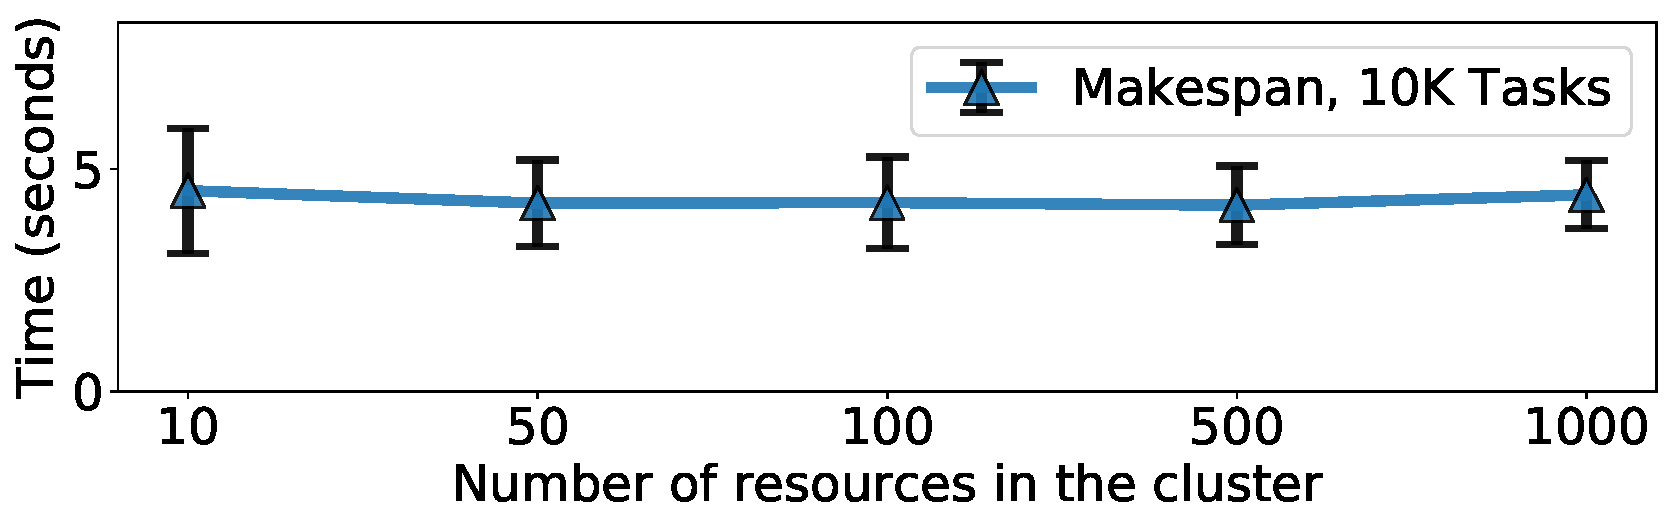
\includegraphics[width=\linewidth]{escher/plots/result_microbench_schedlatency_vs_clusterresources.pdf}
        %     \caption{\small Scheduling latency overheads from presence of ephemeral resources.  The makespan of a  10000 task workload remains unaffected by the count of ephemeral resources present in the cluster. }
        %     \label{fig:schedlatency-resources-microbench}
        %     \vspace{-4mm}
        % \end{figure}
        
% \textbf{Tasks with resource requirements.}
Second, when tasks do request ephemeral resources, the core scheduler must match the task's requirements to a set of candidate nodes.
To evaluate the overheads introduced by this matching, we setup a 50 node \ray{} cluster and create 1000 unique ephemeral resources evenly spread across nodes.
Figure 8c highlights the scalability of the scheduler as the number of ephemeral resources requested by a task grows. The the task scheduling latency grows only from 1.1ms to 1.2ms when requesting 1 vs. 100 ephemeral resources, respectively. We note that all policies described in this work require only a few ephemeral resources to express.
% We then perform multiple trials that launch a no-op task that requests a range from 10 to 1000 distinct resources.
%Figure \ref{fig:schedlatency-taskrequest-microbench} shows the scheduling latency of a no-op task against the number of resource requested by the task. The scheduling latency remains constant up to requests as large as 100 resources. Note that even the most complex scheduling policies do not require more than a few ephemeral resources.
    
        % \begin{figure}
        %     \centering
        %     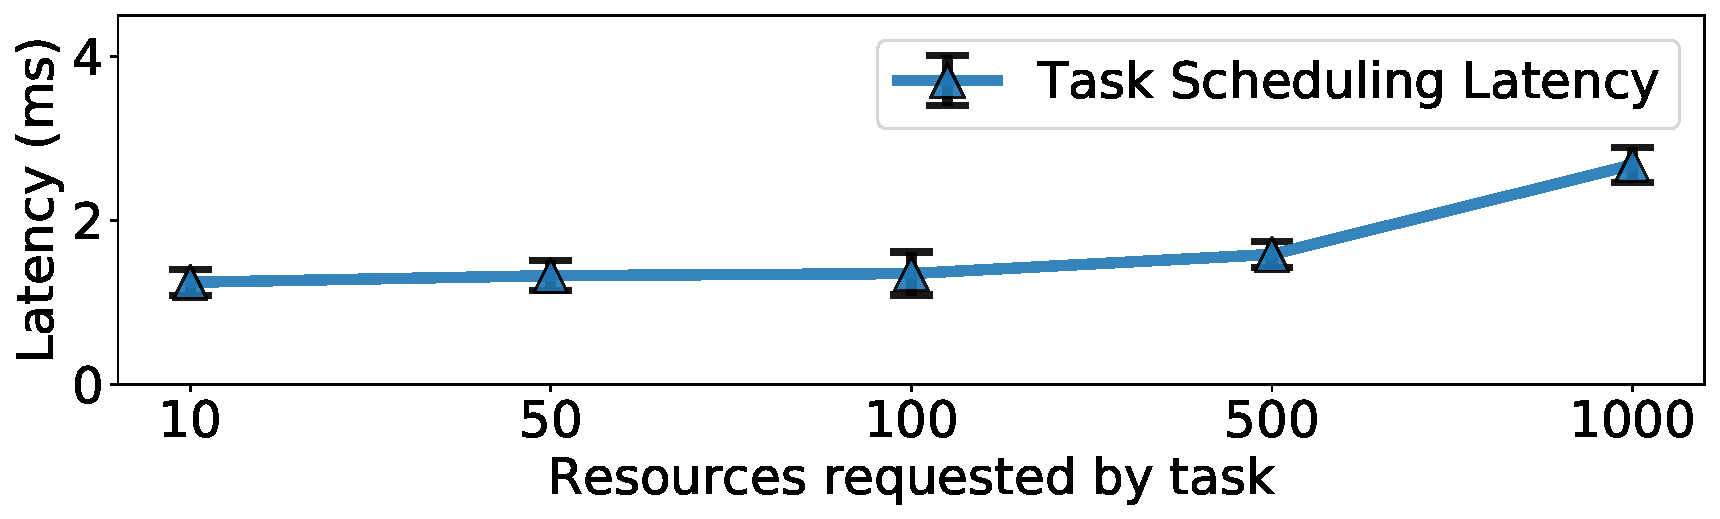
\includegraphics[width=\linewidth]{escher/plots/result_microbench_schedlatency_vs_resrequested.pdf}
        %     \caption{\small Effect of task resource requirements on scheduling latency in an environment with 10000 resources spread over 10 nodes. As a task resource requests more resources, the scheduling latency increases, but even the most complex scheduling policies do not require more than tens of resources. }
        %     \label{fig:schedlatency-taskrequest-microbench}
        % \end{figure}


% \textbf{Value of Locality-Aware scheduling.} In this microbenchmark, we study the motivation for co-location of tasks with the data they operate on. Specifically, we aim to evaluate the network cost of placing tasks and data on separate physical machines. We create arrays of varying sizes across 2 nodes in a \ray{} cluster and run two sets of tasks which fetch the data and perform a no-op. The first set of tasks uses ephemeral resources to co-locate with the data each task works on, while the other set of tasks is randomly placed.

% Figure \ref{fig:locality-latency} compares the task latency when tasks are co-located against random placement. \textcolor{red}{These numbers will be more dramatic soon - this run is local on one machine. Also, Is this a useful microbenchmark?}.

%     \begin{figure}
%         \centering
%         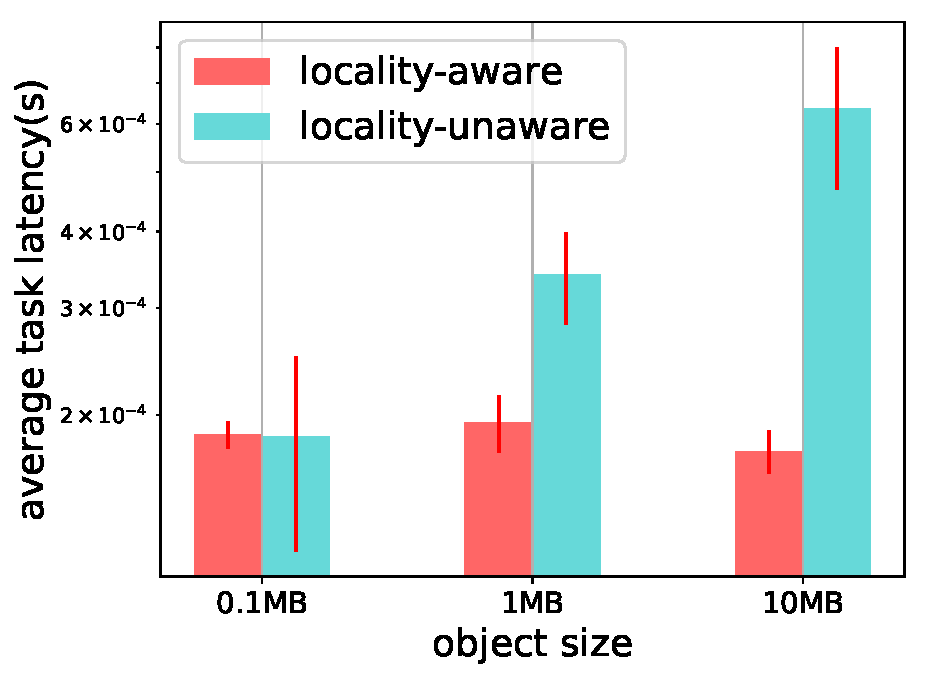
\includegraphics[width=\linewidth]{locality-latency.pdf}
%         \caption{Task-latency - Data-locality vs object size.}
%         \label{fig:locality-latency}
%     \end{figure}

% \subsection{Discussion}
% \textbf{Performance-evolvability tradeoff.} As we implemented our evaluation workloads, we found that \name{} significantly reduced the effort to express the workloads' scheduling constraints. In the AlphaZero workload, it required only 5 lines of code to be changed to express a composition of load-balancing and co-location. Implementing the same policy in Ray would have required re-writing the scheduler to enforce this policy on all tasks, since there is no policy selection mechanism in Ray. Same was true for implementing Gang Scheduling.

% However, as we see in the Gang Scheduling microbenchmark, the ghost task mechanism introduces latency due to the back-off performed by each ghost task on failure. While this latency is insignificant for long-running tasks, such as in distributed training, we acknowledge that this is a natural tradeoff ESCHER makes. It sacrifices performance for certain policies in favor of significantly reducing the implementation burden at the application-level. This gain in evolvability can be valuable for many applications, for whom functionality in the short-term (while the policy is integrated into the scheduler) may be more important than performance. 

% \textbf{Debugging ESCHER policies.} Since ephemeral resources are declarative in nature, debugging them requires replay of resource creation/deletion logs, which can be challenging.

% \section{Evaluation}
\label{sec:evaluation}

We evaluate \name{} on the Waymo and Cityscapes data. %The highlights are:

\begin{itemize}
    \item With multiple cameras sharing the resources on an edge server, \name{} achieves upto \romilc{16}\% \romil{This is sim, check exact with zhengxu} points higher accuracy than the fair sharing baseline. Attaining the same accuracy with a fair-sharing scheduler would require upto \romilc{$2.xx\times$} more resources.
    \item With the same resource provisioning, \name{} is able to support upto $5\times$ more video streams than the fair scheduler.
    \item \name{}'s performance gracefully degrades with reduction in resources to the baseline that does not retrain since it evaluates the cost of retraining on the accuracy. 
\end{itemize}

\subsection{Methodology}
\label{subsec:eval-setup}

\junchen{need to update}

\noindent\textbf{Datasets.} For our evaluation, we use the Waymo Open\cite{waymo} and Cityscapes\cite{cityscapes} datasets, two popular video datasets containing dashboard camera footage of cars driving through cities in the US and Europe. Cityscapes has frames from 27 video streams training with a total of 5000 pixel-level annotated frames, while Waymo Open has 1000 video segments with a total of 200000 frames.

The workload in Cityscapes is constructed by treating each city's video as an independent video stream feeding into {\name} for inference and retraining. The workload in Waymo Open is constructed by creating video streams by concatenating 20s-video segments belonging to the same city in chronological order. Each video stream in both datasets is then split into 10 retraining windows. These workloads are representative of independent video-streams with local variations which necessitate retraining for their specific data-distributions.



% \noindent\textbf{System Implementation.}\junchen{shrink or remove given the impl section}
% We implement a prototype of \name in Python using Ray\cite{ray} for asynchronous operations and RPCs. 
% Each video stream is modelled as an independent Ray actor whose resource allocation for inference and training is periodically updated by the Ekya master.

% % Write about microprofiling
% %\mypara{Microprofiling}
% The Ekya implementation ingests video streams and splits it into evenly sized retraining periods. At the start of each retraining period, the hyperparameters are micro-profiled \ref{sec:microprofiling} and the thief scheduler is run to compute the resource allocations for training and inference jobs. 
% %This resource allocation is then enforced by Ekya by launching new training processes and restarting the inference processes with updated resource weights. 

% Ekya requires fine-grained GPU allocation between inference and training processes. 
% Talk about memory isolation in Ekya.
% Talk about nvidia MPS resource sharing



\noindent\textbf{Trace driven simulator.}
% \junchen{update this?}
In addition to the system implementation \cref{sec:system}, we also built a simulator to simulate the execution of training and inference jobs under varying resource constraints and workloads. The inputs to the simulator are execution traces from training and inference workloads with different configurations. 

To collect execution traces, we ran all configurations in our hyperparameter space on the 10 retraining windows for every video stream in the Waymo and Cityscapes datasets. For each training job execution in a retraining window, we log the training-accuracy progression over GPU-time. Once the model is trained, we also log its test accuracy over the future retraining windows to get the accuracy in future windows if it was not retrained. This builds an exhaustive trace set that allows us to simulate custom scheduling policies, modify the execution order, simulate resource sharing and allocation. All profiling and trace collection was done on a testbed with Nvidia RTX 2080 and Intel Xeon E-2226G CPU.

% Talk about the assumptions - inference accuracy min GPU, linear scaling etc

\textbf{Hyperparameters.}
For each training job, we create a fixed set of configurations by varying the following hyperparameters - number of epochs to train, batch size, number of neurons in the last layer, number of layers to retrain, and the fraction of data between retraining windows to be used for retraining. We then selected combinations of these hyperparameters to create a diversity in the resource-accuracy profiles of the configurations. 

\mypara{Performance metrics}
\junchen{tbd: accuracy, throughput (\# of streams) under given \# of gpus}

\textbf{Baselines.}
We compare the thief scheduler against a weighted {Fair Scheduler} \cite{fair-1, fair-2, videostorm}, which allocates equal resources to all video streams and within a video stream, allocates resources to training and inference proportional to the weight set as the \lstinline{inference_weight} parameter to scheduler. A higher \lstinline{inference_weight} implies a higher resource allocation to inference and a reduced allocation to training jobs. To pick retraining hyperparameters, the fair scheduler employs the common heuristic of highest-accuracy first. 

%We compare against two baselines. First is \textit{No-retraining}, which does not ever retrain the model and thus allocates resources only to inference. Second is \textit{Fair Scheduler} \cite{fair-1, fair-2, videostorm} which allocates equal resources to all video streams and within a video stream, allocates equal resources to both, training and inference. To pick retraining hyperparameters, the fair scheduler employs the common heuristic of highest-accuracy first. 
% Why are these good baselines?

% \textbf{Metrics.}
% % More:
% Our most used metric is Inference Accuracy over time, as described in \S\ref{subsec:formulation}. We also use the number of GPUs provisioned at the edge server as a measure of cost.


% \junchen{

% 6.2 Overall improvement

% - accuracy vs. gpus (fix \# of videos)

% - streams vs. gpus (fix accuracy)

% - accuracy vs. streams (fix \# of gpus)

% - alternative architectures



% 6.3 Understanding Ekya improvements

% - ablation analysis

% - per-stream gains

% - temporal behaviors



% 6.4 Microbenchmarking

% - estimation accuracy of microprofiling

% - impact of microprofiling erros

% - delay of thief scheduler

% - impact of scheduling granularity


% }

% overall improvement: 
% acc vs gpu
% mention the cloud baseline
\subsection{Overall improvements}

\begin{figure}
  \centering
%   \begin{subfigure}[t]{0.5\linewidth}
%     \centering
%     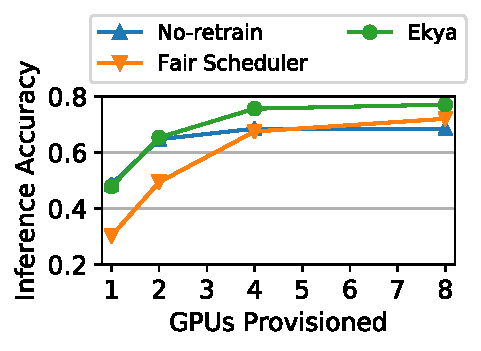
\includegraphics[width=\linewidth]{results/multicam/multicam_acc_vs_res_cityscapes.pdf} 
%     \caption{Cityscapes}
%     \label{fig:scalability-gpus-cityscapes}
%   \end{subfigure}
%   ~~~
%   \begin{subfigure}[t]{0.5\linewidth}
%     \centering
%     % \includegraphics[width=\linewidth]{figures/motivation/Class_Incrementality/class_distribution_change_sf_27.png}
%     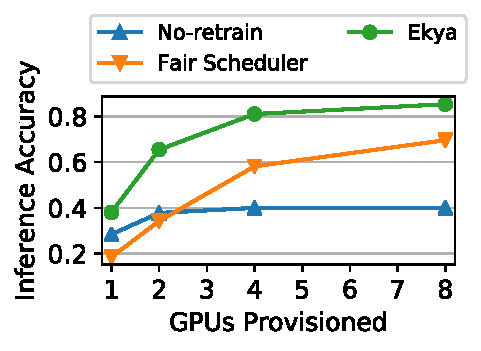
\includegraphics[width=\linewidth]{results/multicam/multicam_acc_vs_res_waymo.pdf}
%      \caption{Waymo}
%     \label{fig:scalability-gpus-waymo}
%   \end{subfigure}
  \begin{subfigure}[t]{0.5\linewidth}
    \centering
    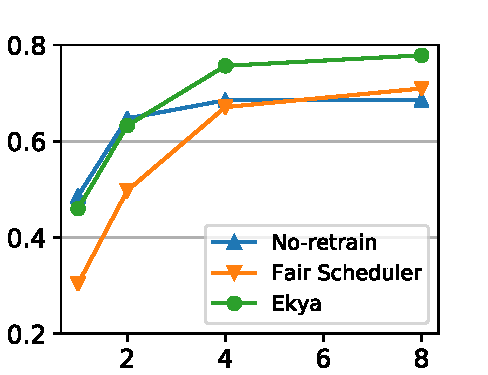
\includegraphics[width=\linewidth]{results/multicam/cityscapes_across_resources.pdf} 
    \caption{Cityscapes}
    \label{fig:scalability-gpus-cityscapes-golden}
  \end{subfigure}
  ~~~
  \begin{subfigure}[t]{0.5\linewidth}
    \centering
    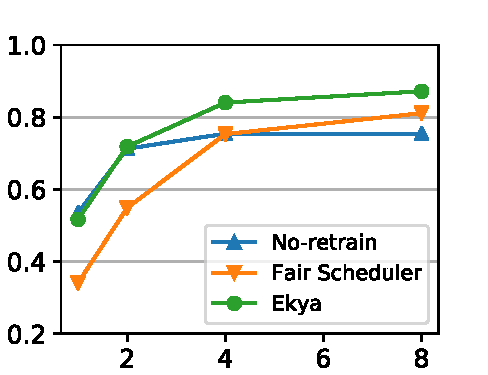
\includegraphics[width=\linewidth]{results/multicam/waymo_across_resources.pdf} 
    \caption{Waymo}
    \label{fig:scalability-gpus-waymo-golden}
  \end{subfigure}
  \caption{\bf Multi-video performance: Our accuracy gain over baselines increases with more GPUs. \romil{Set x,y axis labels and use the custom size params for matplotlib formatting. Reviewer Q.: How do you partition 10 video streams over 8 GPUs?}}
  \label{fig:scalability-gpus}
\end{figure}

\mypara{Accuracy vs. provisioned resource}
Figure~\ref{fig:scalability-gpus} compares the performance of \name, average inference accuracy under same amount of total GPU resource, with the no-retraining baseline and the fair-scheduler baseline.
In each of the Waymo and Cityscapes traces, we randomly pick 10 video streams and run their inference concurrently through five retraining windows.
As we increase the number of provisioned GPUs, we see that \name consistently outperforms the best of the two baselines by a considerable margin
\romilc{xx}\%-\romilc{xx}\% points higher accuracy in Cityscapes and \romilc{xx}\%-\romilc{xx}\% points in Waymo.
Note that these gains in accuracy are achieved without increasing inference delay.
\name allocates resource to retraining only when the accuracy gain from retraining the model outweighs the temporary accuracy drop due to frame subsampling, which explains why \name outperforms the no-retraining baseline. 
Moreover, when \name allocates resource to retraining, it allocates minimum amount needed by the retraining to finish in time, thus outperforming the fair scheduler.
While accuracy gap between \name{} and the fair scheduler baseline decreases as more GPUs are provisioned, \name needs much less resources (upto $6.5\times$ less GPUs, Table \ref{tab::resource-savings-golden}) to achieve the maximum accuracy that fair scheduler attains with 8 GPUs.

%\name's gains over no-retrain baseline are more sizable in Waymo than Cityscapes, but its gains over the fair scheduler baseline are comparable in both traces. 
%This suggests that Waymo data is inherently more suitable for continuous retraining, but through more intelligent resource allocation, \name can always squeeze more juice from retraining than fair scheduler.



% 
\begin{table}[t]
\small
\begin{tabular}{|c|c|c|c|c|}
\hline
\multirow{2}{*}{\begin{tabular}[c]{@{}c@{}}Video\\ Stream\end{tabular}} & \multirow{2}{*}{Accuracy} & \multicolumn{2}{c|}{GPUs Required} & \multirow{2}{*}{\begin{tabular}[c]{@{}c@{}}Resource\\ Savings\end{tabular}} \\ \cline{3-4}
                                                                        &                           & Ekya        & Fair Scheduler       &                                                                             \\ \hline
V0                                                                      & 76.6\%                    & 4           & 13.4                 & $3.3\times$                                                                 \\ \hline
V1                                                                      & 91.5\%                    & 4           & 4.9                  & $1.2\times$                                                                 \\ \hline
V2                                                                      & 78.1\%                    & 4           & 11.2                 & $2.8\times$                                                                 \\ \hline
V3                                                                      & 68.5\%                    & 4           & 14.9                 & $3.7\times$                                                                 \\ \hline
V4                                                                      & 66.9\%                    & 4           & 17.2                 & $4.3\times$                                                                 \\ \hline
V5                                                                      & 81\%                      & 4           & 6.4                  & $1.6\times$                                                                 \\ \hline
V6                                                                      & 80.9\%                    & 4           & 9.4                  & $2.3\times$                                                                 \\ \hline
V7                                                                      & 76.8\%                    & 4           & 15.1                 & $3.7\times$                                                                 \\ \hline
V8                                                                      & 67.8\%                    & 4           & 14.2                 & $3.5\times$                                                                 \\ \hline
V9                                                                      & 67.9\%                    & 4           & 8.9                  & $2.2\times$                                                                \\ \hline
\end{tabular}
\caption{Resource savings for different cities in Cityscapes.}
\label{tab:resource-savings-final}
\end{table}

\begin{table}[t]
\small
\begin{tabular}{|c|c|c|c|c|}
\hline
\multirow{2}{*}{\begin{tabular}[c]{@{}c@{}}Video\\ Stream\end{tabular}} & \multirow{2}{*}{Accuracy} & \multicolumn{2}{c|}{GPUs Required} & \multirow{2}{*}{\begin{tabular}[c]{@{}c@{}}Resource\\ Savings\end{tabular}} \\ \cline{3-4}
                                                                        &                           & Ekya        & Fair Scheduler       &                                                                             \\ \hline
V0                                                                      & 75.6\%                    & 4           & 15.6                 & $3.9\times$                                                                 \\ \hline
V1                                                                      & 78.6\%                    & 4           & 10.0                  & $2.5\times$                                                                 \\ \hline
V2                                                                      & 76.5\%                    & 4           & 19.5                 & $4.9\times$                                                                 \\ \hline
V3                                                                      & 74.5\%                    & 4           & 17.4                 & $4.4\times$                                                                 \\ \hline
V4                                                                      & 75.1\%                    & 4           & 20.9                 & $5.2\times$                                                                 \\ \hline
V5                                                                      & 71.4\%                      & 4           & 25.8                  & $6.5\times$                                                                 \\ \hline
V6                                                                      & 79.5\%                    & 4           & 8.05                  & $2.0\times$                                                                 \\ \hline
V7                                                                      & 75.3\%                    & 4           & 21.8                 & $5.5\times$                                                                 \\ \hline
V8                                                                      & 75.0\%                    & 4           & 84.5                 & $21.1\times$                                                                 \\ \hline
V9                                                                      & 75.2\%                    & 4           & 177.8                  & $44.5\times$                                                                \\ \hline
\end{tabular}
\caption{\bf\small Resource savings for different cities in Cityscapes. \romil{We should write DNF for V7 V8 V9. \romil{This is a bit confusing because every row is not running independently - so this isn't  per resource saving. We should either get overall aggregate number here or run V0 repeatedly to get per video number.}}}
\label{tab:resource-savings-golden}
\end{table}
% gains per stream
\mypara{Performance per video stream}
Figure~\ref{fig:multicam-cities} shows the improvements {\em per video stream} of \name over the baselines, using the same 10 video streams as in Figure~\ref{fig:scalability-gpus} when 4 GPUs provisioned. 
Rather than trading accuracies among video streams, \name re-allocates resources in a way that improves accuracy for {\em all} of the video streams. 
That said, the accuracy gain varies, with gains being more considerable on video streams that have low accuracy without retraining (no-retraining).
This is because these video streams tend to have more dynamic scenes thus may benefit more from retraining.
This highlights a desirable behavior of \name that resource will more likely to be assigned where more accuracy gains are expected.
% \junchen{again, any insight as to what might cause the difference between the two traces?}



% % temporal variance
% \mypara{Timeseries of \name performance}
% Figure~\ref{fig:multicam-timeseries} zooms in on one of the video streams from Figure~\ref{fig:multicam-cities} (V\fillme) and presents the timeseries of performance of \name and the baselines over the five retraining windows. 
% This is one of the video streams that see a high accuracy gain over no-retraining. 
% The timeseries corroborates our intuition: when no-retraining accuracy is low (the \fillme-th retraining window), \name allocates resource to allow it to retrain its model which keeps the accuracy at a high value.

% \begin{figure}
% 	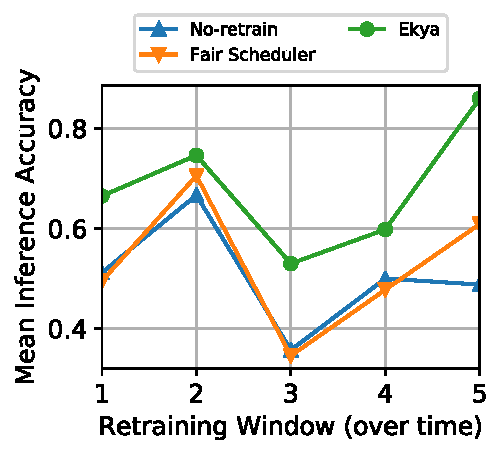
\includegraphics[width=0.4\textwidth]{results/multicam/multicam_taskwise_acc_zurich_4_cityscapes.pdf}
% 	\caption{\bf Timeseries of our performance vs. fair sharing. Again, adaptive resource sharing constantly outperforms fair sharing. \romil{Accuracy drops over time.}}
% 	\label{fig:multicam-timeseries}
% \end{figure}


% scalability: with more gpus, we can support more camera
\mypara{Scalability with more GPUs}
Next, we evaluate the scalability of \name's {\em throughput} as more GPUs are available.
We define throughput as the maximum number of video streams that can run concurrently on the GPUs while achieving a accuracy within a threshold of the maximum possible mean accuracy.
(This definition is common in practice, since applications usually require accuracy to be above a threshold for the inference to be usable.)
Figure~\ref{fig:scalability-gpu-vs-cam-thresholded} shows that \name's throughput grows almost linearly with more available GPUs, and at a rate \romilc{$2.3\times$} faster than the baseline of fair scheduler.
This suggests that \name can more easily scale to a large number of video sources than the baselines.

\begin{figure}
  \centering
%   \begin{subfigure}[t]{\linewidth}
%     \centering
%     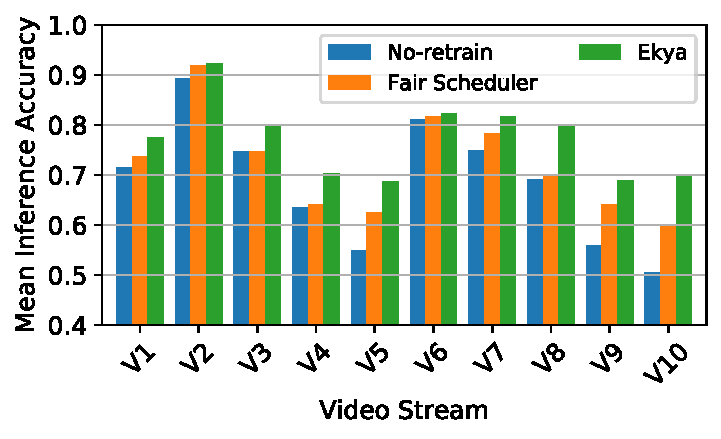
\includegraphics[width=0.9\linewidth]{results/multicam/multicam_individual_stream_acc_cityscapes.pdf} 
%     \caption{Cityscapes Human Label}
%     %\label{fig:multicam-cities-cityscapes}
%   \end{subfigure}
    \begin{subfigure}[t]{\linewidth}
    \centering
    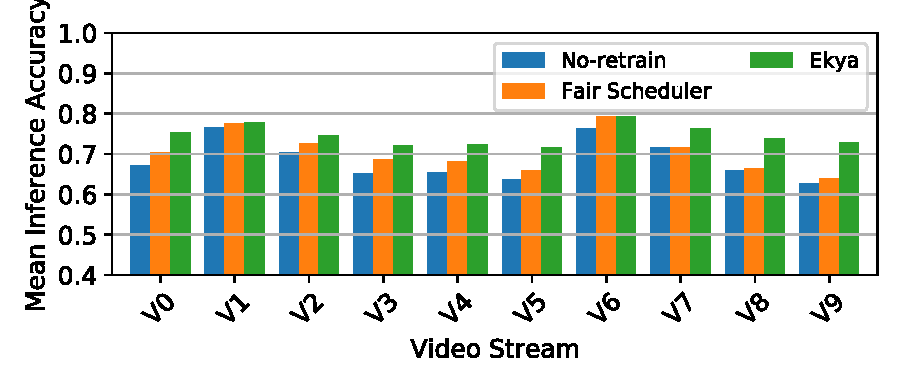
\includegraphics[width=0.9\linewidth]{results/multicam/cityscapes_across_cities.pdf} 
    %\caption{Cityscapes Golden Model}
    %\label{fig:multicam-cities-cityscapes}
  \end{subfigure}
%   ~~~
%   \begin{subfigure}[t]{0.5\linewidth}
%     \centering
%     % \includegraphics[width=\linewidth]{figures/motivation/Class_Incrementality/class_distribution_change_sf_27.png}
%     \includegraphics[width=\linewidth]{results/multicam/multicam_individual_stream_acc_waymo.pdf}
%      \caption{Waymo}
%     \label{fig:multicam-cities-waymo}
%   \end{subfigure}
  \caption{Multi-video performance: Ours (with continuous retraining) vs. Fair Share Scheduler. Compared across cities, we do consistently better. Some cities see bigger gains than others, which are thus prioritized by \name{}.}
  \label{fig:multicam-cities}
\end{figure}


Figure \ref{fig:scalability-fixedGPUs-accuracy} evaluates the throughput-accuracy tradeoff made by \name{} with a fixed number of resources. To minimize the accuracy variations between cities, we add video streams by replicating a fixed video stream from the Cityscapes dataset. 
With only a single GPU, increasing the number of video streams forces \name{} to gradually reduce resource allocation to retraining in favour of keeping of a high inference accuracy by allocating all resources to inference. The fair scheduler is unaware of the resource cost of retraining, and diverts GPU cycles from inference, resulting a lower inference accuracy.

\begin{figure}
 	%\includegraphics[width=0.4\textwidth]{figures/eval_placeholders/single-tradeoffs.pdf}
 	\includegraphics[width=\linewidth]{results/scalability/scalability_GPUs_cams_cityscapes.pdf}
	\caption{\bf Throughput measured as number of video streams that can be concurrently supported for different resource sizes subject to accuracy thresholds.
	%The accuracy threshold is a multiplicative factor of the maximum achievable mean accuracy for a workload given $\infty$ resources.
	}
	\label{fig:scalability-gpu-vs-cam-thresholded}
\end{figure}

% SIGCOMM Results:
% \begin{figure}
%  	%\includegraphics[width=0.4\textwidth]{figures/eval_placeholders/single-tradeoffs.pdf}
%  	\includegraphics[width=\linewidth]{results/scalability/scalability_cams_fixedGPUs_cityscapes.pdf}
% 	\caption{\bf Effect of adding more video streams on accuracy for different schedulers. When insufficient resources are provisioned, \name{} gracefully degrades to the No-retrain baseline, while the retraining decisions made by the fair scheduler reduce the mean inference accuracy.}
% 	\label{fig:scalability-fixedGPUs-accuracy}
% \end{figure}
\begin{figure}
 	%\includegraphics[width=0.4\textwidth]{figures/eval_placeholders/single-tradeoffs.pdf}
 	\includegraphics[width=\linewidth]{results/scalability/scalability_cams_fixedGPUs_cityscapes_golden_model.pdf}
	\caption{\bf Using golden model. Effect of adding more video streams on accuracy for different schedulers. When insufficient resources are provisioned, \name{} gracefully degrades to the No-retrain baseline, while the retraining decisions made by the fair scheduler reduce the mean inference accuracy.}
	\label{fig:scalability-fixedGPUs-accuracy}
\end{figure}


% per video. even if one video, gains are impressive
\mypara{Gains with single video stream}
Figure~\ref{fig:singlecam-cities} presents the same analysis of Figure~\ref{fig:scalability-gpus} but with only one video stream using the resources.
Across these video streams (and many others but not shown), we see that \name consistently outperforms the baselines by dynamically deciding when to retrain the model as well as the resource balance between retraining and inference.
As in Figure~\ref{fig:multicam-cities}, we see the gains vary considerably across video streams, which again highlights that some video streams can inherently benefit more from retraining.% their models.

% \begin{figure}
%   \centering
%   \begin{subfigure}[t]{\linewidth}
%     \centering
%     \includegraphics[width=\linewidth]{results/singlecam/singlecam_acc_vs_cost_cityscapes.pdf} 
%     \caption{Cityscapes}
%     \label{fig:singlecam-cities-cityscapes}
%   \end{subfigure}
%   \hfill
%   \begin{subfigure}[t]{\linewidth}
%     \centering
%     \includegraphics[width=\linewidth]{results/singlecam/singlecam_acc_vs_cost_waymo.pdf}
%     \caption{Waymo}
%     \label{fig:singlecam-cities-waymo}
%   \end{subfigure}
%   \caption{Single-video performance - different videos have different payoffs for retraining.}% In \ref{fig:singlecam-cities-cityscapes}, V2 demonstrates large benefits to retraining compared to V4.}
%   \label{fig:singlecam-cities}
% \end{figure}

\begin{figure}
  \centering
  \begin{subfigure}[t]{\linewidth}
    \centering
    \includegraphics[width=\linewidth]{results/singlecam/singlecam_acc_vs_cost_golden_cityscapes.pdf} 
    \caption{Cityscapes}
    \label{fig:singlecam-cities-cityscapes-golden}
  \end{subfigure}
  \hfill
  \begin{subfigure}[t]{\linewidth}
    \centering
    \includegraphics[width=\linewidth]{results/singlecam/singlecam_acc_vs_cost_golden_waymo.pdf}
    \caption{Waymo}
    \label{fig:singlecam-cities-waymo-golden}
  \end{subfigure}
  \caption{Single-video performance - different videos have different payoffs for retraining.}% In \ref{fig:singlecam-cities-cityscapes}, V2 demonstrates large benefits to retraining compared to V4.}
  \label{fig:singlecam-cities}
\end{figure}


\subsection{Comparison with alternative designs}
\label{subsec:eval-alternate}

Next, we evaluate two alternative designs for continuous retraining---(1) re-using a retrained model from a history window that shares class distribution (instead of retraining the model again) and (2) offloading the retraining to the cloud.

\mypara{Advantage over re-using cached models}
Reusing a cached model from history is tempting as it avoids the cost of model retraining. 
%Figure~\ref{fig:history-vs-current} compares 
We compare the accuracy of retraining the model on the current window (\name) with the accuracy of re-using the model from a history window in which the class distribution is close to the distribution in the current window (Euclidean distance $\leq 0.2$; \S\ref{sec:profiling}). Here we use ResNet18 as the model and Waymo as the trace.
%The graph, however, shows 
We observe that 
the accuracy is much lower by re-using the model from history, even when the history window share a similar class distribution. At median, the difference in accuracy is 11\% with the $90^\text{th}$ percentile and maximum divergence in accuracies being as high as $38\%$ and $51\%$. 
This confirms our intuition in \S\ref{sec:profiling} that although sharing a similar class distribution is indicative of the difficulty of retraining, it does not mean the model can be directly reused from any window with similar class distribution.


%\begin{figure}[t!]
%\centering
%\includegraphics[width=0.6\columnwidth]{figures/eval_placeholders/history-trained-vs-retrained-cdf.pdf}
%\vspace{-0.2cm}
%\caption{Gap between accuracy of the model retrained in the current and accuracy of re-using a model retrained in a history window that share similar class distribution.
%\vspace{-0.2cm}}
%\label{fig:history-vs-current}
%\end{figure}


\mypara{Advantage over a cloud-based solution}
Retraining could be offloaded to the cloud so the edge servers can focus on inference, but on a closer look such a cloud-based solution will even negate the benefit of retraining the model, because of the expensive communication delay from uploading training data to the cloud and downloading retrained models). 

%It is fundamentally challenging to run continuous learning across the edge-cloud because of network constraints.

% Math sheet new - https://docs.google.com/spreadsheets/d/1-WDeFmQwHy0sEpxL9f6QcbMKt1DVPaX6ODjMwDbb3IY/edit#gid=0
For instance, consider a setup serving 5 video streams in parallel with a retraining window size of 400 seconds. For a bit rate of 8 Mbps \cite{bitrate} and assuming a 10\% subsampling, it amounts to 320 Mb of training data being generated per camera in every retraining window. This retraining data must be uploaded to cloud and a model must be retrained and fetched back to the edge. Uploading 320 Mb over an average cellular uplink of 5.1 Mbps \cite{opensignal_2018} for 5 cameras results in a total upload time of 313 seconds. A model checkpoint of ResNet18 is 398 Mb, downloading which would take 23 seconds per camera on a downlink of 17.3 Mbps \cite{opensignal_2018}, or a total of 115 seconds for 5 cameras. The total network transfer cost is 428 seconds, which exceeds the retraining window size of 400 seconds. 

% Mention do we have to send everything to the cloud.

% examples where the drop is higher
Even on provisioning double the bandwidth (which entails an expensive change of the network link from cellular to cable), retraining on the cloud does not yield a higher accuracy in our simulator. We extend our simulator to simulate the network delays and assume that the the cloud offers a speed up of $10\times$ and has infinite parallel resources. Even then, the cloud \romilc{RTT} takes about 216 seconds and yields a mean inference accuracy of 81.8\%. In contrast, retraining at the edge completes in 125 seconds, leaving more time to take advantage of the retraining model, and results in an inference accuracy of 83.75\%.

% Show the calculation
% Mention the cost
% Varying network connections
Achieving the same accuracy in our simulations required increasing the downlink and uplink bandwidth by $3\times$ and still operates under the assumption that the cloud can provision parallel resources instantly, which can be expensive.

% Math sheet- https://docs.google.com/spreadsheets/d/1z4Zui8Qmg4iH-_yQKu7p0EZtXOlj_-ogKIW9mbf-Tpo/edit#gid=179811194

% For instance, each retraining window in the Waymo dataset accumulates about 1760 Mb of data every 20 seconds, resulting in a 88 Mb/s bitrate. Assuming a 10\% sub-sampling rate for retraining and a retraining window of 200 seconds (as in all our experiments), a total of 1760 Mb  of training data must be sent to the cloud. With an uplink of 5.1 Mb/s \cite{opensignal_2018}, just uploading the training data would take 345 seconds. Moreover, the updated model weights need to be downloaded from the cloud, which is 360 Mb in size. With a downlink throughput of 17.3 Mb/s \cite{opensignal_2018} (cellular connection), that adds another 20 seconds. Combined, this results in nearly 365s to get the retrained model, which far exceeds the retraining window size of 5 minutes (note that we have ignored the time to run the training in the cloud). Since even the sub-sampled video bitrate exceeds the limited bandwidths at the edge, this analysis applies for all retraining window sizes.


% \junchen{i still feel this should be in motivation section, no?}

\subsection{Sensitivity analysis}
\label{subsec:sensitivity-eval}

% \begin{figure} [t!]
%  	%\includegraphics[width=0.4\textwidth]{figures/eval_placeholders/single-tradeoffs.pdf}
%  	\includegraphics[width=\linewidth]{results/ablation_waymo.pdf}
% 	\caption{\bf {\name} factor analysis by removing  dynamic resource allocation and reducing the hyperparameter space.}
% 	\label{fig:factor-analysis}
% \end{figure}

\begin{figure} [t!]
 	%\includegraphics[width=0.4\textwidth]{figures/eval_placeholders/single-tradeoffs.pdf}
 	\includegraphics[width=\linewidth]{results/ablation_cityscapes_golden.pdf}
	\caption{\bf {\name} factor analysis by removing  dynamic resource allocation and reducing the hyperparameter space.}
	\label{fig:factor-analysis}
\end{figure}

% improvement breakdown
\mypara{Factor analysis}
To understand the contribution of each part of \name, we run a factor analysis on the same setting as Figure~\ref{fig:scalability-gpus} (10 video streams with 4 GPUs provisioned). We construct two schedulers from {\name}. \emph{Ekya-NoRes}, which removes the smart resource allocation in \name. \emph{Ekya-NoRes-NoEp} removes resource allocation and additionally fixes the number of epochs a model is trained to the maximum value, effectively removing it from the configuration space. We chose this hyperparameter for removal because it creates the largest diversity in the resource-accuracy profiles of configurations. 

As observed in Figure \ref{fig:factor-analysis}, the diversity in configurations and their careful selection has a large contribution to \name{}'s gains in accuracy when fewer resources are provisioned, which reduces as more resources are made available. This is because with more resources, even expensive configurations become feasible, thus configuration selection matters less. The smart resource allocation mechanism in {\name} has a nearly consistent contribution to \name{}'s performance.

%We note that the accuracy of \emph{Ekya-NoRes-NoEp} is lower than \emph{No-retrain} when 1 GPU is provisioned because resource reallocation is removed, and thus it always allocates resources to retraining. It just so happens that there are no good configurations to pick from once the epochs hyperparameter is removed, and thus the accuracy is lesser than \emph{No-retrain}.



% sensivity to accuracy errors
\mypara{Sensitivity to accuracy estimation errors}
\romil{Add paragraph and plot on accuracy of microprofiling.} %Resource consumption and accuracy of accuracy estimation. E
We now test the impact of errors in accuracy profiles (\S\ref{subsec:profiling}) on \name's performance gains.
To control the amount of errors, we add a controlled Gaussian noise on top of the real retraining accuracy as the predictions when the profiler is queried. 
Figure~\ref{fig:sensitivity-accuracy-error} shows that with upto 20\% errors in the profiler prediction, the maximum accuracy drop is 3\% points. When a 50\% profiling error is introduced, the accuracy drop is 7.9\% points. Such a large profiling error makes \name{} worse than the no-retrain baseline, but still better than fair scheduling.

\begin{figure}
	\includegraphics[width=\linewidth]{results/sensitivity/sensitivity_profileerrors_cityscapes.pdf}
	\caption{\bf Adding a controlled error $\epsilon$ to the accuracy prediction -  \name{}'s performance degrades, but only marginally.}
	\label{fig:sensitivity-accuracy-error}
\end{figure}

% Two subfigure plot for sensitivity 
% \begin{figure}
%   \centering
%   \begin{subfigure}[t]{0.5\linewidth}
%     \centering
%     \includegraphics[width=\linewidth]{results/sensitivity/sensitivity_profileerrors_cityscapes.pdf} 
% 	\caption{\bf Adding errors to the profiler.}
%     \label{fig:sensitivity-accuracy-error}
%   \end{subfigure}
%   ~~~
%   \begin{subfigure}[t]{0.5\linewidth}
%     \centering
%     % \includegraphics[width=\linewidth]{figures/motivation/Class_Incrementality/class_distribution_change_sf_27.png}
%     \includegraphics[width=\linewidth]{results/sensitivity/sensitivity_delta_acc_runtime_cityscapes_48gpu.pdf}
%      \caption{Effect of stealing parameter $\delta$ on the thief scheduler.}
%     \label{fig:sensitivity-delta}
%   \end{subfigure}
%   \caption{\bf Sensitivity Analysis Results.}
%   \label{fig:sensitivity-group}
% \end{figure}

% sensitivity to granularity
\mypara{Sensitivity to scheduling granularity} \ga{Change $\delta$ to $\Delta$ in the graphs and text.}
Finally, we show the sensitivity of \name to the allocation quantum $\delta$ (Algorithm \ref{algo:thief_sched}), which controls the runtime of the scheduling algorithm on the one hand and the result of the resource allocation on the other.
Figure~\ref{fig:sensitivity-delta} illustrates this tradeoff with the same setting as Figure~\ref{fig:scalability-gpus} (10 video streams with 4 or 8 GPUs provisioned).
Between $\delta=0.1$ and 1.0, higher $\delta$ reduces the runtime of the scheduler by 4$\times$, but the accuracy gain is severely affected. 
One should pick a higher $\delta$ only when the scheduler is relatively slow compared to a retraining window; otherwise, a low value of $\delta$ (fine-grained scheduling) is preferable.

\begin{figure}
  \centering
  \begin{subfigure}[t]{\linewidth}
    \centering
    \includegraphics[width=\linewidth]{results/sensitivity/sensitivity_delta_acc_runtime_cityscapes_48gpu.pdf}
  \end{subfigure}
  \caption{\bf Effect of the $\delta$ parameter on the thief scheduler. Larger values decrease the accuracy but are faster to compute.}
  \label{fig:sensitivity-delta}
\end{figure}

\subsection{System Implementation}
\romil{WIP}
\romil{Move this up in the implementaiton section and start with this result.}
The Ekya implementation is an end-to-end system which can ingest video streams and distribute retraining and inference jobs over a pool of shared GPU resources. We ran this implementation on our Edge test-bed \ref{machine-specs}. The load on the system was varied by changing the number of video streams that must be processed in parallel on the same pool of resources. \cref{fig:sysimpl-result} illustrates the performance of Ekya comapred against the fair scheduler for Cityscapes and Waymo datasets. Ekya offers a consistently higher accuracy than the fair baseline (by upto 8\% points) and Ekya can achieve the same accuracy as the fair scheduler, but support $2\times$ the number of video streams in parallel on the same set of resources.

Ekya's performance is affected by the runtime efficiency of it's scheduler. The thief scheduler's search over the resource-configuration space \ref{algo:thief_sched} can be computationally expensive, but relative to retraining window size, it is a small cost. As shown in \Cref{fig:sensitivity-schedlatency}, the t  hief scheduler computes a resource allocation for a retraining window of 200 seconds even when multiple GPUs must be allocated.

\begin{figure}
  \centering
  \begin{subfigure}[t]{\linewidth}
    \centering
    \includegraphics[width=\linewidth]{results/sensitivity/scheduler_resourcetime.pdf}
  \end{subfigure}
  \caption{\bf Thief scheduler latency for scheduling 10 video streams with varying available resource quantities and retraining period durations. The scheduler latency is a tiny fraction compared to the duration of the retraining period.  }
  \label{fig:sensitivity-schedlatency}
\end{figure}


\begin{figure}
  \centering
  \begin{subfigure}[t]{0.5\linewidth}
    \centering
    \includegraphics[width=\linewidth]{results/sys_impl/multicam_acc_vs_res_sysimpl_cityscapes.pdf} 
    \caption{Cityscapes}
    \label{fig:sysimpl-result-cityscapes}
  \end{subfigure}
  ~~~
  \begin{subfigure}[t]{0.5\linewidth}
    \centering
    \includegraphics[width=\linewidth]{results/sys_impl/sysimpl_varyingcities_waymo.pdf} 
    \caption{Waymo}
    \label{fig:sysimpl-result-waymo}
  \end{subfigure}
  \caption{\bf End-to-end accuracy on the system implementation on 1 GPU with varying number of cities.}
  \label{fig:sysimpl-result}
\end{figure}
\section{Implementation and Experimental Setup}
\label{subsec:eval-setup}

% \junchen{need to update}

\mypara{Implementation}
\name uses PyTorch~\cite{pytorch} for running and training ML models, and each component is implemented as a collection of long-running processes with the Ray\cite{ray} actor model. The micro-profiler and training/inference jobs run as independent actors which are controlled by the thief scheduler actor. \name achieves fine-grained and dynamic reallocation of GPU between training and inference processes using Nvidia MPS~\cite{nvidia-mps}, which provides resource isolation within a GPU by intercepting CUDA calls and rescheduling them. Our implementation also adapts to errors in profiling by reactively adjusting its allocations if the actual model performance diverges from the predictions of the micro-profiler. \name's code and datasets are available at the project page: \href{https://aka.ms/ekya}{aka.ms/ekya}

\mypara{Datasets} 
We use both on-road videos captured by dashboard cameras as well as urban videos captured by mounted cameras. The dashboard camera videos are from cars driving through cities in the US and Europe, Waymo Open~\cite{waymo} (1000 video segments with in total 200K frames) and Cityscapes~\cite{cityscapes} (5K frames captured by 27 cameras) videos. The urban videos are from stationary cameras mounted in a building (``Urban Building'') as well as from five traffic intersections (``Urban Traffic''), both collected over 24-hour durations. % and a set of 24-hour urban traffic videos (``Urban Traffic'') captured by 5 cameras. %\junchen{add bellevue dataset once it's included}
% For our evaluation, we use the Waymo Open\cite{waymo} and Cityscapes\cite{cityscapes} datasets, two popular video datasets containing dashboard camera footage of cars driving through cities in the US and Europe. Cityscapes has frames from 27 video streams training with a total of 5000 pixel-level annotated frames, while Waymo Open has 1000 video segments with a total of 200000 frames.
We use a retraining window of 200 seconds in our experiments, and split each of the videos into 200 second segments.  
%The traffic videos are captured continuously and we split them into 200-second retraining windows. 
Since the Waymo and Cityscapes dataset do not contain continuous timestamps, we 
%However, the two public datasets %organize their images chronologically but 
%do not contain continuous timestamps.We 
create retraining windows by concatenating images from the same camera in chronological order to form a long video stream and split it into 200 second segments. %10 retraining windows. 
% in Cityscapes, treating a block of consecutive \fillme images from the same video source (in total 27 sources); and (2) in Waymo, concatenating 20s-video segments belonging to the same source in chronological order.
% The workload in Cityscapes is constructed by treating each city's video as an independent video stream feeding into {\name} for inference and retraining. The workload in Waymo Open is constructed by creating video streams by concatenating 20s-video segments belonging to the same city in chronological order. Each video stream in both datasets is then split into 10 retraining windows. 
%%GA While these images may not be captured at a uniform interval over time, they show representative workloads of independent video streams with local variations which necessitate retraining for their specific data-distributions.


% \mypara{DNN models}
% \revtext{
% We evaluate \name{} on two separate machine learning tasks - object classification and object detection. Our experiments run on a diverse set of edge DNNs - ResNet18\cite{deepresidual-2}, MobileNetV2\cite{compression-17} and SqueezeNet\cite{compression-18} for object classification and TinyYOLOv3\cite{redmon2018yolov3} and SSD\cite{liu2016ssd} for object detection. As explained in \S\ref{subsec:continuous}, we use an expensive golden model (ResNeXt 101 \cite{wang2019elastic} for object classification and YOLOv3 \cite{redmon2018yolov3} for object detection.) to get ground truth labels for training and testing.
% %The golden model-produced labels are also used as ground truth to evaluate inference accuracy.
% On a subset of data that have human annotations, we confirm that the labels produced by the golden model are very similar to human-annotated labels.} %\romil{Golden model acc Cityscapes: 82\% Waymo: 76\%}
% % \junchen{add golden model labeling and that golden model cannot run on every image}

\revtext{
\mypara{DNNs}
We demonstrate \name's effectiveness on two machine learning tasks -- object classification and object detection -- using multiple compressed edge DNNs for each task:
$(i)$ object classification using ResNet18\cite{deepresidual-2}, MobileNetV2\cite{compression-17} and ShuffleNet\cite{shufflenet}, and $(ii)$ object detection using TinyYOLOv3\cite{redmon2018yolov3} and SSD\cite{liu2016ssd}. As explained in \S\ref{subsec:continuous}, we use an expensive golden model (ResNeXt 101 \cite{wang2019elastic} for object classification and YOLOv3 \cite{redmon2018yolov3} for object detection) to get ground truth labels for training and testing.}


% \noindent\textbf{System Implementation.}\junchen{shrink or remove given the impl section}
% We implement a prototype of \name in Python using Ray\cite{ray} for asynchronous operations and RPCs. 
% Each video stream is modelled as an independent Ray actor whose resource allocation for inference and training is periodically updated by the Ekya master.

% % Write about microprofiling
% %\mypara{Microprofiling}
% The Ekya implementation ingests video streams and splits it into evenly sized retraining periods. At the start of each retraining period, the hyperparameters are micro-profiled \ref{sec:microprofiling} and the thief scheduler is run to compute the resource allocations for training and inference jobs. 
% %This resource allocation is then enforced by Ekya by launching new training processes and restarting the inference processes with updated resource weights. 

% Ekya requires fine-grained GPU allocation between inference and training processes. 
% Talk about memory isolation in Ekya.
% Talk about nvidia MPS resource sharing

% \junchen{update once Romil finishes the impl tests}

\mypara{Testbed and trace-driven simulator}
% \junchen{update this?}
We run \name's implementation on AWS EC2 p3.2xlarge instances for 1 GPU experiments and p3.8xlarge for 2 GPU experiments. Each instance has Nvidia V100 GPUs with NVLink interconnects. %and Intel Skylake Xeon processors.   % Nvidia RTX 2080 and Intel Xeon E-2226G CPU.

%To complement the system implementation, 
% In addition to the system implementation \cref{sec:system}, 
We also built a simulator to %scale out the test of training and inference jobs to 
test \name under a wide range of resource constraints, workloads, and longer durations. 
The simulator takes as input the accuracy and resource usage (in GPU time) of training/inference configurations logged from our testbed. 
% The inputs to the simulator are execution traces from training and inference workloads with different configurations.
%To collect execution traces, we ran all configurations on the 10 retraining windows for every video stream in the three datasets. 
For each training job, we log the accuracy over GPU-time. We also log the inference accuracy on the real videos. %\gaa{Once the model is trained, we also log its test accuracy over the future retraining windows to get the accuracy in future windows if it was not retrained.} 
This exhaustive trace allows us to mimic the jobs with high fidelity under different scheduling policies. %simulate custom scheduling policies, modify the execution order, simulate resource sharing and allocation. 

% Talk about the assumptions - inference accuracy min GPU, linear scaling etc

\mypara{Retraining configurations}
% \junchen{shrink it. just need to list the hyperparameters. one question though: inference configs?}
%For each training job, we create a fixed set of configurations by varying the values of following hyperparameters - number of epochs to train, batch size, number of neurons in the last layer, number of layers to retrain, and the fraction of data between retraining windows to be used for retraining. We then selected combinations of these hyperparameters to create a diversity in the resource-accuracy profiles of the configurations. 
Our retraining configurations combine the number of epochs to train, batch size, number of neurons in the last layer, number of layers to retrain, and the fraction of data between retraining windows to use for retraining (\S\ref{subsec:profiles}). 
% \revtext{To constrain the memory utilization of the object detection models (TinyYOLO and SSD), we limit the batch size to 8 and aggressively set the fraction of layers to retrain between 0.1 and 0.3.}
\revtext{For the object detection models (TinyYOLO and SSDLite), we set the batch size to 8 and the fraction of layers frozen between 0.7 and 0.9. The resource requirements of the configurations for the detection models vary by $153\times$.} 
% \ga{(1) Do we have to ``fit'' because of memory constraint?; (2) Would it be a good idea to include resource-accuracy profiles for detectors? \S\ref{subsec:profiles} does not talk about detectors.}

% \junchen{mention the edge DNNs}

% \mypara{Performance metrics}
% \junchen{tbd: accuracy, throughput (\# of streams) under given \# of gpus}


\mypara{Baselines}
%To focus our evaluation on \name's scheduling strategy, we 
Our baseline, called {\em \fair scheduler},  %retrains the models in the same way as \name except it
uses $(a)$ a fixed retraining configuration, and $(b)$ a static retraining/inference resource allocation (these are adopted by prior schedulers \cite{fair-1, fair-2, videostorm}). 
For each dataset, we test all retraining configurations on a hold-out dataset \footnote{
The same hold-out dataset is used to customize the off-the-shelf DNN inference model. This is a common strategy in prior work (\eg~\cite{noscope}).} (\ie two video streams that were never used in later tests) to produce the Pareto frontier of the accuracy-resource tradeoffs %over all retraining configurations 
(\eg Figure~\ref{fig:resource-profiles}). 
The \fair scheduler then picks two points on the Pareto frontier as the fixed retraining configurations to represent ``high'' (Config 1)  and ``low'' (Config 2) resource usage, and uses one of them for all retraining windows in a test.
%The \fair scheduler then picks three points on the Pareto frontier as the fixed retraining configurations to represent ``high'', ``medium'', and ``low'' resource usage, and uses one of them for all retraining windows in a test.
%The gains of \name compared to this \fair scheduler reflects the benefit of the {\name}'s %thief scheduler and the microprofiler that 
%intelligent allocation of resources among models of video streams and adapting the schedule over time to maximize overall inference accuracy.

We also consider two alternatives in \S\ref{subsec:eval-alternate}. 
(1) {\em offloading retraining to the cloud}, and %so that the edge servers can focus on inference, and 
(2) {\em caching and re-using a retrained model} from history based on various similarity metrics.
% \revtext{based on similarity in the time-of-day, location, distribution of classes, and number of objects.}
% \revtext{which swaps models based on different criteria, such as time-of-day, location, class-distribution similarity and number of objects in the scene.} %that shares class distribution (instead of retraining the model again).
%We will present their details in \S\ref{subsec:eval-alternate}.


% against a weighted {Fair Scheduler} \cite{fair-1, fair-2, videostorm}, which allocates equal resources to all video streams and within a video stream, allocates resources to training and inference proportional to the weight set as the \lstinline{inference_weight} parameter to scheduler. A higher \lstinline{inference_weight} implies a higher resource allocation to inference and a reduced allocation to training jobs. To pick retraining hyperparameters, the fair scheduler employs the common heuristic of highest-accuracy first. 

%We compare against two baselines. First is \textit{No-retraining}, which does not ever retrain the model and thus allocates resources only to inference. Second is \textit{Fair Scheduler} \cite{fair-1, fair-2, videostorm} which allocates equal resources to all video streams and within a video stream, allocates equal resources to both, training and inference. To pick retraining hyperparameters, the fair scheduler employs the common heuristic of highest-accuracy first. 
% Why are these good baselines?

% \textbf{Metrics.}
% % More:
% Our most used metric is Inference Accuracy over time, as described in \S\ref{subsec:formulation}. We also use the number of GPUs provisioned at the edge server as a measure of cost.



% 6.2 Overall improvement

% - accuracy vs. gpus (fix \# of videos)

% - streams vs. gpus (fix accuracy)

% - accuracy vs. streams (fix \# of gpus)

% - alternative architectures


\section{Evaluation}
\label{sec:evaluation}

%\subsection{Evaluation Highlights}
We evaluate \name's performance, and the key findings are:
% on the Waymo and Cityscapes data. %The highlights are:

%\begin{packeditemize}
%\item 
\noindent{\bf 1)} Compared to static retraining baselines, \name achieves upto 29\% higher accuracy 
\revtext{for compressed vision models in both classification and detection}. 
% \revtext{across a diversity of models in object detection and object classification}. 
For the baseline to match \name's accuracy, it would need $4\times$ additional GPU resources. (\S\ref{subsec:eval:overall}) %(for same set of video streams) 
% or process 2$\times$ video streams (under the same inference accuracy target) 
%when given the same amount of provisioned resource. To achieve the same accuracy as \name, the baselines require 4$\times$ more GPU resources.
%\item 

\noindent{\bf 2)} Both micro-profiling and thief scheduler contribute sizably to \name's gains. (\S\ref{subsec:eval-understanding}) 
In particular, the micro-profiler estimates accuracy with low median errors of $5.8\%$. %to allow the thief scheduler pick the best-performing configurations.
(\S\ref{subsec:eval-profiling})
%\item 

\noindent{\bf 3)} The thief scheduler efficiently makes its decisions in 9.4s when deciding for 10 video streams across 8 GPUs with 18 configurations per model for a 200s retraining window. (\S\ref{subsec:eval-understanding})

\noindent{\bf 4)} Compared to alternate designs, 
% including retraining the models in the cloud or \revtext{swapping pre-trained models based on scenarios}, 
including \revtext{reusing cached history models trained on similar data/scenarios} as well as retraining the models in the cloud,
\name achieves significantly higher accuracy without the network costs (\S\ref{subsec:eval-alternate}).
    % \item With multiple cameras sharing the resources on an edge server, \name{} achieves upto \romilc{16}\% \romil{This is sim, check exact with zhengxu} points higher accuracy than the fair sharing baseline. Attaining the same accuracy with a fair-sharing scheduler would require upto \romilc{$2.xx\times$} more resources.
    % \item With the same resource provisioning, \name{} is able to support upto $5\times$ more video streams than the fair scheduler.
    % \item \name{}'s performance gracefully degrades with reduction in resources to the baseline that does not retrain since it evaluates the cost of retraining on the accuracy. 
%\end{packeditemize}

\subsection{Overall improvements}
\label{subsec:eval:overall}


We evaluate \name and the baselines along three dimensions---
\revtext{
{\em inference accuracy} (\% of images correctly classified for object classification, F1 score (measured at a 0.3 threshold for the Intersection-over-Union of the bounding box) for detection),}
{\em resource consumption} (in GPU time), and {\em capacity} (the number of concurrently processed video streams).
Note that the evaluation always keeps up with the video frame rate (\ie no indefinite frame queueing). 
{\revtext{By default we evaluate the performance of Ekya on ResNet18 models, but we also show that it generalizes to other model types and vision tasks.}}
% \revtext{We evaluate the performance of Ekya with the ResNet family of models and generalize our results across other model types.}
% \junchen{did you mean still keeping up with 30 fps?}\romilc{Yes.}
%Here, we show that \name achieves better tradeoffs between two of these metrics while the third dimension is fixed.



% Sys Impl result
\begin{figure}[t]
\captionsetup[subfigure]{justification=centering}
  \centering
  \begin{subfigure}[t]{0.9\linewidth}
    \centering
    \includegraphics[width=\linewidth]{ekya/results/sys_impl/sysimpl_varyingcities_streams_cityscapes.pdf}
    \caption{\small Cityscapes}
    \label{fig:sys-impl-cityscapes}
  \end{subfigure}
  \\
  \begin{subfigure}[t]{0.9\linewidth}
    \centering
    \includegraphics[width=\linewidth]{ekya/results/sys_impl/sysimpl_varyingcities_streams_waymo.pdf}
    \caption{\small Waymo}
    \label{fig:sys-impl-waymo}
  \end{subfigure}
  ~~~
%   ~
%   \begin{subfigure}[t]{0.45\linewidth}
%     \centering
%     \includegraphics[width=\linewidth]{results/sys_impl/sysimpl_varyingcities_streams_cityscapes_2gpu.pdf}
%     \caption{\small Two provisioned GPUs}
%     \label{fig:sys-impl-2gpu}
%   \end{subfigure}
%   ~
%   \begin{subfigure}[t]{0.3\linewidth}
%     \centering
%     \includegraphics[width=\linewidth]{results/sys_impl/sysimpl_varyingcities_streams_cityscapes_4gpu.pdf}
%     \caption{\small 4 GPU}
%     \label{fig:sys-impl-4gpu}
%   \end{subfigure}
  \caption{\small \bf  Effect of adding video streams on accuracy with different schedulers. When more video streams share resources, \name's accuracy gracefully degrades while the baselines' accuracy drops faster. (``Uniform (Cfg 1, 90\%)'' means the \fair scheduler allocates 90\% GPU to inference, 10\% to retraining)
    % Effect of adding more video streams on accuracy for different schedulers. When insufficient resources are provisioned, \name{} gracefully degrades to the No-retrain baseline, while the retraining decisions made by the fair scheduler reduce the mean inference accuracy.
  }
  \label{fig:scalability-sysimpl-fixedGPUs-accuracy}
\end{figure}

\mypara{Accuracy vs. Number of concurrent video streams}
Figure~\ref{fig:scalability-sysimpl-fixedGPUs-accuracy} shows the \revtext{ResNet18 model's} accuracy with \name and the baselines when analyzing a growing number of concurrent video streams under a fixed number of provisioned GPUs for Waymo and Cityscapes datasets. 
The \fair baselines use different combinations of pre-determined retraining configurations and resource partitionings. \cameratext{For consistency, the video streams are shuffled and assigned an id (0-10), and are then introduced in the same increasing order of id in all experiments. This ensures that different schedulers tested for $k$ parallel streams use the same $k$ streams, and these $k$ streams are always a part of any $k'$ streams ($k' > k$) used for testing.}
%%GA We create multiple video streams by replicating one video stream from Cityscapes dataset, in order to avoid inter-stream variations as more video streams are added.
% To minimize the accuracy variations between cities, we add video streams by replicating a fixed video stream from the Cityscapes dataset.

As the number of video streams increases, \name enjoys a growing advantage (upto 29\% under 1 GPU and 23\% under 2 GPU) in accuracy over the \fair baselines. 
This is because \name gradually shifts more resource from retraining to inference and uses cheaper retraining configurations. %, in favour of keeping a high inference accuracy while still benefiting from continuous retraining.
In contrast, increasing the number of streams forces the \fair baseline to allocate less GPU cycles to each inference job, while retraining jobs, which use fixed configurations, slow down and take the bulk of each window.
% This trend persists with different GPUs.
% With only a single provisioned GPU, 
% by allocating all resources to inference. 
% The \fair scheduler, however, is unaware of relative resource cost and benefits between the retraining and inference jobs, and thus is unable to adapt the resource allocation under different resource constraints.
% , and diverts GPU cycles from inference, resulting a lower inference accuracy.
% SIGCOMM Results:
% \begin{figure}
%  	%\includegraphics[width=0.4\textwidth]{ekya/figures/eval_placeholders/single-tradeoffs.pdf}
%  	\includegraphics[width=\linewidth]{results/scalability/scalability_cams_fixedGPUs_cityscapes.pdf}
% 	\caption{\small \bf Effect of adding more video streams on accuracy for different schedulers. When insufficient resources are provisioned, \name{} gracefully degrades to the No-retrain baseline, while the retraining decisions made by the fair scheduler reduce the mean inference accuracy.}
% 	\label{fig:scalability-fixedGPUs-accuracy}
% \end{figure}
% \begin{figure}
%  	%\includegraphics[width=0.4\textwidth]{ekya/figures/eval_placeholders/single-tradeoffs.pdf}
%  	\includegraphics[width=\linewidth]{results/scalability/scalability_cams_fixedGPUs_cityscapes_golden_model.pdf}
% 	\caption{\small \bf Using Simulator. Effect of adding more video streams on accuracy for different schedulers. When insufficient resources are provisioned, \name{} gracefully degrades to the No-retrain baseline, while the retraining decisions made by the fair scheduler reduce the mean inference accuracy. \junchen{drop the ``no-retrain'' line}}
% 	\label{fig:scalability-fixedGPUs-accuracy}
% \end{figure}


\begin{table}
\footnotesize
\begin{tabular}{cccc}
\hline
\multirow{2}{*}{Scheduler} & \multicolumn{2}{c}{Capacity} & \multirow{2}{*}{Scaling factor} \\ \cline{2-3}
& 1 GPU & 2 GPUs &  \\ \hline
\textbf{Ekya} & \textbf{2} & \textbf{8} & \textbf{4x} \\ \hline
Uniform (Config 1, 50\%) & 2 & 2 & 1x \\ \hline
Uniform (Config 2, 90\%) & 2 & 4 & 2x \\ \hline
Uniform (Config 2, 50\%) & 2 & 4 & 2x \\ \hline
Uniform (Config 2, 30\%) & 0 & 2 & - \\ \hline
\end{tabular}
\caption{\small \bf Capacity (number of video streams that can be concurrently supported subject to accuracy target 0.75) vs. number of provisioned GPUs.
\name scales better than the \fair baselines with more available compute resource.
%The accuracy threshold is a multiplicative factor of the maximum achievable mean accuracy for a workload given $\infty$ resources.
}
\label{tab:scalability-gpu-vs-cam-thresholded}
%\vspace{-1em}
\end{table}

% \begin{figure}
%  	%\includegraphics[width=0.4\textwidth]{ekya/figures/eval_placeholders/single-tradeoffs.pdf}
%  	\includegraphics[width=\linewidth]{results/scalability/scalability_GPUs_cams_cityscapes.pdf}
% 	\caption{\small \bf Capacity measured as number of video streams that can be concurrently supported for different resource sizes subject to accuracy thresholds. \romil{We have just two data points per plot here with our sys impl..}
% 	%The accuracy threshold is a multiplicative factor of the maximum achievable mean accuracy for a workload given $\infty$ resources.
% 	}
% 	\label{fig:scalability-gpu-vs-cam-thresholded}
% \end{figure}



%\name's gains over no-retrain baseline are more sizable in Waymo than Cityscapes, but its gains over the fair scheduler baseline are comparable in both traces. 
%This suggests that Waymo data is inherently more suitable for continuous retraining, but through more intelligent resource allocation, \name can always squeeze more juice from retraining than fair scheduler.

% Generality result
\begin{figure}[t]
\captionsetup[subfigure]{justification=centering}
  \centering
  \begin{subfigure}[t]{0.9\linewidth}
    \centering
    \includegraphics[width=\linewidth]{ekya/results/generality/e2e_1gpu_cityscapes_objclass.pdf}
    \caption{\small \revtext{Generalize across object classification models}}
    \label{fig:sys-impl-generality-objclass}
  \end{subfigure}
  \\
  \begin{subfigure}[t]{0.9\linewidth}
    \centering
    \includegraphics[width=\linewidth]{ekya/results/generality/e2e_1gpu_cityscapes_objdet.pdf}
    \caption{\small \revtext{Object Detection Models}}
    \label{fig:sys-impl-generality-objdet}
  \end{subfigure}
  ~~~
  \caption{\small \bf  \revtext{Improvement of \name extends to two more compressed DNN classifiers and two popular object detectors.
%   General applicability of \name across different ML models with varying number of video streams. 
%   \name can improve the performance of other compressed models in object classification and also extend to models in object detection.
  }}
  \label{fig:generality-models}
\end{figure}

\revtext{
\mypara{Generalizing to other ML models}
\name's thief scheduler can be readily applied to any ML model and task (e.g., classification or detection) that needs to be fine-tuned continuously on newer data. To demonstrate this, we evaluate \name with:
%many other popular object classifiers and object detectors. 

\begin{itemize}
\item {\em Other object classifiers:} Figure \ref{fig:sys-impl-generality-objclass} shows the performance of \name when running MobileNetV2 and ShuffleNet as the edge models in two independent setups for object classification at the edge. Continuing the trend that we observed for ResNet18 (in Figure~\ref{fig:scalability-sysimpl-fixedGPUs-accuracy}), Figure \ref{fig:sys-impl-generality-objclass} shows that \name leads to up to 22\% better accuracy than \fair baselines. 

\item {\em Object detection models:} In addition to object classification, we also evaluate using object detection tasks which detect the bounding boxes of objects in the video stream. 
% However, the model hyperparameter space must be carefully configured so as to ensure they still fit on the edge hardware and retrain in time. For our experiments, we reduce the batch sizes and increase the layers frozen to accommodate TinyYOLO and SSD object detection models on the edge devices.
%\junchen{i remove the sentence on limiting batch size, its repetitive to 6.1.}
Figure~\ref{fig:sys-impl-generality-objdet} shows \name outperforms the \fair baseline's F1 score by 19\% when processing same number of concurrent video streams. Importantly, \name's design broadly applies to new tasks without any systemic changes. 
\end{itemize}

These gains stem from \name's ability to navigate the rich resource-accuracy space of models by carefully selecting training and inference hyperparameters (e.g., the width multiplier in MobileNetV2, convolution sparsity in ShuffleNet). 
}
\revtext{For the rest of our evaluation, we only present results with ResNet18 though the observations hold for other models.}
% \revtext{
% \mypara{Generalizing to other ML models}
% Since the thief scheduler treats the ML model as a black box, \name can be applied on any ML task without any changes to the thief scheduler. We now demonstrate the performance of \name on a variety of models in both object detection and object classification. 

% \noindent\textbf{Model generality within object classification.} Figure \ref{fig:sys-impl-generality-objclass} shows the performance of \name when running MobileNetV2 and SqueezeNet as the edge models in two independent setups for object classification at the edge. Continuing the trend from Figure~\ref{fig:scalability-sysimpl-fixedGPUs-accuracy}, \name performs up to 22\% better than \fair baselines. Since these models are particularly designed for resource-constrained environments, they provide specific hyperparameters to trade-off accuracy for computational cost (e.g. the width multiplier parameter in MobileNetV2). This provides a rich performance-cost space for Ekya to pick configurations from, allowing it to outperform fixed configuration baselines.

% \noindent\textbf{Extending generality to object detection.} In addition to object classification, we run object detection workloads which detect the bounding boxes of objects in the video stream. Extending \name to tasks beyond object detection does not need any systemic changes to \name. However, the model hyperparameter space must be carefully configured so as to ensure they still fit on the edge hardware and retrain in time. For our experiments, we reduce the batch sizes and increase the layers frozen to accommodate TinyYOLO and SSD object detection models on the edge devices. As seen in  Figure~\ref{fig:sys-impl-generality-objdet}, \name outperforms the \fair baseline mean average precision (mAP) by 19\%.
% }


\mypara{Number of video streams vs. provisioned resource}
% scalability: with more gpus, we can support more camera
% \mypara{Scalability with more GPUs}
We compare \name's {\em capacity} (defined by the maximum number of concurrent video streams subject to an accuracy threshold) with that of \fair baseline, as more GPUs are available.
% We define throughput as the maximum number of video streams that can run concurrently on the GPUs while achieving a accuracy within a threshold of the maximum possible mean accuracy.
Setting an accuracy threshold is common in practice, since applications usually require accuracy to be above a threshold for the inference to be usable.
Table~\ref{tab:scalability-gpu-vs-cam-thresholded} uses the Cityscapes results (Figure~\ref{fig:scalability-sysimpl-fixedGPUs-accuracy}) to derive the scaling factor of capacity vs. the number of provisioned GPUs and shows that with more provisioned GPUs, \name scales faster than \fair baselines.
% : its capacity grows nearly linearly with more available GPUs, and at a rate \romilc{$2.3\times$} faster than the \fair baselines.
% This suggests that \name .






\begin{figure}
  \centering
%   \begin{subfigure}[t]{0.5\linewidth}
%     \centering
%     \includegraphics[width=\linewidth]{results/multicam/multicam_acc_vs_res_cityscapes.pdf} 
%     \caption{\small Cityscapes}
%     \label{fig:scalability-gpus-cityscapes}
%   \end{subfigure}
%   ~~~
%   \begin{subfigure}[t]{0.5\linewidth}
%     \centering
%     % \includegraphics[width=\linewidth]{ekya/figures/motivation/Class_Incrementality/class_distribution_change_sf_27.png}
%     \includegraphics[width=\linewidth]{results/multicam/multicam_acc_vs_res_waymo.pdf}
%      \caption{\small Waymo}
%     \label{fig:scalability-gpus-waymo}
%   \end{subfigure}
%   \begin{subfigure}[t]{0.3\linewidth}
%     \centering
%     \includegraphics[width=\linewidth]{results/multicam/cityscapes_across_resources.pdf} 
%     \caption{\small Cityscapes}
%     \label{fig:scalability-gpus-cityscapes-golden}
%   \end{subfigure}
%   ~~~
%   \begin{subfigure}[t]{0.3\linewidth}
%     \centering
%     \includegraphics[width=\linewidth]{results/multicam/waymo_across_resources.pdf} 
%     \caption{\small Waymo}
%     \label{fig:scalability-gpus-waymo-golden}
%   \end{subfigure}
%   ~~~
%   \begin{subfigure}[t]{0.3\linewidth}
%     \centering
%     \includegraphics[width=\linewidth]{results/multicam/waymo_across_resources.pdf} 
%     \caption{\small \junchen{long video?}}
%     \label{fig:scalability-gpus-waymo-golden}
%   \end{subfigure}
  \begin{subfigure}[t]{0.47\linewidth}
    \centering
    \includegraphics[width=\linewidth]{ekya/results/multicam/cityscapes_scheduler_comparison_across_resources.pdf}
    \caption{\small Cityscapes}
    \label{fig:scalability-gpus-cityscapes-golden}
  \end{subfigure}
  ~~~
  \begin{subfigure}[t]{0.47\linewidth}
    \centering
    \includegraphics[width=\linewidth]{ekya/results/multicam/waymo_scheduler_comparison_across_resources.pdf} 
    \caption{\small Waymo}
    \label{fig:scalability-gpus-waymo-golden}
  \end{subfigure}
  \\
  \begin{subfigure}[t]{0.47\linewidth}
    \centering
    \includegraphics[width=\linewidth]{ekya/results/multicam/las_vegas_scheduler_comparison_across_resources.pdf} 
    \caption{\small Urban Building}
    \label{fig:scalability-gpus-lasvegas-golden}
  \end{subfigure}
  ~~~
  \begin{subfigure}[t]{0.47\linewidth}
    \centering
    \includegraphics[width=\linewidth]{ekya/results/multicam/bellevue_10cam_scheduler_comparison_across_resources.pdf} 
    \caption{\small Urban Traffic}
    \label{fig:scalability-gpus-bellevue-golden}
  \end{subfigure}
  \caption{\small \bf Inference accuracy of different schedulers when processing 10 video streams under varying GPU provisionings.
  }
  \label{fig:scalability-gpus}
\end{figure}


% \junchen{once Romil generates the implementation results, will change the order to put impl-based graphs first and move accuracy vs resource to after that.}
\mypara{Accuracy vs. provisioned resource}
Finally, Figure~\ref{fig:scalability-gpus} stress-tests \name and the \fair baselines to process 10 concurrent video streams and shows their average inference accuracy under different number of GPUs. 
% , with the \fair baselines under various retraining configurations and resource partitionings.
To scale to more GPUs, we use the simulator (\S\ref{subsec:eval-setup}), which uses profiles recorded from real tests and we verified that it produced similar results as the implementation at small-scale.
% In each of the Waymo and Cityscapes traces, we randomly pick 10 video streams and run their inference concurrently through five retraining windows.
As we increase the number of provisioned GPUs, we see that \name consistently outperforms the best of the two baselines by a considerable margin and more importantly, with 4 GPUs \name achieves higher accuracy (marked with the dotted horizontal line) than the baselines at 16 GPUs (\ie 4$\times$ resource saving).


%\revtext{The above results highlight \name's operating regime: \name is more beneficial when the resources on the edge are oversubscribed (\ie there are more jobs than resources). This oversubscription creates an opportunity for \name's scheduler to intelligently reallocate resources to jobs which can benefit more from the same resources. Oversubscription is common in edge settings, since unlike cloud services, the amount of resources provisioned at the edge is carefully set to fit the workloads of individual edge nodes and minimize idle resources.}
\revtext{The above results show that \name is more beneficial when there is high contention for the GPU on the edge. %Such contention creates the opportunity for \name's scheduler to intelligently allocate resources. % to jobs that benefit more from the allocated resources. 
Under low contention, the room for improvement shrinks. %However, unlike 
Contention is, however, common in the edge since the resources are tightly provisioned to minimize their idling.
}

% In situations when resources are underutilized, it is possible to allocate excess resources to retraining without hampering inference performance, which nullifies the need for a scheduling system like \name. However, these under-utilization situations are unlikely since the amount of resources provisioned at the edge is carefully set to minimize idle resources.

% \revtext{As seen here, the benefits of using Ekya are best demonstrated when the resources on the edge are oversubscribed, i.e. there are more jobs than resources. This oversubscription creates an opportunity to intelligently reallocate resources to jobs which can benefit more from the same resources. In situations when resources are underutilized, it is possible to allocate excess resources to retraining without hampering inference performance, which nullifies the need for a scheduling system like \name. However, these under-utilization situations are unlikely since the amount of resources provisioned at the edge is carefully set to minimize idle resources.}

% ---\fillme-\fillme\% higher accuracy in Cityscapes, \fillme-\fillme\% in Waymo, and  \fillme-\fillme\% in the long traffic video.

% While accuracy gap between \name{} and the \fair baseline decreases as more GPUs are provisioned, \name needs much less resources---upto $\fillme\times$ less GPUs---to achieve the maximum accuracy that \fair scheduler attains with 8 GPUs.



% (where \name achieves an average inference accuracy of 0.78.

%Figure~\ref{fig:history-vs-current} compares 
% We compare the accuracy of retraining the model on the current window (\name) with the accuracy of re-using the model from a history window in which the class distribution is the closest to the distribution in the current window in terms of their Euclidean distance. \junchen{check it with Zhengxu/Romil}
% % (Euclidean distance $\leq 0.2$; \S\ref{sec:profiling}). 
% Here we use ResNet18 as the model and Waymo as the trace (the findings are similar for other models and datasets).
% %The graph, however, shows 
% We observe that 
% the accuracy is much lower by re-using the model from history, even when the history window share a similar class distribution. At median, the difference in accuracy is 11\% with the $90^\text{th}$ percentile and maximum divergence in accuracies being as high as $38\%$ and $51\%$.
% This confirms our intuition in \S\ref{sec:profiling} that although sharing a similar class distribution is indicative of the difficulty of retraining, it does not mean the model can be directly reused from any window with similar class distribution. \junchen{is this intuition mentioned anywhere any more?}

% \mypara{Summary}
% The results highlight three properties of \name. 
% First, it allocates resources to retraining only when the accuracy gain from the retraining outweighs the temporary inference accuracy drop due to frame subsampling.
% Second, when it allocates resource to retraining, it retrains the model with a configuration that can finish in time for the inference to leverage the higher accuracy from the retrained model.
% \revtext{Finally, \name's benefits generalize to different ML tasks (of classification and detection) across many model architectures.}% which explains why \name outperforms the no-retraining baseline. 
% Being able to adapt both configuration and resource allocation allows \name to optimally leverage the edge resource and thus outperform both edge-based baselines as well as the cloud-based baseline and the reusing-pretrained-model baseline.
% Moreover, when \name allocates resource to retraining, it allocates minimum amount needed by the retraining to finish in time, thus outperforming the fair scheduler.


% \end{packeditemize}

%\begin{figure}[t!]
%\centering
%\includegraphics[width=0.6\columnwidth]{ekya/figures/eval_placeholders/history-trained-vs-retrained-cdf.pdf}
%\vspace{-0.2cm}
%\caption{\bf\small Gap between accuracy of the model retrained in the current and accuracy of re-using a model retrained in a history window that share similar class distribution.
%\vspace{-0.2cm}}
%\label{fig:history-vs-current}
%\end{figure}



% Math sheet- https://docs.google.com/spreadsheets/d/1z4Zui8Qmg4iH-_yQKu7p0EZtXOlj_-ogKIW9mbf-Tpo/edit#gid=179811194

% For instance, each retraining window in the Waymo dataset accumulates about 1760 Mb of data every 20 seconds, resulting in a 88 Mb/s bitrate. Assuming a 10\% sub-sampling rate for retraining and a retraining window of 200 seconds (as in all our experiments), a total of 1760 Mb  of training data must be sent to the cloud. With an uplink of 5.1 Mb/s \cite{opensignal_2018}, just uploading the training data would take 345 seconds. Moreover, the updated model weights need to be downloaded from the cloud, which is 360 Mb in size. With a downlink throughput of 17.3 Mb/s \cite{opensignal_2018} (cellular connection), that adds another 20 seconds. Combined, this results in nearly 365s to get the retrained model, which far exceeds the retraining window size of 5 minutes (note that we have ignored the time to run the training in the cloud). Since even the sub-sampled video bitrate exceeds the limited bandwidths at the edge, this analysis applies for all retraining window sizes.





% 6.3 Understanding Ekya improvements

% - ablation analysis

% - per-stream gains

% - temporal behaviors

\subsection{Understanding Ekya's improvements}
\label{subsec:eval-understanding}

\begin{figure}
\captionsetup[subfigure]{justification=centering}
  \centering
  \begin{subfigure}[t]{0.45\linewidth}
    \centering
    \includegraphics[width=\linewidth]{ekya/results/multicam/long_video_gpu_allocation_vs_time_cam1.pdf}
    \caption{\small Video stream \#1 \\(Inference accuracy = 0.82)}
    \label{fig:temporal-video-1}
  \end{subfigure}
  ~
  \begin{subfigure}[t]{0.45\linewidth}
    \centering
    \includegraphics[width=\linewidth]{ekya/results/multicam/long_video_gpu_allocation_vs_time_cam5.pdf} 
    \caption{\small Video stream \#2 \\(Inference accuracy = 0.83)}
    \label{fig:temporal-video-2}
  \end{subfigure}
  \caption{\small \bf \name's resource allocation to two video streams over time. \name adapts when to retrain each stream's model and allocates resource based on the retraining benefit to each stream.}
  \label{fig:temporal-resource-allocation}
\end{figure}

% \begin{figure} [t!]
%  	%\includegraphics[width=0.4\textwidth]{ekya/figures/eval_placeholders/single-tradeoffs.pdf}
%  	\includegraphics[width=\linewidth]{results/ablation_waymo.pdf}
% 	\caption{\small \bf {\name} factor analysis by removing  dynamic resource allocation and reducing the hyperparameter space.}
% 	\label{fig:factor-analysis}
% \end{figure}

\mypara{Resource allocation across streams}
Figure~\ref{fig:temporal-resource-allocation} shows \name's resource allocation across two example video streams over several retraining windows. 
In contrast to the \fair baselines that use the same retraining configuration and allocate equal resource to retraining and inference (when retraining takes place), \name retrains the model only when it benefits and allocates different amounts of GPUs to the retraining jobs of video streams, depending on how much accuracy gain is expected from retraining on each stream. 
In this case, more resource is diverted to video stream \#1 (\#1 can benefit more from retraining than \#2) and both video streams achieve much higher accuracies (0.82 and 0.83) than the \fair baseline.
% , which suggests that the resources are allocated based on the relative gains between retraining and inference.
% \romil{1) Are the accuracy numbers relevant here? 2) We should note that inference accuracies increase as training jobs in a window complete. }

\mypara{Component-wise contribution}
% improvement breakdown
% \mypara{Factor analysis}
Figure~\ref{fig:factor-analysis} understands the contributions of resource allocation and configuration selection (on 10 video streams with 4 GPUs provisioned). 
% To understand the contribution of each part of \name, we run a factor analysis on the same setting as  
We construct two variants from {\name}:
\emph{Ekya-FixedRes}, which removes the smart resource allocation in \name (\ie using the inference/training resource partition of the \fair baseline), 
and \emph{Ekya-FixedConfig} removes the microprofiling-based configuration selection in \name (\ie using the fixed configuration of the \fair baseline). 
Figure~\ref{fig:factor-analysis} shows that both adaptive resource allocation and configuration selection has a substantial contribution to \name{}'s gains in accuracy, especially when constrained (i.e., fewer resources are provisioned). 
% On the other hand, with more resources, even expensive retraining configurations can be applied, thus configuration selection matters less. The smart resource allocation mechanism in {\name} has a nearly consistent contribution to \name{}'s performance. 
% \junchen{needs to update once Figure~\ref{fig:scalability-gpus} is updated!}
% and additionally fixes the number of epochs a model is trained to the maximum value, effectively removing it from the configuration space. 
% We chose this hyperparameter for removal because it creates the largest diversity in the resource-accuracy profiles of configurations. 

% \emph{Ekya-NoRes}, which removes the smart resource allocation in \name. \emph{Ekya-NoRes-NoEp} removes resource allocation and additionally fixes the number of epochs a model is trained to the maximum value, effectively removing it from the configuration space. We chose this hyperparameter for removal because it creates the largest diversity in the resource-accuracy profiles of configurations. 

% As observed in Figure \ref{fig:factor-analysis}, the diversity in configurations and their careful selection has a large contribution to \name{}'s gains in accuracy when fewer resources are provisioned, which reduces as more resources are made available. This is because with more resources, even expensive configurations become feasible, thus configuration selection matters less. The smart resource allocation mechanism in {\name} has a nearly consistent contribution to \name{}'s performance.

%We note that the accuracy of \emph{Ekya-NoRes-NoEp} is lower than \emph{No-retrain} when 1 GPU is provisioned because resource reallocation is removed, and thus it always allocates resources to retraining. It just so happens that there are no good configurations to pick from once the epochs hyperparameter is removed, and thus the accuracy is lesser than \emph{No-retrain}.


% \begin{figure} [t!]
%  	%\includegraphics[width=0.4\textwidth]{ekya/figures/eval_placeholders/single-tradeoffs.pdf}
%  	\includegraphics[width=0.85\linewidth]{results/ablation_cityscapes_2.pdf}
% 	\caption{\small \bf A factor analysis of \name that shows the impact of removing dynamic resource allocation (Ekya-FixedRes) or removing retraining configuration adaptation (Ekya-FixedConfig). 
% % 	\romil{Nit: Legend textures are not clear, can reduce legend font size by a bit to avoid overlapping the ylabel} 
% % 	\junchen{this should be \fair => \name (w/o config adaptation) => \name (w/o resource allocation) => \name. needs to update!}
% 	}
% 	\label{fig:factor-analysis}
% \end{figure}




\revtext{
\mypara{Retraining window sensitivity analysis}
% \begin{figure} [t!]
%  	\includegraphics[width=0.9\linewidth]{results/sensitivity/retraining_window_sensitivity.pdf}
% 	\caption{\small \bf A sensitivity analysis of the retraining window parameter. \name is robust to a wide range of retraining window values and gracefully degrades to an accuracy equivalent of no retraining if the window size is too small. If the window size is too large, the model's generalizability becomes the limiting factor, slowly reducing the accuracy as more training data accumulates.
% 	}
% 	\label{fig:window-sensititvity}
% \end{figure}
Figure~\ref{fig:window-sensititvity} evaluates the sensitivity of \name to the retraining window size. %, which governs how frequently a model will be retrained. %We also compare a no-retraining baseline where a pre-trained model is used without any continuous retraining.
\name is robust to different retraining window sizes. When the retraining window size is too small (10 seconds), the accuracy of \name is equivalent to no retraining accuracy due to insufficient time and resources for retraining. As the window increases, \name's performance quickly ramps up because the thief scheduler is able to allocate resources to retraining. As the retraining window size further increases Ekya's performance slowly starts moderately degrading because of the inherent limitation in capacity of compressed models (\S\ref{subsec:continuous-measurement}). %Note that this degradation is a consequence of the using compressed models and can be avoided by using a larger model.
}



\mypara{Impact of scheduling granularity}
% sensitivity to granularity
% \mypara{Sensitivity to scheduling granularity} 
% \ga{Change $\delta$ to $\Delta$ in the graphs and text.}
A key parameter in \name's scheduling algorithm (\S\ref{subsec:thief}) is the allocation quantum $\Delta$: it controls the runtime of the scheduling algorithm and the granularity of resource allocation.
%Figure~\ref{fig:sensitivity-delta} plots this tradeoff with the same setting as Figure~\ref{fig:scalability-gpus} (10 video streams). % with 4 or 8 GPUs provisioned).
In our sensitivity analysis with 10 video streams, we see that 
%While 
increasing $\Delta$ from $1.0$ (coarse-grained; one full GPU) to $0.1$ (fine-grained; fraction of a GPU), increases the accuracy substantially by $\sim8\%$. %we see the accuracy increases substantially $\sim8\%$.
Though the runtime also increases to 9.5 seconds, it is still a tiny fraction ($4.7\%$) of the retraining window ($200$s).%, and hence we use $\Delta=0.1$ in our experiments.
% Between $\Delta=0.1$ and $1.0$, higher $\delta$ reduces the runtime of the scheduler by 4$\times$, but the accuracy gain is severely affected. 
% One should pick a higher $\Delta$ only when the scheduler is relatively slow compared to a retraining window; 
% otherwise, a low value of $\Delta$ (fine-grained scheduling) is preferable.
% \junchen{highlight the runtime is low}


% \begin{figure}
%   \centering
%   \begin{subfigure}[t]{\linewidth}
%     \centering
%     \includegraphics[width=\linewidth]{results/sensitivity/scheduler_resourcetime.pdf}
%   \end{subfigure}
%   \caption{\small \bf Thief scheduler latency for scheduling 10 video streams with varying available resource quantities and retraining period durations. The scheduler latency is a tiny fraction compared to the duration of the retraining period.  }
%   \label{fig:sensitivity-schedlatency}
% \end{figure}

%%%\begin{figure}
%%%  \centering
%%%  \begin{subfigure}[t]{0.95\linewidth}
%%%\centering
%%%    \includegraphics[width=\linewidth]{results/sensitivity/sensitivity_delta_acc_runtime_cityscapes_48gpu.pdf}
%%%  \end{subfigure}
%%%  \caption{\small \bf {Effect of the $\Delta$ parameter on the thief scheduler. Smaller values increase the runtime (though still a tiny fraction of a retraining window of 200s) but improve the accuracy.}}
%%%  \label{fig:sensitivity-delta}
%%%\end{figure}

% Sys Impl result
\begin{figure}
\captionsetup[subfigure]{justification=centering}
  \centering
  \begin{subfigure}[t]{0.45\linewidth}
    \centering
    \includegraphics[width=\linewidth]{ekya/results/ablation_cityscapes_2.pdf}
    \caption{\small Factor analysis}
    \label{fig:factor-analysis}
  \end{subfigure}
  \begin{subfigure}[t]{0.48\linewidth}
    \centering
    \includegraphics[width=\linewidth]{ekya/results/sensitivity/retraining_window_sensitivity.pdf}
    \caption{\small\revtext{Sensitivity to retraining window size.}}
    \label{fig:window-sensititvity}
  \end{subfigure}
  ~~~
  \caption{\revtext{\small \bf (a) Component-wise impact of removing dynamic resource allocation (50\% allocation) or removing retraining configuration adaptation (fixed Cfg 2). (b) Robustness of \name to a wide range of retraining window values.% and a graceful degradation to the baseline when retraining is infeasible.
  }
  }
  \label{fig:factor-sensisitvity-group}
\end{figure}




\subsection{Effectiveness of micro-profiling}
\label{subsec:eval-profiling}


\begin{figure}[t]
\captionsetup[subfigure]{justification=centering}
  \centering
  \begin{subfigure}[t]{0.48\linewidth}
    \centering
    \includegraphics[width=\linewidth]{ekya/results/microprofiling/microprofiling_accerror.pdf}
    \caption{\small Distribution of accuracy estimation errors.}
    \label{fig:microprofiling-benchmark}
  \end{subfigure}
  ~
  \begin{subfigure}[t]{0.48\linewidth}
    \centering
    \includegraphics[width=\linewidth]{ekya/results/sensitivity/sensitivity_profileerrors_cityscapes.pdf} 
    \caption{\small Impact of an controlled error $\epsilon$ to accuracy estimates.}
    \label{fig:sensitivity-accuracy-error}
  \end{subfigure}
  \caption{
      \small \bf Evaluation of microprofiling performance. (a) shows the distribution of microprofiling's actual estimation errors, and (b) shows the robustness of \name's performance against microprofiling's estimation errors.
  }
%   \label{fig:temporal-resource-allocation}
\end{figure}


\revtext{The absolute cost of micro-profiling is small; for our experiments, micro-profiling takes 4.4 seconds for a 200s window. %This cost can be changed by reducing or increasing the configurations to be explored.
}

\mypara{Errors of microprofiled accuracy estimates}
\name's micro-profiler estimates the accuracy of each configuration (\S\ref{subsec:profiling}) by training it on a subset of the data for a small number of epochs. 
To evaluate the micro-profiler's estimates, we run it on all configurations for 5 epochs and on 10\% of the retraining data from all streams of the Cityscapes dataset, and calculate the estimation error against the retrained accuracies when trained on 100\% of the data for 5, 15 and 30 epochs. 
% \junchen{can we just focus on 30 epochs?}
Figure~\ref{fig:microprofiling-benchmark} plots the distribution of the errors in accuracy estimation and and show that the micro-profiled estimates are largely unbiased with an median absolute error of 5.8\%. % Mean was 8.7%

% Ekya relies on a micro-profiler to estimate the accuracy of configurations (\S\ref{subsec:profiling}) by training it on a subset of the training data for a small number of epochs. To evaluate the accuracy predictions from the micro-profiler, we run the microprofiler for 5 epochs and on 10\% of the data for each retraining window for 10 cities in the Cityscapes dataset and use it to predict the accuracies when the configuration is trained on 100\% of the data for 5, 15 and 30 epochs. \cref{fig:microprofiling-benchmark} plots a probability distribution of the error in accuracy estimation from microprofiling. Micro-profiling produces unbiased estimates with an median absolute \% error of 5.8\%. % Mean was 8.7%

% \begin{table}[]
% \footnotesize
% \begin{tabular}{cccc}
% \toprule
% \textbf{Network} & \textbf{\begin{tabular}[c]{@{}c@{}}Uplink\\ (Mbps)\end{tabular}} & \textbf{\begin{tabular}[c]{@{}c@{}}Downlink\\ (Mbps)\end{tabular}} & \textbf{Accuracy} \\ \midrule
% Cellular 4G      & 5.1             & 17.5              & 68.5\%            \\ \midrule
% Satellite        & 8.5             & 15                & 69.2\%            \\ \midrule
% Cellular 4G x2   & 10.2              & 35                & 71.2\%            \\ \midrule
% % Cable            & 19.5            & 99                & 75.8\%            \\ \midrule 
% % Fiber            & 50.5            & 67                & 77.7\%            \\ \midrule
% \textbf{{\name}}             & -               & -                 & \textbf{77.8\%}          \\
% \bottomrule
% \end{tabular}
% \caption{\label{tab:cloudexpt}\small\bf Training in the cloud with varying network capacities~\cite{edgelandscape} versus using {\name} at the edge.  {\name} delivers retrained models faster than the upload-download delay of modern edge network links, achieving a higher accuracy.}
% \end{table}


% \begin{table}[]
% \footnotesize
% \begin{tabular}{ccccc}
% \toprule
% \textbf{Network} & \textbf{\begin{tabular}[c]{@{}c@{}}Uplink/Downlink\\ (Mbps)\end{tabular}} & \textbf{Accuracy} & \textbf{\begin{tabular}[c]{@{}c@{}}Additional Bandwidth \\ (Uplink/Downlink)\end{tabular}} \\ \midrule
% Cellular 4G      & 5.1/17.5               & 68.5\%     &     3.8x/10.2x       \\ \midrule
% Satellite        & 8.5/15               & 69.2\%       &     3.8x/10.2x       \\ \midrule
% % Cellular 4G x2   & 10.235              & 35                & 71.2\%            \\ \midrule
% % Cable            & 19.5            & 99                & 75.8\%            \\ \midrule 
% % Fiber            & 50.5            & 67                & 77.7\%            \\ \midrule
% \textbf{{\name}}             & -/-                     & \textbf{77.8\%}     &     -/-     \\
% \bottomrule
% \end{tabular}
% \caption{\label{tab:cloudexpt}\small\bf Training in the cloud with varying network capacities~\cite{edgelandscape} versus using {\name} at the edge.  {\name} delivers retrained models faster than the upload-download delay of modern edge network links, achieving a higher accuracy.}
% \end{table}

\begin{table}[t]
\footnotesize
% \begin{tabular}{ccccc}
% \hline
% \multirow{2}{*}{{\bf Network}} & \multirow{2}{*}{\begin{tabular}[c]{@{}c@{}}{\bf Uplink/Downlink}\\ (Mbps)\end{tabular}} & \multirow{2}{*}{{\bf Accuracy}} & \multicolumn{2}{c}{{\bf Add. bandwidth needed}} \\ \cline{4-5} 
%  &  &  & Uplink & Downlink \\ \hline
% Cellular 4G & 5.1/17.5 & 68.5\% & 3.8x & 10.2x \\ \hline
% Satellite & 8.5/15 & 69.2\% & 3.8x & 10.2x \\ \hline
% \textbf{{\name}}  & -/- & {\bf 77.8\%} & 0 & 0 \\ \hline
% \end{tabular}
\begin{tabular}{cccccc}
\hline
\multirow{2}{*}{} & \multicolumn{2}{c}{Bandwidth (Mbps)} & \multirow{2}{*}{Acc.} & \multicolumn{2}{c}{Bandwidth Gap} \\ \cline{2-3} \cline{5-6} 
 & Uplink & Downlink &  & Uplink & Downlink \\ \hline
Cellular & 5.1 & 17.5 & 68.5\% & 10.2$\times$ & 3.8$\times$ \\ \hline
Satellite & 8.5 & 15 & 69.2\% & 5.9$\times$ & 4.4$\times$ \\ \hline
Cellular ($2\times$) & 10.2 & 35 & 71.2\% & 5.1$\times$ & 1.9$\times$ \\ \hline
% Cellular ($2\times$) & 5.1 & 17.5 & 68.5\% & 3.8$\times$ & 10.2$\times$ \\ \hline
{\bf \name} & - & - & {\bf 77.8\%} & {\bf -} & {\bf -} \\ \hline
\end{tabular}
\caption{\label{tab:cloudexpt}\small\bf Retraining in the cloud under different networks~\cite{39-getmobile, 57-getmobile, getmobile} versus using {\name} at the edge. \name achieves better accuracy without using expensive satellite and cellular links. 
%{\name} delivers retrained models faster than the upload-download delay of modern edge network links, achieving a higher accuracy. %\junchen{needs to update the satellite row}
}
\end{table}



\mypara{Sensitivity to microprofiling estimation errors}
% sensivity to accuracy errors
% \mypara{Sensitivity to accuracy estimation errors}
%Resource consumption and accuracy of accuracy estimation. E
Finally, we test the impact of accuracy estimation errors (\S\ref{subsec:profiling}) on \name.
We add gaussian noise on top of the predicted retraining accuracy when the microprofiler is queried. 
Figure~\ref{fig:sensitivity-accuracy-error} shows that \name is robust to accuracy estimate errors: with upto 20\% error (which covers all errors in Figure~\ref{fig:microprofiling-benchmark}) in the profiler prediction, the maximum accuracy drop is 3\%. 
% Even when a 50\% profiling error is introduced, the accuracy drop is 7.9\% points. Such a large profiling error makes \name{} worse than the no-retrain baseline, but still better than fair scheduling.

% We now test the impact of errors of accuracy estimates (\S\ref{subsec:profiling}) on \name's overall performance.
% To control the amount of errors, we add a controlled Gaussian noise on top of the real retraining accuracy as the predictions when the profiler is queried. 
% Figure~\ref{fig:sensitivity-accuracy-error} shows that with upto 20\% errors in the profiler prediction, the maximum accuracy drop is 3\% points. When a 50\% profiling error is introduced, the accuracy drop is 7.9\% points. Such a large profiling error makes \name{} worse than the no-retrain baseline, but still better than fair scheduling.

% \begin{figure}
% 	\includegraphics[width=\linewidth]{results/sensitivity/sensitivity_profileerrors_cityscapes.pdf}
% 	\caption{\small \bf Adding a controlled error $\epsilon$ to the accuracy prediction -  \name{}'s performance degrades, but only marginally.}
% 	\label{fig:sensitivity-accuracy-error}
% \end{figure}







% \subsection{Ekya vs  baselines}
\subsection{Comparison with alternative designs}
\label{subsec:eval-alternate}
%We evaluate alternatives to continuous retraining on the edge.
% ---(1) re-using a retrained model from a history window that shares class distribution (instead of retraining the model again) and (2) offloading the retraining to the cloud.

\mypara{Ekya vs. Cloud-based retraining}
One may upload a sub-sampled video stream to the cloud, retrain the model, and download the model back to the edge~\cite{khani2020real}. %(the workflow is similar to a recent work~\cite{khani2020real}).
While this solution is not an option for many deployments due to legal and privacy stipulations \cite{sweden-data, azure-data}, we still evaluate this option as it lets the edge servers focus on inference. Cloud-based solutions, however, results in lower accuracy due to significant network delays %the delay of uploading the training data and downloading the retrained models 
on the constrained networks typical of edges \cite{getmobile}.
%It is fundamentally challenging to run continuous learning across the edge-cloud because of network constraints.
% Math sheet new - https://docs.google.com/spreadsheets/d/1-WDeFmQwHy0sEpxL9f6QcbMKt1DVPaX6ODjMwDbb3IY/edit#gid=0

For example, consider 8 video streams running ResNet18 and a retraining window of 400 seconds. 
A HD (720p) video stream at 4Mbps and 10\% data sub-sampling (typical in our experiments) amounts to 160Mb of training data per camera per window. 
Uploading 160Mb for each of the 8 cameras over a 4G uplink (5.1 Mbps \cite{57-getmobile}) and downloading the trained ResNet18 models (398 Mb each~\cite{torchvision-models}) over the 17.5 Mbps downlink \cite{57-getmobile} takes 432 seconds (even excluding the model retraining time), which already exceeds the retraining window.

To test on the Cityscapes dataset, we extend our simulator (\S\ref{subsec:eval-setup}) to account for network delays during retraining, and test with 8 videos and 4 GPUs. We use the conservative assumption that retraining in the cloud is ``instantaneous'' (cloud GPUs are powerful than edge GPUs). Table \ref{tab:cloudexpt} lists the accuracies with cellular 4G links (both one and two subscriptions to meet the 400s retraining window) and a satellite link, which are both indicative of edge deployments \cite{getmobile}. % We use two cellular links so as to meet the 400s retraining window (based on the description above). 

%{\name} achieves a higher accuracy of 77.8\% compared to the cloud alternatives. In fact, for 
For the cloud alternatives to match {\name}'s accuracy, we will need to provision additional uplink capacity of 5$\times$-10$\times$ and downlink capacity of 2$\times$-4$\times$ (of the already expensive links). In summary, {\name}'s edge-based solution is better than a cloud alternate for retraining in {\em both} accuracy and network usage (\name sends no data out of the edge), all while providing privacy for the videos. 
\revtext{However, when the edge-cloud network has sufficient bandwidth, e.g., in an enterprise that is provisioned with a private leased connection, then using the cloud to retrain the models can be a viable design choice.}
% \revtext{However, we note that if there is sufficient bandwidth available to the cloud, such as a fiber link in a indoor surveillance scenario, then using the cloud to retrain the models may be more effective.} %Further optimizations need to be devised for the cloud-based solution. 

%%Table~\ref{tab:cloudexpt} shows the accuracy of this cloud-based baseline, when a satellite network is used or when the cellular network throughput is doubled, and their accuracy is always much lower than \name's.
% Even on doubling the 4G cellular bandwidth, the total upload-download delay is 216 seconds and the edge server will not get the retrained model for more than half of the retraining window. This results in a mean inference accuracy of 69.2\% (Table \ref{tab:cloudexpt}).
%\name can finish retraining in 52 seconds and increases the mean inference accuracy to 77.8\%. Moreover, even before the retraining completes, it can checkpoint models so that the inference jobs can use the latest retrained model (\S\ref{sec:system}). If the cloud-based solution were to achieve the same accuracy of \name, the cellular 4G downlink bandwidth would have to be $3.8\times$ higher and uplink bandwidth $10.2\times$ higher.
% in our simulations and still operates under the assumption that the cloud can provision parallel resources instantly and trains instantly.   
% By the same token, offloading the inference completely to the server may take even more bandwidth and be more burdensome than offloading the model retraining only which send only subsampled images.
%Although the cloud-based solution might be further optimized, \name still has the unique advantage of keeping the retraining jobs local and scheduling them in a way that only minimally affects inference jobs.

%\junchen{how much more bandwidth is needed for the cloud to work?}

% \romil{Remove this para and fig?} Figure~\ref{fig:cloud-expt} compares the resulting inference accuracy of \name and the cloud-based baseline.
% We can see that \fillme.
% We observe qualitatively similar results under different settings.
% By the same token, offloading the inference completely to the server may take even more bandwidth and be more burdensome than offloading the model retraining only which send only subsampled images.
% Although the cloud-based solutions might be further optimized, \name still has the unique advantage keeping the retraining jobs local, as long as it schedules them in a way that only minimally affects inference jobs.


% Mention do we have to send everything to the cloud.

% \begin{figure}
%  	\includegraphics[width=0.8\linewidth]{results/cloud_expt.pdf}
% 	\caption{\small \bf Training in the cloud versus using Ekya at the edge. Ekya retrains faster and exploits models for longer. Training in the cloud requires expensive network transfers of data and models, which reduces the overall inference accuracy.}
% 	\label{fig:cloud-expt}
% \end{figure}


% % examples where the drop is higher
% Even on provisioning double the bandwidth (which entails an expensive change of the network link from cellular to cable), retraining on the cloud does not yield a higher accuracy in our simulator. We extend our simulator to simulate the network delays and assume that the the cloud offers a speed up of $10\times$ and has infinite parallel resources. Despite doubling the bandwidth, the delay introduced by the network results in a poor mean inference accuracy. 

% Figure \ref{fig:cloud-expt} demonstrates the effect of this delay for a retraining window. At time t=0, Ekya starts retraining at the edge while the cloud based solution starts uploading the training data to the cloud. The cloud \romilc{RTT}, which includes data upload, retraining and retrieving the models back to the edge takes 216 seconds, whereas Ekya finishes retraining in 48 seconds. Note that the eventual accuracy of models retrained in the cloud is higher because it can pick more expensive configurations to train, but their mean accuracy over the retraining window is 76.9\% since the models can be exploited for a short duration. Ekya trades eventual accuracy for a higher mean inference accuracy by picking configurations which train faster, and yields a higher mean inference accuracy of 81.3\%.


\begin{figure}[t]
\captionsetup[subfigure]{justification=centering}
  \centering
  \begin{subfigure}[t]{0.48\linewidth}
    \centering
    \includegraphics[width=\linewidth]{ekya/results/reuse_cached_model/new_sf_060_069_golden_label.pdf}
    \caption{\small \revtext{\name vs. re-using cached models over time}}
    \label{fig:reuse-cached-model-1}
  \end{subfigure}
  ~
  \begin{subfigure}[t]{0.48\linewidth}
    \centering
    \includegraphics[width=\linewidth]{ekya/results/reuse_cached_model/new_waymo_reuse_cached_model_boxplot.pdf} 
    \caption{\small \cameratext{Average gains in accuracy across video streams} 
    %\ga{Can we change y-axis to just be direct? (Ekya's accuracy - Baseline's accuracy)}
    }
    \label{fig:reuse-cached-model-2}
  \end{subfigure}
%   \caption{\small \bf \revtext{Re-using cached models vs using \name. (a) plots the accuracy over different retraining windows as time progresses. Models retrained with \name are robust to data-drift and are able to maintain a consistently high accuracy, compared to cached-model selection techniques.}
    \caption{\small \bf \revtext{\name vs. re-using cached models. Compared to cached-model selection techniques, models retrained with \name maintain a consistently high accuracy, since it fully leverages the latest training data and is thus more robust to data-drift.}
  % \romil{1) Pick a graph which has more diversity in the baseline results 2) Why are we better? Is there some data/more plots we can use to show why the baselines are worse/ekya is better? (e.g. Training with same class distribution does not give good accuracy. Why - because the data is different)}
  }
  \label{fig:reuse-cached-model}
\end{figure}


% \junchen{mention the baseline of sending all images to the server}

\mypara{Ekya vs. Re-using pretrained models}
\revtext{An alternative to continuous retraining is to cache {\em pretrained} models and reuse them. We pre-train and cache a few tens of DNNs from earlier windows of the Waymo dataset and test four heuristics for selecting cached models. 
% - class-distribution based, time-of-day based, location based and object-count based. 
{\em Class-distribution}-based selection picks the cached DNN whose training data class distribution has the closest Euclidean distance with the current window's data. 
{\em Time-of-day}-based selection picks the cached DNN whose training data time matches the current window.
{\em Object-count}-based selection picks the cached DNN based on similar count of objects. % whose object count of its training data is closest to the current window. 
{\em Location}-based selection picks the cached DNNs trained on the same city as the current window.

Figure~\ref{fig:reuse-cached-model-1} highlights the advantages of \name over different model selection schemes. 
We find that since time-of-day-based, object-count-based, and location-based model selection techniques are agnostic to the class distributions of training data of cached models, the selected cached models sometimes do not cover all classes in the current window. 
% Since time-of-day-based, object-count-based, and location-based model selection techniques have no constraint on class distribution of training data of cached models, these heuristics often select models trained on past data which do not cover all classes in the current testing data. 
Even if we take class distribution into account when picking cached models, there are still substantial discrepancies in the appearances of objects between the current window and the history training data. %testing data and the history training data that match on all four heuristics with the current testing data.
% The class-distribution-based model selection picks models based on the class distribution similarity and thus has better average test accuracy, but it cannot guarantee the similarity of object appearance across windows. 
For instance, object appearance can vary due to pose variations, occlusion or different lighting conditions. \cameratext{In Window 3 (Figure~\ref{fig:reuse-cached-model-1}), not only are certain classes underrepresented in the training data, but the lighting conditions are also adverse.}
% \ga{Can we say that a combination of the above heuristics also do not work as well as Ekya?} 
% Moreover, the choice of similarity metric strongly affects the effect of model selection. For instance, measuring the euclidean distance between two class distribution vectors account only for absolute differences and fails to differentiate positive or negative changes. But the model selected based on this similarity metric may have distinct testing accuracy. 
\cameratext{Figure~\ref{fig:reuse-cached-model-2} presents a box plot of the accuracy difference between \name and model selection schemes, where the edges of the box represent the first and third quartiles, the waist is the median, the whiskers represent the maximum and minimum values and the circles represent any outliers.} \name's continuous retraining of models is robust to scene specific data-drifts and achieves upto 26\% higher mean accuracy.}

% \zhengxu{Since time-of-day-based, object-count-based, and location-based model selection techniques have no constraint on class distribution of training data of cached models, these heuristics often select models trained on past data which fail to cover all classes in the current testing data. Then the cached model selected leads to a low test accuracy in current window. Although the class-distribution-based model selection technique has requirements on the class distribution similarity and has better average test accuracy than other model selection techniques, it cannot guarantee the similarity of object appearance between the window used to train a cached model and the current testing window. For example, different angle, different degree of object occlusion, different lightning condition due to different time of day and different weather can harm the inference accuracy of the cached models. Additionally, the choice of similarity metric strongly affects the effect of model selection. For instance, the current choice of euclidean distance between two class distribution vector fails to differentiate 10\% more or 10\% less change in a class. But the model selected based on this similarity metric may have distinct testing accuracy.} 
%This is because even though the class distributions may be similar, the models cannot be directly reused from any window as the appearances of objects may still differ considerably (Figure \ref{fig:cityscapes-motivation}).}










% This concludes the description of our policies.
% We will next discuss some limitations and fallback options of Cilantro.
% We wish to reiterate that Cilantro can handle any welfare or demand based policy in the multi-tenant
% setting and any end-to-end performance criterion in the microservices setting.
% Our only requirement is that each job's (microservice) performance  be
% (at least approximately) non-decreasing in the amount
% of resources allocated.
% Before we proceed, we wish to mention fallback options for Cilantro if online job feedback cannot be
% obtained and discuss some of its limitations.


\section{Discussion}
\label{sec:discussion}

\cameratext{We now present a discussion on Cilantro's operation under various adversarial conditions that may occur in deployment.}

\textbf{When online job feedback is unavailable.}
Cilantro provides three fallback options when online feedback is not available.
First, Cilantro allows a user to use a profiled model (using historical data) instead of
online feedback.
Second, it allows using proxy metrics from the Kubernetes API instead of real-world performance.
In such cases, a user should specify how these proxies are tied to their utility
and/or demand.
% \kkcomment{using profiled data}
Third, if neither of these is possible, we allow the user to directly submit an estimate for their resource
demand  which will then be fed to the policy when determining allocations.
In such cases, we assume that utility increases linearly up to the demand when computing
allocations.
We evaluate this fallback option in \S\ref{sec:microbenchmarks}.
Due to Cilantro's decoupled design, these fallback options can be effected with simple modifications
to a job's performance learner.
% Finally, if accurate profiled information is available for a job,
% this can also be directly submitted, which will be directly used instead of confidence bounds.
% \kkcomment{mention modularity}

\cameratext{\textbf{Learning in unpredictable environments.} Some situations, such as unexpected load spikes
for web services or interference between jobs, are fundamentally hard to predict. 
Cilantro's uncertainty-aware design provides a degree of resilience against these unpredictable changes,
as we show in it's robustness to noise in load and resource demand estimates in Section \ref{sec:microbenchmarks}. 
However, continued extreme fluctuations in the loads can negatively impact Cilantro's performance. 
To avoid hysteresis when reallocating resources, future work can explore averaging loads over dynamically sized windows
or including rules to temporarily override Cilantro's policy.}

\cameratext{\textbf{Limitations and Future Work.}}
Cilantro currently supports allocating only a single resource type. In our current implementation,
multiple resource types can be bundled into grouping units, such as \cameratext{VM SKUs with a fixed ratio of CPU, Memory and GPUs}, which can then be scheduled
by Cilantro. However, such bundling is not always possible, especially when different jobs have
different resource requirements.
Extending Cilantro to handle multiple resource types is possible for welfare-based
policies.
However, learning and optimization can be challenging since the search space is now very large.
Another related limitation is that Cilantro cannot handle non-fungible resource types.
Cilantro also does not support online learning versions of market-based resource allocation
policies in the multi-tenant setting~\cite{zahedi2018amdahl,lai2005tycoon,varian1973equity}.
These are avenues for future work to improve Cilantro. 
\cameratext{Cilantro also assumes utilities increase with increasing resources, however some workloads may demonstrate inverse scaling, especially when allocated resources become fragmented across physical nodes. Future work can relax this assumption by applying learning techniques robust to non-convex utility shapes.}
We also note that Cilantro can support multiple SLO parameters (e.g., for an inference job, ensuring a minimum latency and accuracy) by 
wrapping them in a single utility function, and the design of such utility functions can be explored by future work.
% Market-based policies are performance-aware and strategy-proof.
% These policies are computationally expensive and the application of OFU
% is not straightforward. \rbcomment{Say that these are opportunities for future work.}


% \textbf{Queuing effects of changing allocations.} Lets skip this


% \textbf{Preemption, eviction and other mechanisms.}





%!TEX root = main.tex

\section{Related Work}
\label{sec:related_work}

% Video analytics systems


% edge compute systems



% Model training systems



% hyperparameter tuning



% ML vision



% learned DB


%We discuss work related to \name\ in the following areas. 

\noindent\textbf{1) ML training systems.} %System design for large-scale training has been a hot topic in recent years. In cloud settings, 
For large scale scheduling of training in the cloud, model and data parallel frameworks \cite{DBLP:conf/nips/DeanCMCDLMRSTYN12, DBLP:journals/pvldb/LowGKBGH12, 199317, mxnet} %(from DistBelief~\cite{DBLP:conf/nips/DeanCMCDLMRSTYN12}, Distributed GraphLab~\cite{DBLP:journals/pvldb/LowGKBGH12} to TensorFlow~\cite{199317}, MxNet~\cite{mxnet} etc.), 
and various resource schedulers \cite{themis, DBLP:conf/osdi/XiaoBRSKHPPZZYZ18, DBLP:conf/nsdi/GuCSZJQLG19, optimus, DBLP:conf/sigcomm/GrandlAKRA14, DBLP:conf/cloud/ZhangSOF17} %(\eg Themis \cite{themis}, Gandiva~\cite{DBLP:conf/osdi/XiaoBRSKHPPZZYZ18}, Tiresias~\cite{DBLP:conf/nsdi/GuCSZJQLG19}, Optimus~\cite{optimus}, Tetris~\cite{DBLP:conf/sigcomm/GrandlAKRA14} and SLAQ~\cite{DBLP:conf/cloud/ZhangSOF17}) 
have been developed. These systems, however, target different objectives than {\name}, like maximizing parallelism, fairness, or minimizing average job completion. % and coordination overheads. 
%More recently, various kinds of collaborative machine learning training mechanisms~\cite{DBLP:journals/corr/abs-1902-01046, DBLP:conf/edge/LuSTLZCP19} have also been proposed, which enable training on a large volume of decentralized data residing on devices like mobile phones. None of the existing work considers the scenarios of training ML models with coexistence of inference jobs. 
Collaborative training systems \cite{DBLP:journals/corr/abs-1902-01046, DBLP:conf/edge/LuSTLZCP19} work on decentralized data on mobile phones. They focus on coordinating the training between edge and the cloud, and not on training alongside inference.

% @romilb: Renamed analytics to processing to broaden the umbrella for LiveNAS
\noindent\textbf{2) Video \cameratext{processing} systems.} Prior work has built low-cost, high-accuracy and scalable video \cameratext{processing} systems for the edge and cloud~\cite{videostorm,chameleon,noscope}. VideoStorm investigates quality-lag requirements in video queries~\cite{videostorm}. NoScope exploits difference detectors and cascaded models to speedup queries~\cite{noscope}. Focus uses low-cost models to index videos~\cite{DBLP:conf/osdi/HsiehABVBPGM18}. Chameleon exploits correlations in camera content to amortize {\em profiling costs}~\cite{chameleon}. \revtext{Reducto~\cite{reducto} and DDS~\cite{dds} seek to reduce edge-to-cloud traffic by intelligent frame sampling and video encoding.
All of these works optimize only the inference accuracy or the system/network costs of DNN inference, unlike \name's focus on retraining.}\cameratext{ More recently, LiveNAS\cite{livenas} deploys continuous retraining to update video upscaling models, but focuses on efficiently allocating client-server bandwidth to different subsamples of a single video stream. Instead, Ekya focuses on GPU allocation for maximizing retrained accuracy across multiple video streams.}
% All of these works optimize only the inference accuracy unlike \name's focus on retraining.
%whereas \name\ solves the resource allocation and scheduling problem across the inference and retraining jobs.

% LiveNAS Notes:
% Use super resolution to upscale and solve ingest-side bandwidth constraints
% Ground truth: subsample and send partial patches
% Target allocation problem: Bandwidth. 

\noindent\textbf{3) Hyper-parameter optimization.} %Optimizing hyper-parameters allows for balancing model training's accuracy and resource usage, a principle that we use in {\name}. 
Efficient exploration of hyper-parameters is crucial in training systems to find the model with the best accuracy. Techniques range from simple grid or random search~\cite{DBLP:journals/jmlr/BergstraB12}, to more sophisticated approaches using random forests~\cite{DBLP:conf/lion/HutterHL11}, Bayesian optimization~\cite{snoek2012practical, Swersky_scalablebayesian}, probabilistic modelling~\cite{DBLP:conf/middleware/RasleyH0RF17}, or non-stochastic infinite-armed bandits~\cite{hyperband}. Unlike the focus of these techniques on finding the hyper-parameters with the highest accuracy, our focus is on resource allocation. Further, we are focused on the inference accuracy over the retrained window, where producing the best retrained model often turns out to be sub-optimal.% \name\ takes as input the prediction results from hyper-parameter search to schedule training and inference jobs, hence naturally accommodates various hyper-parameter optimization techniques. 

\noindent\textbf{4) Continuous learning.} Machine learning literature on continuous learning adapts models as new data comes in. %This is much needed given the fact that training larger model is getting prohibitively expensive and context-specific models are being widely deployed to resource-constrained devices due to their high accuracy and low inference time~\cite{DBLP:conf/mobisys/HanSPAWK16,DBLP:journals/pvldb/KangEABZ17}. 
A common approach used is transfer learning~\cite{DBLP:journals/corr/RazavianASC14,DBLP:conf/edge/LuSTLZCP19,mullapudi2019,44873}. Research has also been conducted on handling catastrophic forgetting~\cite{DBLP:journals/corr/abs-1708-01547,datadrift-a}, using limited amount of training data~\cite{icarl-14,DBLP:journals/corr/abs-1905-10887}, and dealing with class imbalance~\cite{Belouadah_2019_ICCV,DBLP:journals/corr/abs-1905-13260}. 
{\name} builds atop continuous learning techniques for its scheduling and implementation, to enable them in edge deployments. 
%While orthogonal to systems that strive to maximize training performance, \name\ is different in that it aims to maximize the inference accuracy averaged over the ``retraining window'' and across all the video streams.

%\noindent\textbf{5) Edge compute systems.} By deploying computation close to the data sources, edge computing benefits many applications, including video analytics \cite{edgevideo-1, ieee-computer, getmobile}. While there has been edge-based solutions for video processing~\cite{videoedge}, we enable joint optimization of video inference and retraining.

\section{Conclusion}
\label{sec:ekya_conclusion}

%Continuous training of video DNN models deployed on edge servers avoids data drift that degrades the DNN accuracy. We proposed an efficient scheduler that allocates the edge's GPU resources between the retraining of DNNs and inference. Our scheduler optimizes for inference accuracy averaged over the duration of the retraining window, which is unlike prior systems for training and inference. While our scheduler is efficient and works well in practice, it may not always produce the optimal schedule. Designing an optimal scheduler for continuous retraining that is also efficient remains a challenge. Also, we use a simple predictor for accuracy (after retraining), and are working on making it more robust. 

%Continuous learning enables efficient but limited edge DNNs to maintain high accuracy in the face of data drift 
%Edge-base video analytics relies on specialized DNNs for compute efficiency, which are vulnerable to the problem of data drift. 
Continuous learning enables edge DNNs to maintain high accuracy even with data drift, but it also poses a complex and fundamental tradeoff between retraining and inference. We introduce {\name}, an efficient system that maximizes inference accuracy by balancing multiple retraining and inference tasks. 
%{\name} consists of two key components, a resource scheduler and a performance estimator. 
{\name}'s resource scheduler makes the problem practical and tractable by pruning the large decision space and prioritizing promising retraining tasks. {\name}'s performance estimator provides essential accuracy estimation with very little overheads. Our evaluation with a diverse set of of video streams shows that {\name} achieves $29\%$ higher accuracy than a baseline scheduler, and the baseline needs $4\times$ more GPU resources to achieve {\name}'s accuracy. We conclude {\name} is a practical system for continuous learning for video analytics on the edge, and we hope that our findings will spur further research into the tradeoff between retraining and inference.


% \section{Acknowledgements}
% \label{sec:acknowledgements}

% \cameratext{We thank the NSDI reviewers and our shepherd, Minlan Yu, for their invaluable feedback.
% % Romil Bhardwaj is partly supported by NSF CISE Expeditions Award CCF-1730628 and gifts from Amazon Web Services, Ant Group, Ericsson, Facebook, Futurewei, Google, Intel, Microsoft, Nvidia, Scotiabank, Splunk and VMware.
% %Zhengxu Xia and Junchen Jiang are partly supported by NSF (CNS-1901466), UChicago CERES Center, and a Google Faculty Research Award.
% This research is partly supported by NSF (CCF-1730628, CNS-1901466), UChicago CERES Center, a Google Faculty Research Award and gifts from Amazon, Ant Group, Ericsson, Facebook, Futurewei, Google, Intel, Microsoft, Nvidia, Scotiabank, Splunk and VMware.
% }


\bibliographystyle{abbrv}
\bibliography{sigproc}

\section{Experiment Addendum}
\romil{Move to paper}
\subsection{Workload description}

\textbf{Database querying:}
We use the TPC-DS \cite{tpc-ds} benchmark suite as the workload backed by replicated instances of sqlite3 database. 
%Each job's database is
%populated with the TPC-DS data generator with the scale factor parameter set to 100.
% The TPC-DS suite consists of 99 query templates
% out of which 27 were not compatible with the sqlite dialect and were discarded.
% Of the remaining workloads,
From the TPC-DS query set, we created two workloads (setting scale factor to 100): DB-0, which had queries that completed in under 100 ms and DB-1 which had queries that had a completion time between 100 and 300 ms.
When a query is requested, we randomly pick a relevant query and dispatch it
according to the trace. The performance metric of interest is  query latency.

The queries used for the db serving workload were selected from the TPC-DS benchmark suite. The TPC-DS suite consists of 99 query templates out of which 27 were not compatible with the sqlite dialect and were discarded. The remainder were binned according to their mean latency when measured on a AWS m5.2xlarge instance. The chosen query types and their ids are listed in Table \ref{tab:querybinmap}


\textbf{Prediction serving:}
In prediction serving~\cite{crankshaw2017clipper}, a job processes arriving queries
to output a prediction, usually obtained via a machine learning model.
In our set up, we use a random forest regressor as the model and the the news popularity
dataset~\cite{fernandes2015proactive} for training and test queries in a 50:50 split.
% Half of the dataset is used to train the model (before the experiment),
% while the remaining half (test set) is used to generate queries for the workload.
Queries are picked randomly from the test set and issued in batches of 4.
The metric of interest is the serving latency.
% When a query is 


\textbf{ML training:}
% Many real world machine learning deployments require that we continuously update the model
% from an input stream of data
% so as to account for changes in the data distribution~\cite{gandiva}.
% \kkcomment{A good citation here.}
We use CPUs to train a neural network with four hidden layers of size 64 each.
We train our model on the naval propulsion~\cite{coraddu2016machine} dataset using
stochastic gradient descent (SGD).
Each task in this workload consists of training a batch of 16 points for 100 iterations. The performance metric of interest here is the batch throughput.
% Tasks are created from a 


\subsection{Environment details}

% \textbf{Resource-performance profiles.}  Resource-performance mappings for informing the oracle baselines in \S\ref{sec:fixedclus} were obtained through offline profiling of all workloads. These profiles are visualized in Figure \ref{fig:profiling}. 

% \insertFigProfiling

\textbf{Workload traces.} As described in \S\ref{sec:fixedclus}, we use traces collected from twitter to generate traffic patterns for our workloads. The query arrival rate of this trace is visualized in Figure \ref{fig:twitter_trace}.
\insertFigTwitterTrace

\textbf{Multi-tenant cluster jobs setup.} For the multi-tenant cluster resource sharing evaluation, we setup 20 jobs with different workloads and SLOs as described in in \S\ref{sec:fixedclus}. Table \ref{tab:expjobsetup} details the exact SLO and utility function for each job.  The utility function for each job is either of \incmtt{linear}, which directly maps performance to utility (Figure \ref{fig:utilityillus}(a)), \incmtt{sqrt}, which performs a sublinear mapping of performance to utility (Figure \ref{fig:utilityillus}(b)), or \incmtt{quadratic}, which performs a superlinear mapping of performance to utility (Figure \ref{fig:utilityillus}(c)).
\insertExpSetupTable

% \textbf{Multi-tenant cluster evaluation results.} Table \ref{tab:metrics} presents the detailed results of the multi-tenant cluster resource sharing evaluation in \S\ref{sec:fixedclus}. This table adds a  metric which measures the useful resource usage.
% \begin{align}
% \text{Useful resource usage}
% = \sum\nolimits_{j=1}^m \min(\allocj, d_j)
% \label{eqn:effresusage}
% \end{align}
% Here, the  $d_j$ is user $j$'s resource demand.
% % clipped (see Fig.~\ref{fig:utilityillus}).
% This demand-based metric,
% measures how much \emph{useful} work is being done by the cluster as allocations beyond the
% demand do not increase a user's utility (see Fig.~\ref{fig:utilityillus}).

% \insertTableMetrics

\textbf{TPC-DS Query Binning.} The queries used for the db serving workload in \S\ref{sec:fixedclus} were selected from the TPC-DS benchmark suite. The TPC-DS suite consists of 99 query templates out of which 27 were not compatible with the sqlite dialect and were discarded. The remainder were binned according to their mean latency when measured on a AWS m5.2xlarge instance. The chosen query types and their ids are listed in Table \ref{tab:querybinmap}
\insertTableQueryBins


\subsection{Baselines from prior work}
Here we describe the specific implementation of prior work baselines used in Section \ref{sec:experiments}.
\begin{enumerate}[label=\arabic*)]

\item \ernest~\cite{venkataraman2016ernest}:
% Ernest uses a featurized linear model to estimate the time taken to run a job as a function of the
% amount of resources allocated for the job and the load.
% Equipped with this estimate, we approximate the resource demand for a job, i.e. the amount of
% resources required, to satisfy a given target SLO for a given load.
% On each round, we use the demand estimated in the above fashion as inputs to the max-min fairness
% procedure to compute allocations for all jobs.
% In our implementation, the Cilantro learners maintain this featurized linear model, which is
% updated using non-negative least squares regression (as suggested by the authors) whenever there is
% new data.
Ernest uses a featurized linear model  to estimate the
time taken to run a job.
We use this estimate to approximate the resource demand to meet the job's SLO.
On each round, we use the estimated demand as inputs to NJC to compute the allocations.
% In our implementation, the Cilantro learners maintain this featurized linear model, which is
% updated using non-negative least squares regression (as suggested by the authors) whenever there is
% new data.
\vspace{-0.05in}

\item \quasar~\cite{delimitrou2014quasar}:
Quasar uses collaborative filtering to estimate a job's resource demand, which we
% We use this estimated deand as inputs to NJC to compute the allocations.
use as inputs to NJC to compute the allocations.
% The authors also describe procedures for vertical scaling and co-locating workloads based on
% interference and heterogeneity.
We do not incorporate mechanisms for vertical scaling and workload co-location described
in~\cite{delimitrou2014quasar} to be consistent across all methods.
% and since our experimental platform does not support extracting these metrics.
\vspace{-0.05in}

\item \minerva~\cite{nathan2019end}: 
Minerva sets the allocation for
job $j$ at each step to be proportional to $\allocj/\utilj$ where $\allocj$ and $\utilj$ are the
allocation and utility at the previous round.
% The stated goal of Minerva is to maximize the egalitarian welfare.
% The authors also propose several video-streaming specific optimizations in addition to this core
% algorithm which are not applicable in our setting.
% The authors also describe an experiment design procedure for choosing an initial data set for
% estimating the model; however, following this procedure for all jobs in our set up resulted in
% infeasible allocations.
% Hence, in the first 10 rounds of allocations, we chose the allocations randomly to initialise the
% models for each job.

\item \parties~\cite{chen2019parties}: 
Parties upsizes the allocation for a job
if it violates or is close to violating the SLO, downsizes the allocation if the job comfortably
satisfies the SLO, and otherwise does nothing.
If the SLOs of all jobs cannot be met, it evicts the job from the server.
As eviction is not an option in our setting %as we we wish to fairly allocate resources,
we use the Parties logic to compute the demands which are then fed to NJC to obtain the allocations.
For upsizing, we increase the demand by 20 CPUs and for downsizing, we decrease it by 5.
These parameters were tuned so that the policy did reasonably well on all three metrics.

\item \AIMD{} (Multiplicative-Increase/Additive-Decrease)~\cite{chiu1989analysis}: 
This is inspired by TCP congestion control.
If a user's job violates the SLO, we increase its demand by $1.5\times$ the current allocation,
and if it satisfies the SLO, we set the demand to be one minus the current allocation.
We then invoke NJC to compute the allocation for the next round.
These parameters were tuned so that the policy did reasonably well on all three metrics.
\end{enumerate}




\subsection{Evolutionary Algorithm}
We describe the evolutionary algorithm used in all of our experiments,
i.e to optimize the profiled information for the oracular welfare polices, to optimize the upper
confidence bounds for the learning policies in \S\ref{sec:learningpolicies} and\S\ref{sec:msal},
and the evolutionary algorithm baselines in \S\ref{sec:fixedclus} and\S\ref{sec:microservices}.
The input to the algorithm is a data source which the algorithm can query using an allocation and
obtain a feedback signal.
This data source can either be
a cheap analytically computable function
available in memory, as is the case for the oracles and learning polices,
or an expensive experiment, as is the case when used as a baseline to directly optimize for
performance.
The algorithm maintains a hash table mapping allocations to mean observed signal values.
When it receives feedback for an allocation, it updates the mean value if the allocation has already
been tried, or it creates a new entry and stores the feedback.

Our evolutionary algorithm proceeds as follows.
In has an initialization phase of 10 rounds.
In the first 2 rounds, it always queries a resource-fair allocation.
In the remaining  8 rounds, it queries a random allocation $\alloc$ such that
$\sum_{j=1}^n\allocj=R$.
On each subsequent round, it chooses a random allocation in the above manner with probability 0.1.
With probability 0.9, it samples one of the existing allocations in the hash table based on the
mean feedback value, performs a mutation operation, and queries the new allocation obtained
via the mutation.
We now to describe these two steps.
\begin{itemize}
\item \emph{Sampling:} Let $\{(\alloci, y_i\}_i$ be the (allocation, mean feedback) pairs in the
hash table.
Let $m, s$ denote the man and standard deviation of the $\{y_i\}$  values.
We sample $\alloci$ with probability proportional to $\exp\big((y_i-m)/s\big)$.
\item \emph{Mutation:}
The mutation operation is composed of a sequence of steps to modify a given allocation $a$.
At each step, we randomly sample one job $j$ which has an allocation of at least $2$ CPUs;
we then sample any other job $k\neq j$; we then decrease $j$'s allocation by $1$ and increase
$k$'s allocation by $1$.
The number of steps is chosen uniformly at random between 1 and 20.
\end{itemize}



\subsection{Other experimental details}

\textbf{Synthetic environment for robustness microbenchmark:}
For the microbenchmark in Fig.~\ref{fig:microbenchmarks}(left), we use 5 users whose load is
obtained
by the same twitter trace from the experiments, and whose synthetic performance function is given by
$p_j(a, \ell) = 1/(1+e^{-(a/\ell - b_j)})$, where $a$ is the allocation and $\ell$ is the load.
For the 5 users, we set $b_j\in \{0.1, 0.3, 0.5, 0.7, 0.9\}$.
We set the SLO to be 0.95 for all users (note that $0\leq p_j\leq 1$.
As the stochastic observation, we sample a Gaussian with standard deviation 0.2.




%\bibliographystyle{ACM-Reference-Format}
%\bibliography{sigproc} 

\end{document}
